\documentclass[
final,
babelLanguage=british,
desktopVersion,
% showtrims,
% overleaf,
]{anecdote}

\graphicspath{{./assets/photos/300dpi/}}

% Page size: 210mm x 148mm (A5)
% Body text: 12.5 / 18 pt

\usepackage{local}

%%%%%%%%%%%%%%%% Details of the Book %%%%%%%%%%%%%%%%

\title{Thai Dhammayut Bhikkhupātimokkha}
\subtitle{Monk Training Centre}
\author{SBS Saṅgha}
\publisher{Sāsanārakkha Buddhist Sanctuary}
\date{2021-10-30}% chktex 8
\editionInfo{\textit{First edition}, 2022}
\ISBN{000-0-00000-000-0}

%%%%%%%%%%%%%%%% Metadata %%%%%%%%%%%%%%%%

\hypersetup{
  pdftitle={\thetitle},
  pdfauthor={\theauthor},
  pdfcopyright={Copyright (C) 2022, \thePublisher},
  pdfsubject={},% subject
  pdfkeywords={},% keywords
  pdflicenseurl={https://creativecommons.org/licenses/by-nc-nd/4.0/},
  pdfcontacturl={},
  pdflang={en},
}

%%%%%%%%%%%%%%%% Load Further Packages  %%%%%%%%%%%%%%%%

% Adds the time to version creation.
\usepackage[yyyymmdd,hhmmss]{datetime}
% \usepackage{titlesec}

% Using memoir's endnotes, called pagenotes
\makepagenote
\continuousnotenums

%%%%%%%%%%%%%%%% Hyphenation Exceptions and Corrections   %%%%%%%%%%%%%%%%

\hyphenation{London re-lin-quishes de-ter-mines}

\openany%

\begin{document}

\frontmatter

\ifdesktopversion
\desktopCover{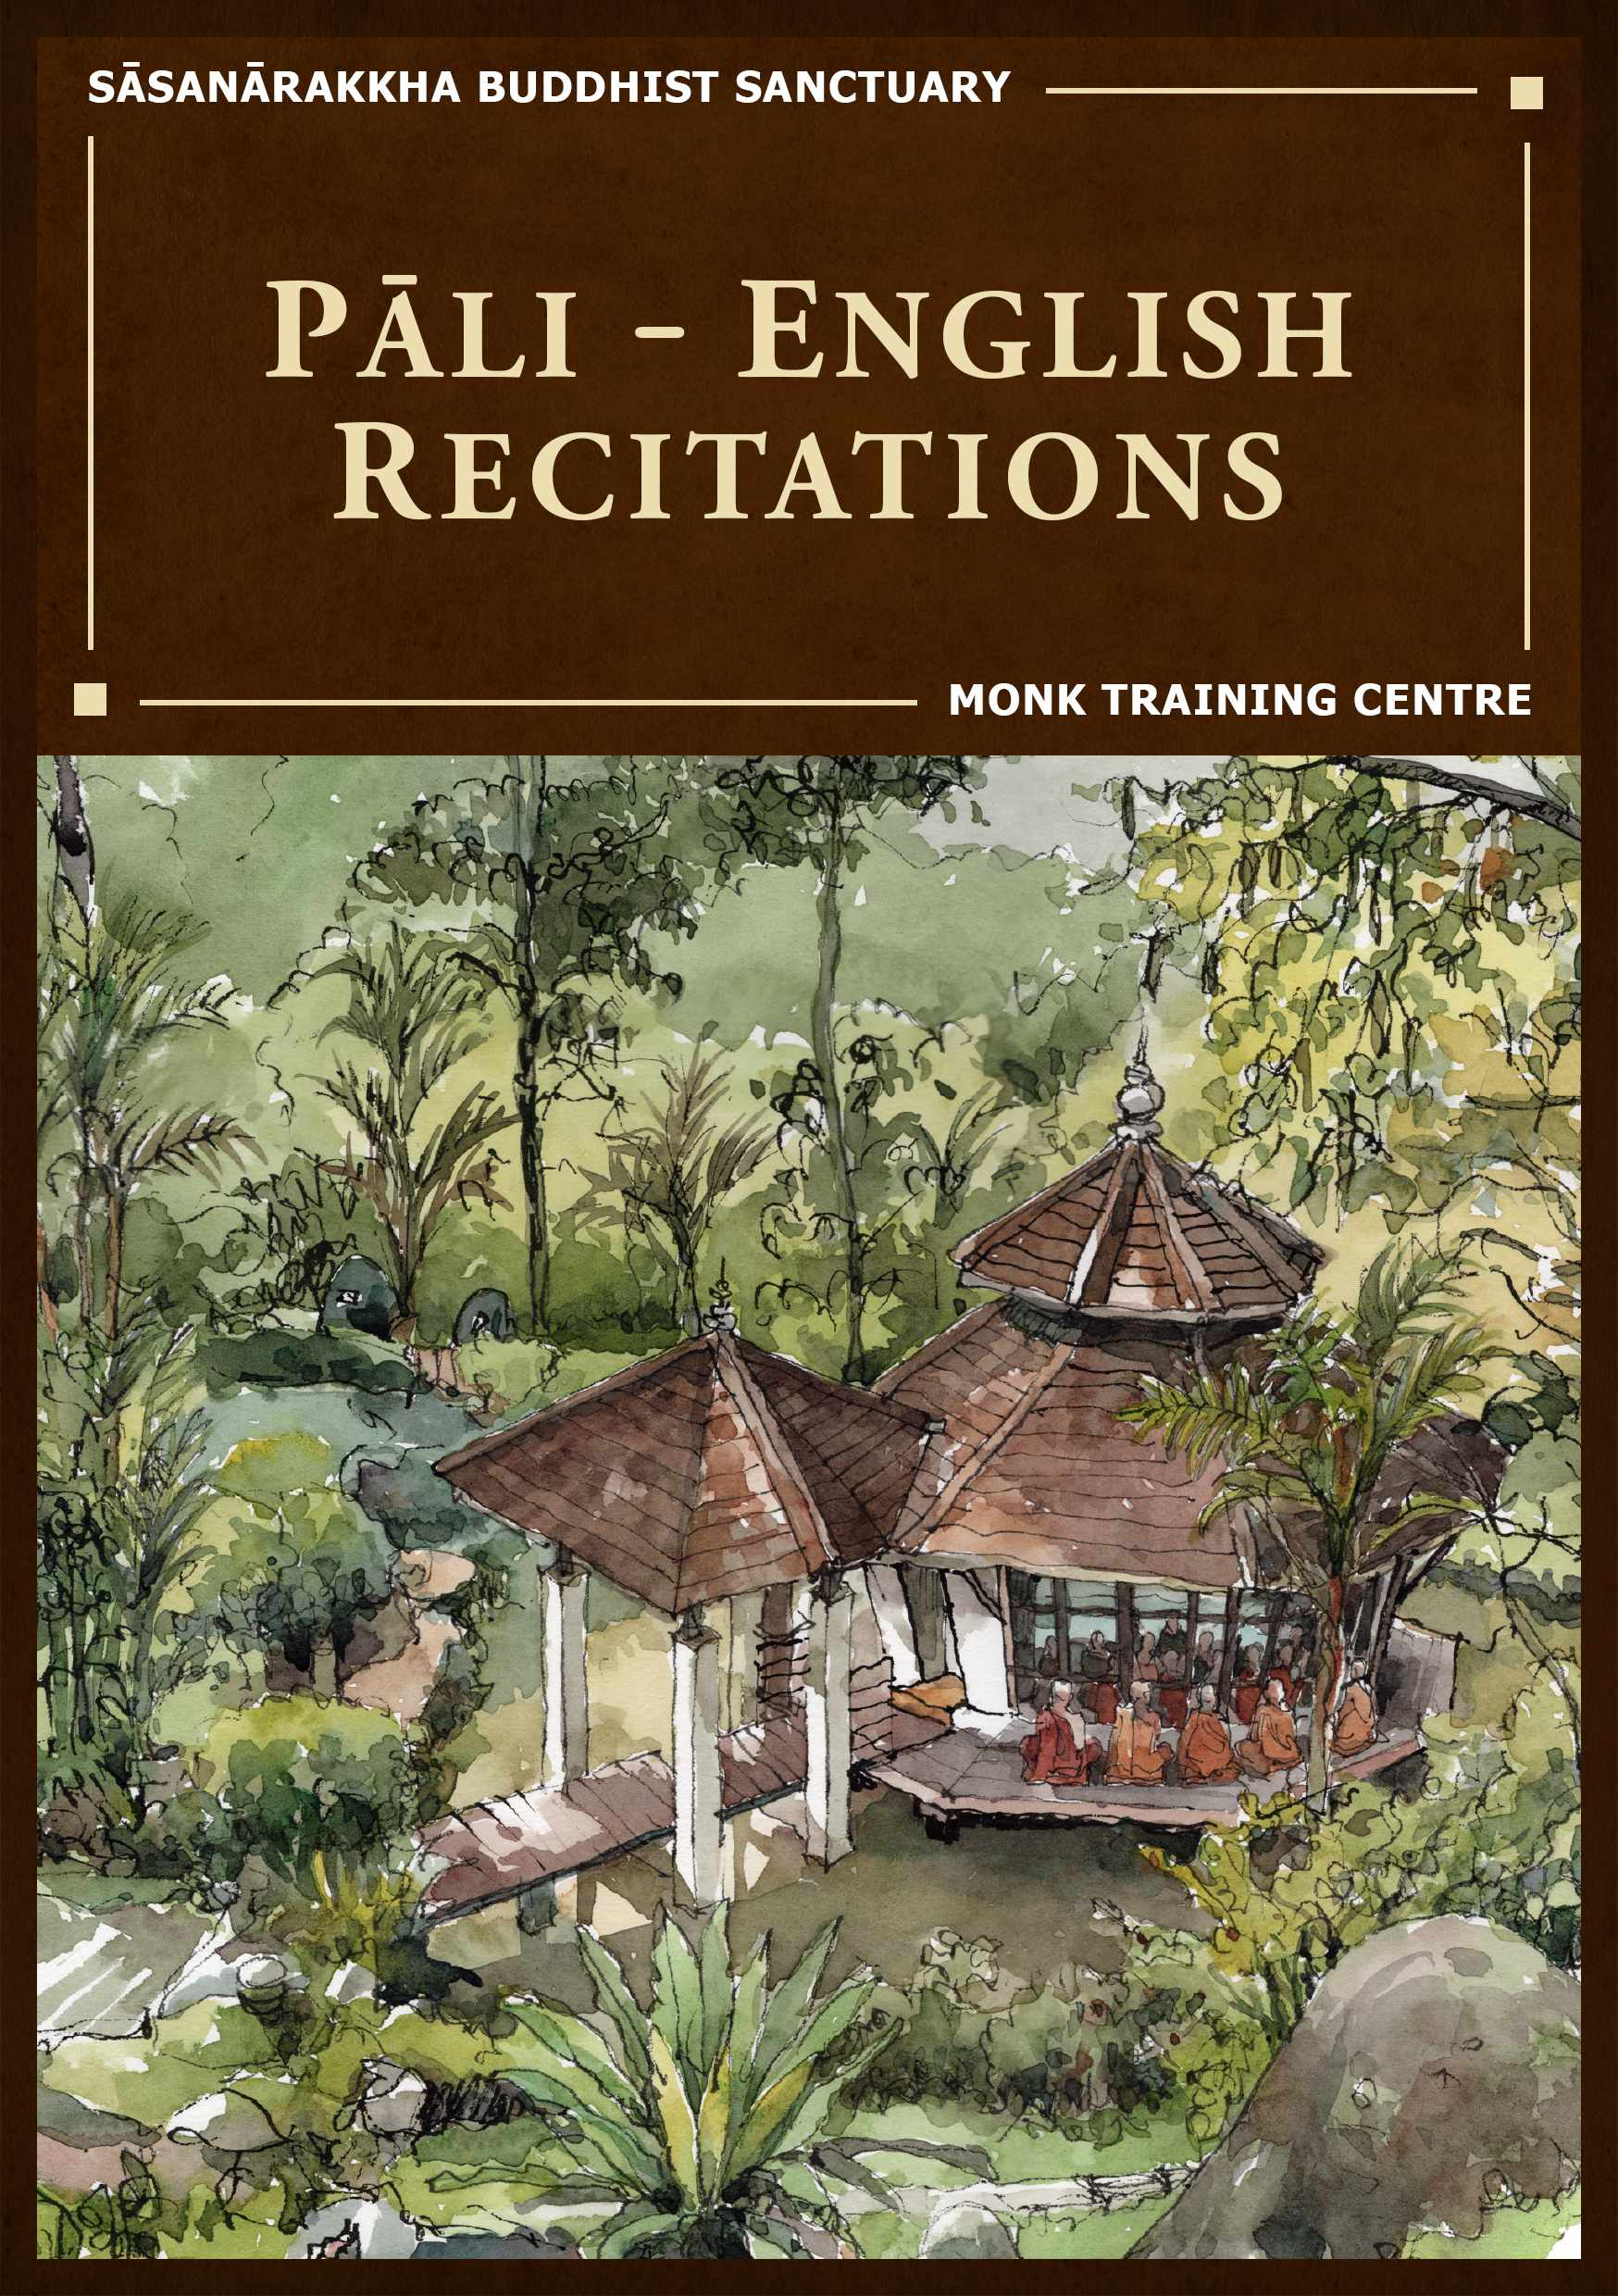
\includegraphics[height=\paperheight]{./front-cover-compressed.jpg}}
\fi

\pagestyle{empty}
\cleartorecto
\thispagestyle{empty}
\vspace*{3em}

{\centering

  \settowidth{\titleLength}{%
    {\Large\chapterTitleFont\textsc{\MakeUppercase{{\thetitle}}}}%
  }

  % 'SBS' on title page
  {\Huge\fontsize{64}{16}\sbsFont SBS}\\[1.0\baselineskip]%

  % 'Monk Training Centre'
  {\Huge\chapterTitleFont\textsc{{\thesubtitle\linebreak}}}\\[0.2\baselineskip]
  \setlength{\xheight}{\heightof{X}}

  % Ornament
  \raisebox{0.5\xheight}{\pgfornament[color=sbs-brown,width=7cm,scale=1,ydelta=0pt,symmetry=c]{84}}\\[1.4\baselineskip]

  % 'Pali-English Recitations'
  {\Large\scshape \thetitle}\\[2.5\baselineskip]

  % Dhamma quote
  {\quote ``The Blessed One who knows and sees, accomplished and fully enlightened, has prescribed the course of training for bhikkhus and he has laid down the Pātimokkha. On the Uposatha day as many of us as live in dependence upon a single village district meet together in unison, and when we meet we ask one who knows the Pātimokkha to recite it. If a bhikkhu remembers an offence or a transgression while the Pātimokkha is being recited, we make him act in accordance with the Dhamma, in accordance with the instructions. It is not the worthy ones that make us act; it is the Dhamma that makes us act.''\\ \smallskip (MN 108)}\\[1.4\baselineskip]
}

\cleartoverso
\thispagestyle{empty}

\vspace*{-\baselineskip}

{%

\fontsize{10}{16}\selectfont
\centering
\setlength{\parindent}{0pt}%
% \setlength{\parskip}{0.8\baselineskip}%

\vspace{0.5cm}

Published by TBD\\
% TODO need 2 ISBN numbers assigned (1 for print/pdf, 1 for epub); do more research before printing
% https://www.pnm.gov.my/
ISBN \theISBN\\
Copyright \copyright\ Sāsanārakkha Buddhist Sanctuary 2022

\vspace{0.5cm}

This book is for free distribution only;\\
it may not be sold.

\vspace{0.5cm}

Download this book as a PDF, EPUB, or MOBI\\
at the following address:\\
\href{https://sasanarakkha.org/}{https://sasanarakkha.org}

\vspace{0.5cm}

Project Manager: Ā. Ariyadhammika\\
Editor: Ā. Pāladhammika\\
Typesetting: Aj. Gambhiro, Ā. Pāladhammika\\
Translators: Ā. Ñāṇatusita\\
Endnotes: Ā. Ariyadhammika, Ā. Ṭhānissaro

\vspace{0.5cm}

This work is licensed under a Creative Commons\\
Attribution-NonCommercial-NoDerivatives 4.0 International~License.

Produced with the \LaTeX\ typesetting system,\\
set in Libertinus Serif.

\vspace{0.5cm}

\ifdesktopversion
This version was created on:\\
\today \space at \currenttime
\fi

\vspace{0.5cm}


\theEditionInfo

}

% \cleartorecto
\thispagestyle{empty}

{\setlength{\parskip}{10pt}

{\centering\fontsize{20}{25}\selectfont
\textsc{We Wish To Gratefully Acknowledge}
\par}

The Saṅghas of Wat Pah Nanachat (WPN), Amaravati, and Abhayagiri for allowing the use of material from their respective chanting books, the late Ven. Dr. Saddhātissa and Mr. Maurice Walshe for their English translations, as well as Ven. Bhikkhu Bodhi for granting permission to use and slightly adapt his translations. Further contributions are found on the previous page.

\vspace*{1.5\baselineskip}

Additional information on translations, as well as deviations\pagenote{%
  Due to the balanced and inspiring selction of chants, as well as for the sake of
  compatability, the WPN chanting book has served as the basis for the SBS
  chanting book. Over time, suggestions for the inclusion of additional chants, as
  well as occasional improvements of existing translations were incorporated. Such
  changes were meticulously marked down in the endnotes, so that someone familiar
  with the SBS chanting book can straight away find the relevant differences,
  which can be useful when visiting a branch monastery of the Ajahn Chah lineage,
  in order to know in which places to revert to the original version.}
from WPN Chanting Book (2014), have been annotated by Ven. Ariyadhammika in the endnotes.

\bigskip

{\centering
To Āyasmā Aggacitta, the founding father of\\
Sāsanārakkha Buddhist Sanctuary.

\bigskip

\includegraphics[height=65mm]{SBS_logo_Tuck_Loon_BAedit_2020_small.jpg}

}

}


\cleartorecto
\pagestyle{toponerow-frontmatter}
\chapterstyle{adrasteia-toc}

\pdfbookmark[section]{\contentsname}{toc}
\tableofcontents*

% \section{Abbreviations}

% \thispagestyle{empty}

% {\subsectionFmt{Abbreviations used in the text}}
% \bigskip

% {\raggedright
% \fontsize{10}{14}\selectfont

\begin{center}
  \begin{tabular}{@{}lll@{}}
    % [...  \hspace{-0.5mm}\anglebracketright\ & = & Only recited by the leader \\
    \breathmark\ & = & Take a breath \\
  \end{tabular}

  % Wisdom Publication sources: Nikāya and sutta # (eg. DN 1)
  % P.T.S. sources: Nikāya, volume #, page # (eg. D i 1)

  \begin{tabular}{@{}ll@{}}
    Vin   & Vinaya Piṭaka           \\
    DN    & Dīgha Nikāya            \\
    MN    & Majjhima Nikāya         \\
    SN    & Saṁyutta Nikāya         \\
    AN    & Aṅguttara Nikāya        \\
    Khp   & Khuddakapāṭha           \\
    Dhp   & Dhammapada              \\
    Ud    & Udāna                   \\
    Snp   & Sutta Nipāta            \\
    Thag  & Theragāthā              \\
    Ja    & Jātaka                  \\
    Ps    & Paṭisambhidāmagga       \\
    Vibh  & Abhidhamma Vibhaṅga     \\
    A     & Aṭṭhakathā              \\
    Dhs   & Dhammasaṅganī           \\
    A     & Aṭṭhakathā              \\
    A     & Aṭṭhakathā              \\
    MJG   & Mahā-jaya-maṅgala-gāthā \\
    Thai  & Composed...             \\
    Sri L & Composed...             \\
    Trad  & Tradtional...           \\
  \end{tabular}
\end{center}

% \bigskip

% Wisdom Publication sources: Nikāya and sutta # (eg. DN 1)
% P.T.S. sources: Nikāya, volume #, page # (eg. D i 1)

% References to shorter texts consisting of verses such as the Dhammapada, Udāna,
% Itivuttaka, Theragāthā, Therīgāthā or Sutta Nipāta are to the verse number or
% chapter and verse number. The other longer texts are referred to by volume and
% page number of the PTS edition.

% }


\chapterstyle{adrasteia-frontmatter}

\mainmatter
\pagestyle{toponerow}

\cleartorecto
% \part{Pāli}

{\raggedright
  \chapterOpeningPage{appendix-compressed.jpg}

\chapter{Pāli}

\clearpage

\section{Pubbakicca}
\label{pubbakicca}

\linkdest{endnote13-body}
\begin{intro}
  Okāsaṁ me bhante thero detu pāṭimokkhaṁ uddesituṁ.\makeatletter\hyperlink{endnote13-appendix}\Hy@raisedlink{\hypertarget{endnote13-body}{}{\pagenote{%
\hypertarget{endnote13-appendix}{\hyperlink{endnote13-body}{This is Dhammayuttika Nikāya version.}}}}}\makeatother\\
  \anglebracketleft\ \hspace{-0.5mm}Saṅghatthera: Karomi āyasmato okāsaṁ. \hspace{-0.5mm}\anglebracketright\
\end{intro}

\vspace{0.2cm}

Uposathakaraṇato pubbe navavidhaṁ pubbakiccaṁ kātabbaṁ hoti:

Taṇ'ṭhāna-sammajjanañ'ca; tattha padīp'ujjalanañ'ca; āsana-paññapanañ'ca; pānīyaparibhojanīy'ūpaṭṭhapanañ'ca; chand'ārahānaṁ bhikkhūnaṁ chand'āharaṇañ'ca; tesaññ'eva akat'uposathānaṁ pārisuddhiyā'pi āharaṇañ'ca; utu'kkhānañ'ca; bhikkhugaṇanā ca; bhikkhunīnam'ovādo cā'ti.

\linkdest{endnote1-body}
Tattha purimesu catūsu kiccesu padīpakiccaṁ idāni suriy'ālokassa atthitāya n'atthi, aparāni tīṇi\makeatletter\hyperlink{endnote1-appendix}\Hy@raisedlink{\hypertarget{endnote1-body}{}{\pagenote{%
      \hypertarget{endnote1-appendix}{\hyperlink{endnote1-body}{\textit{If the recitation is held at night, change:}\\
          \smallskip
          ``Tattha purimesu catūsu kiccesu padīpa-kiccaṁ idāni suriy'ālokassa atthitāya n'atthi.
          Aparāni tīṇi'' to ``Tattha purimāni cattāri'' (``\textit{Of the first four…}'')}}}}}\makeatother
\linkdest{endnote2-body}
bhikkhūnaṁ vattaṁ jānantehi bhikkhūhi\makeatletter\hyperlink{endnote2-appendix}\Hy@raisedlink{\hypertarget{endnote2-body}{}{\pagenote{%
      \hypertarget{endnote2-appendix}{\hyperlink{endnote2-body}{\textit{If sāmaṇeras help with the tasks, change to:}\\
          \smallskip
          ``bhikkhūhi'' to ``sāmaṇerehi'pi bhikkhūhi'pi'' (``\textit{Novices and bhikkhus…}'')\\
          \smallskip
          \textit{If laypeople living in the monastery help with the tasks, change to:}\\
          \smallskip
          ``ārāmikehi'pi bhikkhūhi'pi'' (``\textit{Monastery dwellers and bhikkhus…}'')}}}}}\makeatother
\linkdest{endnote2-body}
katāni pariniṭṭhitāni honti.\makeatletter\hyperlink{endnote3-appendix}\Hy@raisedlink{\hypertarget{endnote3-body}{}{\pagenote{%
      \hypertarget{endnote3-appendix}{\hyperlink{endnote3-body}{If there are bhikkhus outside of hatthapāsa but within the sīmā (territory) who have sent their consent and purity, then for a recitation during the day, the entire passage within brackets should be:
          \smallskip
          ``Tattha purimesu chasu kiccesu padīpa-kiccaṁ idāni suriy'ālokassa atthitāya n'atthi. Aparāni pañca bhikkhūnaṁ vattaṁ jānantehi bhikkhūhi katāni pariniṭṭhitāni honti.''
          \smallskip
          For a recitation at night in the same situation, the entire passage should be:
          \smallskip
          ``Tattha purimāni cha bhikkhūnaṁ vattaṁ jānantehi katāni pariniṭṭhitāni honti''.}}}}}\makeatother

Chand'āharaṇa pārisuddhi-āharaṇāni pana imissaṁ sīmāyaṁ hatthapāsaṁ vijahitvā nisinnānaṁ bhikkhūnaṁ abhāvato n'atthi. Utu'kkhānaṁ nāma ettakaṁ atikkantaṁ ettakaṁ avasiṭṭhan'ti; evaṁ utu-ācikkhanaṁ. Utūn'īdha pana sāsane hemanta-gimha-vassānānaṁ vasena tīṇi honti.

\linkdest{endnote4-body}
Ayaṁ hemanto'tu\makeatletter\hyperlink{endnote4-appendix}\Hy@raisedlink{\hypertarget{endnote4-body}{}{\pagenote{%
      \hypertarget{endnote4-appendix}{\hyperlink{endnote4-body}{During the hot season, change: ``hemanto'tu'' to ``gimho'tu'' and during the rainy season: ``vassāno'tu''.}}}}}\makeatother
\linkdest{endnote5-body}
asmiñ'ca utumhi aṭṭha uposathā,\makeatletter\hyperlink{endnote5-appendix}\Hy@raisedlink{\hypertarget{endnote5-body}{}{\pagenote{%
      \hypertarget{endnote5-appendix}{\hyperlink{endnote5-body}{During a normal rainy season, change to:\\
          ``aṭṭha uposathā'' to ``sattā ca uposathā ekā ca pavāraṇā'' (``Seven uposathas and one pavāraṇā.'')\\
          \smallskip
          During a hot or cold season with an additional month, change to:\\
          ``adhikamāsa-vasena dasa uposathā'' (``Because of the additional month, ten uposathās…''.)\\
          \smallskip
          During a rainy season with an additional month, change to:\\
          ``adhikamāsa-vasena nava ca uposathā ekā ca pavāraṇā'' (``Because of the additional month, nine uposathas and one pavāraṇā…''.)}}}}}\makeatother
\linkdest{endnote6-body}
iminā pakkhena: eko uposatho sampatto, dve uposathā atikkantā, pañca uposathā avasiṭṭhā.\makeatletter\hyperlink{endnote6-appendix}\Hy@raisedlink{\hypertarget{endnote6-body}{}{\pagenote{%
      \hypertarget{endnote6-appendix}{\hyperlink{endnote6-body}{This is the calculation for the first uposatha in a normal hot or cold season. The calculation for other dates — to be stated after ``iminā pakkhena eko uposatho sampatto'' — is as follows:\smallskip \\
          During a normal hot or cold season:\\
          Second: eko uposatho atikkanto, cha uposathā avasiṭṭhā.\\
          Third: dve uposathā atikkantā, pañca uposathā avasiṭṭhā.\\
          Fourth: tayo uposathā atikkantā, cattāro uposathā avasiṭṭhā.\\
          Fifth: cattāro uposathā atikkantā, tayo uposathā avasiṭṭhā.\\
          Sixth: pañca uposathā atikkantā, dve uposathā avasiṭṭhā.\\
          Seventh: cha uposathā atikkantā, eko uposatho avasiṭṭho.\\
          \smallskip
          Eighth: satta uposathā atikkantā, aṭṭha uposathā paripuṇṇā.\\
          During a normal rainy season:\\
          First: cha ca uposathā ekā ca pavāraṇā avasiṭṭhā.\\
          Second: eko uposatho atikkanto, pañca ca uposathā ekā ca pavāraṇā avasiṭṭhā.\\
          Third: dve uposathā atikkantā, cattāro ca uposathā ekā ca pavāraṇā avasiṭṭhā.\\
          Fourth: tayo uposathā atikkantā, tayo ca uposathā ekā ca pavāraṇā avasiṭṭhā.\\
          Fifth: cattāro uposathā atikkantā, dve ca uposathā ekā ca pavāraṇā avasiṭṭhā.\\
          Sixth: (see the separate section on the Pavāraṇā.)\\
          Seventh: pañca ca uposathā ekā ca pavāraṇā atikkantā, eko uposatho avasiṭṭho.\\
          Eighth: cha ca uposathā ekā ca pavāraṇā atikkantā, satta ca uposathā ekā ca pavāraṇā paripuṇṇā.\smallskip \\
          During a hot or cold season with an additional month:\\
          First: nava uposathā avasiṭṭhā.\\
          Second: eko uposatho atikkanto, aṭṭha uposathā avasiṭṭhā.\\
          Third: dve uposathā atikkantā, satta uposathā avasiṭṭhā.\\
          Fourth: tayo uposathā atikkantā, cha uposathā avasiṭṭhā.\\
          Fifth: cattāro uposathā atikkantā, pañca uposathā avasiṭṭhā.\\
          Sixth: pañca uposathā atikkantā, cattāro uposathā avasiṭṭhā.\\
          Seventh: cha uposathā atikkantā, tayo uposathā avasiṭṭhā.\\
          Eighth: satta uposathā atikkantā, dve uposathā avasiṭṭhā.\\
          Ninth: aṭṭha uposathā atikkantā, eko uposatho avasiṭṭho.\\
          \smallskip
          Tenth: nava uposathā atikkantā, dasa uposathā paripuṇṇā.\\
          During a rainy season with an additional month:\\
          First: aṭṭha ca uposathā ekā ca pavāraṇā avasiṭṭhā.\\
          Second: eko uposatho atikkanto, satta ca uposathā ekā ca pavāraṇā avasiṭṭhā.\\
          Third: dve uposathā atikkantā, cha ca uposathā ekā ca pavāraṇā avasiṭṭhā.\\
          Fourth: tayo uposathā atikkantā, pañca ca uposathā ekā ca pavāraṇā avasiṭṭhā.\\
          Fifth: cattāro uposathā atikkantā, cattāro ca uposathā ekā ca pavāraṇā avasiṭṭhā.\\
          Sixth: pañca uposathā atikkantā, tayo ca uposathā ekā ca pavāraṇā avasiṭṭhā.\\
          Seventh: cha uposathā atikkantā, dve ca uposathā ekā ca pavāraṇā avasiṭṭhā.\\
          Eighth: (see the separate section on the Pavāraṇā.)\\
          Ninth: satta ca uposathā ekā ca pavāraṇā atikkantā, eko uposatho avasiṭṭho.\\
          Tenth: aṭṭha ca uposathā ekā ca pavāraṇā atikkantā, nava ca uposathā ekā ca pavāraṇā paripuṇṇā.}}}}}\makeatother \thickspace
Iti evaṁ sabbehi āyasmantehi utu'kkhānaṁ dhāretabbaṁ.

\begin{center}
  \anglebracketleft\ \hspace{-0.5mm}Everyone: ``Evaṁ bhante / āvuso'' \hspace{-0.5mm}\anglebracketright\
\end{center}

\linkdest{endnote7-body}
Bhikkhugaṇanā nāma imasmiṁ uposath'agge uposath'atthāya sannipatitā bhikkhū ettakā'ti, bhikkhūnaṁ gaṇanā. Imasmiṁ pana uposath'agge cattāro\makeatletter\hyperlink{endnote7-appendix}\Hy@raisedlink{\hypertarget{endnote7-body}{}{\pagenote{%
      \hypertarget{endnote7-appendix}{\hyperlink{endnote7-body}{Cattāro = four. This should be replaced with the actual number of bhikkhus present. 5 pañca 6 cha 7 satta 8 aṭṭha 9 nava 10 dasa 11 ekādasa 12 dvādasa, bārasa 13 terasa, teḷasa 14 catuddasa, cuddasa
          15 paṇṇarasa, pañcadasa 16 soḷasa 17 sattarasa 18 aṭṭhārasa, aṭṭhādasa 19 ekūnavīsati 20 vīsati, vīsa 21 ekavīsati 22 dvāvīsati, dvāvīsa, dvevīsati, bāvīsati, bāvīsa 23 tevīsati 24 catuvīsati 25 pañcavīsati 26 chabbīsati 27 sattavīsati 28 aṭṭhavīsati 29 ekūnatiṁsa 30 tiṁsa, samatiṁsa, tiṁsati 31 ekatiṁsa, ekattiṁsa 32 dvattiṁsa 33 tettiṁsa 34 catuttiṁsa 35 pañcattiṁsa 36 chattiṁsa 37 sattattiṁsa 38 aṭṭhattiṁsa 39 ekūnacattāḷīsa40 cattāḷīsa, cattārīsa 41 ekacattāḷīsa 42 dvacattāḷīsa, dvecattāḷīsa, dvicattāḷīsa 43 tecattāḷīsa 44 catucattāḷīsa 45 pañcacattāḷīsa 46 chacattāḷīsa 47 sattacattāḷīsa 48 aṭṭhacattāḷīsa 49 ekūnapaññāsa 50 paññāsa 51 ekapaññāsa 52 dvapaññāsa, dvepaññāsa, dvipaññāsa 53 tepaññāsa 54 catupaññāsa 55 pañcapaññāsa 56 chapaññāsa 57 sattapaññāsa 58 aṭṭhapaññāsa 59 ekūnasaṭṭhī 60 saṭṭhī, saṭṭhi 61 ekasaṭṭhī 62 dvāsaṭṭhī, dvesaṭṭhī, dvisaṭṭhī 63 tesaṭṭhī 64 catusaṭṭhī 65 pañcasaṭṭhī 66 chasaṭṭhī 67 sattasaṭṭhī 68 aṭṭhasaṭṭhī 69 ekūnasattati 70 sattati 71 ekasattati 72 dvasattati, dvāsattati, dvesattati, dvisattati 73 tesattati 74 catusattati 75 pañcasattati 76 chasattati 77 sattasattati 78 aṭṭhasattati 79 ekūnāsīti 80 asīti 81 ekāsīti 82 dvāsīti 83 tayāsīti 84 caturāsīti 85 pañcāsīti 86 chaḷāsīti 87 sattāsīti 88 aṭṭhāsīti 89 ekūnanavuti 90 navuti 91 ekanavuti 92 dvanavuti, dvenavuti 93 tenavuti 94 catunavuti 95 pañcanavuti 96 chanavuti 97 sattanavuti 98 aṭṭhanavuti 99 ekūnasataṁ 100 bhikkhusataṁ 101 ekuttara-bhikkhusataṁ 102 dvayuttara-bhikkhusataṁ 103 tayuttara-bhikkhusataṁ 104 catuttara-bhikkhusataṁ 105 pañcuttara-bhikkhusataṁ 106 chaḷuttara-bhikkhusataṁ 107 sattuttara-bhikkhusataṁ 108 aṭṭhuttara-bhikkhusataṁ 109 navuttara-bhikkhusataṁ 110 dasuttara-bhikkhusataṁ 120 vīsuttara-bhikkhusataṁ 130 tiṁsuttara-bhikkhusataṁ 140 cattāḷīsuttara-bhikkhusataṁ 150 paññāsuttara-bhikkhusataṁ 160 saṭṭhayuttara-bhikkhusataṁ 170 sattatyuttara-bhikkhusataṁ 180 asītyuttara-bhikkhusataṁ 190 navutyuttara-bhikkhusataṁ 199 ekūnasatuttara-bhikkhusataṁ 200 dve bhikkhu-satāni 201 ekuttarāni dve bhikkhu-satāni 300 tayo bhikkhu-satāni 400 cattāro bhikkhu-satāni 500 pañca bhikkhu-satāni
          \smallskip
          All numbers ending with ``bhikkhusataṁ'' should be followed by ``sannipatitaṁ hoti''.
          \smallskip
          All numbers ending with ``bhikkhusatāni'' should be followed by ``sannipatitā honti''.}}}}}\makeatother \thickspace
bhikkhū sannipatitā honti. Iti sabbehi āyasmantehi bhikkhugaṇanā'pi dhāretabbā.

\begin{center}
  \anglebracketleft\ \hspace{-0.5mm}Everyone: ``Evaṁ bhante / āvuso'' \hspace{-0.5mm}\anglebracketright\
\end{center}

Bhikkhunīnam'ovādo pana samīpe tāsaṁ n'atthitāya n'atthi.

Iti sakaraṇ'okāsānaṁ pubbakiccānaṁ katattā nikkaraṇ'okāsānaṁ pubbakiccānaṁ pakatiyā pariniṭṭhitattā evan'taṁ navavidhaṁ pubbakiccaṁ pariniṭṭhitaṁ hoti.

Niṭṭhite ca pubbakicce: Sace so divaso cātuddasī-paṇṇarasī-sāmaggīnam'aññataro yath'ājja uposatho paṇṇaraso / cātuddaso / sāmaggo.

\begin{enumerate}
  \item Yāvatikā ca bhikkhū kammappattā saṅghuposath'ārahā cattāro vā tato vā atirekā pakatattā pārājikaṁ anāpannā saṅghena vā anukkhittā.
  \item Te ca kho hatthapāsaṁ avijahitvā ekasīmāyaṁ ṭhitā.
  \item Tesañ'ca vikālabhojan'ādi-vasena-vatthu-sabhāg'āpattiyo ce na vijjanti.
  \item Tesañ'ca hatthapāse hatthapāsato bahikaraṇavasena vajjetabbo koci vajjanīyapuggalo ce n'atthi.
\end{enumerate}

Evan'taṁ uposathakammaṁ imehi catūhi lakkhaṇehi saṅgahitaṁ pattakallaṁ nāma hoti, kātuṁ yuttarūpaṁ.

Uposathakammassa pattakallattaṁ viditvā idāni kariyamāno uposatho saṅghena anumānetabbo.


\begin{center}
  \anglebracketleft\ \hspace{-0.5mm}Everyone: ``Sādhu bhante / āvuso'' \hspace{-0.5mm}\anglebracketright\
\end{center}

\begin{center}
  \anglebracketleft\ \hspace{-0.5mm}Saṅghatthera: Pubbakaraṇa-pubbakiccāni samāpetvā, imassa nisinnassa bhikkhusaṅghassa anumatiyā pāṭimokkhaṁ uddesituṁ ajjhesanaṁ karomi. \hspace{-0.5mm}\anglebracketright\
\end{center}

\clearpage

  \section{Nidān'uddeso}
\label{nidan'uddeso}

Suṇātu me bhante / āvuso saṅgho, ajj'uposatho paṇṇaraso / cātuddaso / sāmaggo, yadi saṅghassa pattakallaṁ, saṅgho uposathaṁ kareyya pātimokkhaṁ uddiseyya.

Kiṁ saṅghassa pubbakiccaṁ?

Pārisuddhiṁ āyasmanto ārocetha. Pātimokkhaṁ uddisissāmi. Taṁ sabb'eva santā sādhukaṁ suṇoma manasikaroma. Yassa siyā āpatti, so āvikareyya. Asantiyā āpattiyā, tuṇhī bhavitabbaṁ. Tuṇhībhāvena kho pan'āyasmante parisuddhā'ti vedissāmi.

Yathā kho pana paccekapuṭṭhassa veyyākaraṇaṁ hoti, evam'evaṁ evarūpāya parisāya yāvatatiyaṁ anussāvitaṁ hoti. Yo pana bhikkhu yāvatatiyaṁ anussāviyamāne saramāno santiṁ āpattiṁ nāvikareyya, sampajānamusāvād'assa hoti. Sampajānamusāvādo kho pan'āyasmanto antarāyiko dhammo vutto bhagavatā. Tasmā saramānena bhikkhunā āpannena visuddh'āpekkhena santī āpatti āvikātabbā, āvikatā hi'ssa phāsu hoti.

\medskip

\linkdest{endnote8-body}
\begin{center}
Uddiṭṭhaṃ kho āyasmanto nidānaṃ.\makeatletter\hyperlink{endnote8-appendix}\Hy@raisedlink{\hypertarget{endnote8-body}{}{\pagenote{%
  \hypertarget{endnote8-appendix}{\hyperlink{endnote8-body}{This can be skipped since it doesn't occur in the Canon. The Nidāna can instead be concluded with ``Nidānaṁ niṭṭhitaṁ.''}}}}}\makeatother

\smallskip

Tatth'āyasmante pucchāmi: Kacci'ttha parisuddhā?\\
Dutiyam'pi pucchāmi: Kacci'ttha parisuddhā?\\
Tatiyam'pi pucchāmi: Kacci'ttha parisuddhā?

\smallskip

Parisuddh'etth'āyasmanto, tasmā tuṇhī, evam'etaṁ dhārayāmi.
\end{center}

\linkdest{endnote9-body}
\begin{outro}
  Nidānaṃ niṭṭhitaṃ\makeatletter\hyperlink{endnote9-appendix}\Hy@raisedlink{\hypertarget{endnote9-body}{}{\pagenote{%
    \hypertarget{endnote9-appendix}{\hyperlink{endnote9-body}{Not in any edition or manuscript, but if a conclusion is to be recited then this one as given in the Parivāra would be the suitable one.\\
	When reciting in brief use: Nidān'uddeso niṭṭhito.}}}}}\makeatother
\end{outro}

\clearpage

  \section{Pārājik'uddeso}
\label{par}

\begin{intro}
  Tatr'ime cattāro pārājikā dhammā uddesaṁ āgacchanti.
\end{intro}

\setsubsecheadstyle{\subsubsectionFmt}
\pdfbookmark[2]{Pārājika 1}{par1}
\subsection*{\hyperref[disq1]{Pārājika 1: Methunadhammasikkhāpadaṁ}}
\label{par1}

Yo pana bhikkhu bhikkhūnaṁ sikkhā-sājīva-samāpanno, sikkhaṁ appaccakkhāya dubbalyaṁ anāvikatvā, methunaṁ dhammaṁ paṭiseveyya antamaso tiracchāna-gatāya-pi: pārājiko hoti asaṁvāso.

\pdfbookmark[2]{Pārājika 2}{par2}
\subsection*{\hyperref[disq2]{Pārājika 2: Adinn'ādānasikkhāpadaṁ}}
\label{par2}

Yo pana bhikkhu sañcicca manussa-viggahaṁ jīvitā voropeyya, satthahārakaṁ vā'ssa pariyeseyya, maraṇa-vaṇṇaṁ vā saṁvaṇṇeyya, maraṇāya vā samādapeyya, “Ambho purisa kiṁ tuyh’iminā pāpakena dujjīvitena? Matan-te jīvitā seyyo” ti. Iti cittamano citta-saṅkappo aneka-pariyāyena maraṇa-vaṇṇaṁ vā saṁvaṇṇeyya, maraṇāya vā samādapeyya: ayam'pi pārājiko hoti asaṁvāso.

\pdfbookmark[2]{Pārājika 3}{par3}
\subsection*{\hyperref[disq3]{Pārājika 3: Manussaviggahasikkhāpadaṁ}}
\label{par3}

Yo pana bhikkhu anabhijānaṁ uttari-manussa-dhammaṁ attūpanāyikaṁ alam-ariya-ñāṇa-dassanaṁ samudācareyya: “Iti jānāmi, iti passāmī” ti. Tato aparena samayena samanuggāhiyamāno vā asamanuggāhiyamāno vā āpanno visuddh’āpekkho evaṁ vadeyya, “Ajānam-evaṁ āvuso avacaṁ, ‘jānāmi,’ apassaṁ, ‘passāmi.’ Tucchaṁ musā vilapin” ti. Aññatra adhimānā: ayam'pi pārājiko hoti asaṁvāso.

\pdfbookmark[2]{Pārājika 4}{par4}
\subsection*{\hyperref[disq4]{Pārājika 4: Uttarimanussadhammasikkhāpadaṁ}}
\label{par4}

Yo pana bhikkhu anabhijānaṁ uttari-manussa-dhammaṁ attūpanāyikaṁ alam-ariya-ñāṇa-dassanaṁ samudācareyya: “Iti jānāmi, iti passāmī” ti. Tato aparena samayena samanuggāhiyamāno vā asamanuggāhiyamāno vā āpanno visuddh’āpekkho evaṁ vadeyya, “Ajānam-evaṁ āvuso avacaṁ, ‘jānāmi,’ apassaṁ, ‘passāmi.’ Tucchaṁ musā vilapin” ti. Aññatra adhimānā: ayam'pi pārājiko hoti asaṁvāso.

\medskip

\begin{center}
Uddiṭṭhā kho āyasmanto cattāro pārājikā dhammā, yesaṁ bhikkhu aññataraṁ vā aññataraṁ vā āpajjitvā na labhati bhikkhūhi saddhiṁ saṁvāsaṁ. Yathā pure, tathā pacchā: pārājiko hoti asaṁvāso.

\smallskip

Tatth'āyasmante pucchāmi: Kacci'ttha parisuddhā?\\
Dutiyam'pi pucchāmi: Kacci'ttha parisuddhā?\\
Tatiyam'pi pucchāmi: Kacci'ttha parisuddhā?

\smallskip

Parisuddh'etth'āyasmanto, tasmā tuṇhī, evam'etaṁ dhārayāmi.
\end{center}

\begin{outro}
  Pārājik’uddeso niṭṭhito
\end{outro}

\clearpage

  \setsecheadstyle{\sectionFmt}
\section{Saṅghādises'uddeso}
\label{sd}

\begin{intro}
  Ime kho pan'āyasmanto terasa saṅghādisesā dhammā uddesaṁ āgacchanti.
\end{intro}

\pdfbookmark[2]{Saṅghādisesa 1}{sd1}
\subsection*{\hyperref[comm1]{Saṅghādisesa 1: Sukkavissaṭṭhisikkhāpadaṁ}}
\label{sd1}
Sañcetanikā sukka-visaṭṭhi aññatra supinantā, saṅghādiseso.

\pdfbookmark[2]{Saṅghādisesa 2}{sd2}
\subsection*{\hyperref[comm2]{Saṅghādisesa 2: Kāyasaṁsaggasikkhāpadaṁ}}
\label{sd2}
Yo pana bhikkhu otiṇṇo vipariṇatena cittena mātugāmena saddhiṁ kāya-saṁsaggaṁ samāpajjeyya, hattha-gāhaṁ vā veṇi-gāhaṁ vā aññatarassa vā aññatarassa vā aṅgassa parāmasanaṁ, saṅghādiseso.

\pdfbookmark[2]{Saṅghādisesa 3}{sd3}
\subsection*{\hyperref[comm3]{Saṅghādisesa 3: Duṭṭhullavācāsikkhāpadaṁ}}
\label{sd3}
Yo pana bhikkhu otiṇṇo vipariṇatena cittena mātugāmaṁ duṭṭhullāhi vācāhi obhāseyya, yathā taṁ yuvā yuvatiṁ methunūpasañhitāhi, saṅghādiseso.

\pdfbookmark[2]{Saṅghādisesa 4}{sd4}
\subsection*{\hyperref[comm4]{Saṅghādisesa 4: Attakāmapāricariyasikkhāpadaṁ}}
\label{sd4}
Yo pana bhikkhu otiṇṇo vipariṇatena cittena mātugāmassa santike atta-kāma-pāricariyāya vaṇṇaṁ bhāseyya, “Etad-aggaṁ bhagini pāricariyānaṁ, yā m’ādisaṁ sīlavantaṁ kalyāṇa-dhammaṁ brahmacāriṁ etena dhammena paricareyyā” ti, methunūpasañhitena, saṅghādiseso.

\pdfbookmark[2]{Saṅghādisesa 5}{sd5}
\subsection*{\hyperref[comm5]{Saṅghādisesa 5: Sañcarittasikkhāpadaṁ}}
\label{sd5}
Yo pana bhikkhu sañcarittaṁ samāpajjeyya, itthiyā vā purisa-matiṁ, purisassa vā itthī-matiṁ, jāyattane vā jārattane vā antamaso taṁ-khaṇikāya-pi, saṅghādiseso.

\pdfbookmark[2]{Saṅghādisesa 6}{sd6}
\subsection*{\hyperref[comm6]{Saṅghādisesa 6: Kuṭikārasikkhāpadaṁ}}
\label{sd6}
Saññācikāya pana bhikkhunā kuṭiṁ kārayamānena assāmikaṁ att’uddesaṁ pamāṇikā kāretabbā. Tatr’idaṁ pamāṇaṁ: dīghaso dvādasa vidatthiyo sugata-vidatthiyā, tiriyaṁ satt’antarā. Bhikkhū abhinetabbā vatthu-desanāya. Tehi bhikkhūhi vatthuṁ desetabbaṁ anārambhaṁ saparikkamanaṁ. Sārambhe ce bhikkhu vatthusmiṁ aparikkamane saññācikāya kuṭiṁ kāreyya, bhikkhū vā anabhineyya vatthu-desanāya, pamāṇaṁ vā atikkāmeyya, saṅghādiseso.

\pdfbookmark[2]{Saṅghādisesa 7}{sd7}
\subsection*{\hyperref[comm7]{Saṅghādisesa 7: Vihārakārasikkhāpadaṁ}}
\label{sd7}
Mahallakam-pana bhikkhunā vihāraṁ kārayamānena, sassāmikaṁ att’uddesaṁ bhikkhū abhinetabbā vatthu-desanāya. Tehi bhikkhūhi vatthuṁ desetabbaṁ anārambhaṁ saparikkamanaṁ. Sārambhe ce bhikkhu vatthusmiṁ aparikkamane mahallakaṁ vihāraṁ kāreyya, bhikkhū vā anabhineyya vatthu-desanāya, saṅghādiseso.

\pdfbookmark[2]{Saṅghādisesa 8}{sd8}
\subsection*{\hyperref[comm8]{Saṅghādisesa 8: Duṭṭhadosasikkhāpadaṁ}}
\label{sd8}
Yo pana bhikkhu bhikkhuṁ duṭṭho doso appatīto amūlakena pārājikena dhammena anuddhaṁseyya, “App’eva nāma naṁ imamhā brahmacariyā cāveyyan” ti. Tato aparena samayena samanuggāhiyamāno vā asamanuggāhiyamāno vā, amūlakañ-c’eva taṁ adhikaraṇaṁ hoti, bhikkhu ca dosaṁ patiṭṭhāti, saṅghādiseso.

\pdfbookmark[2]{Saṅghādisesa 9}{sd9}
\subsection*{\hyperref[comm9]{Saṅghādisesa 9: Aññabhāgiyasikkhāpadaṁ}}
\label{sd9}
Yo pana bhikkhu bhikkhuṁ duṭṭho doso appatīto aññabhāgiyassa adhikaraṇassa kiñci desaṁ lesa-mattaṁ upādāya pārājikena dhammena anuddhaṁseyya, “App’eva nāma naṁ imamhā brahmacariyā cāveyyan” ti. Tato aparena samayena samanuggāhiyamāno vā asamanuggāhiyamāno vā, aññabhāgiyañ-c’eva taṁ adhikaraṇaṁ hoti, koci deso lesa-matto upādinno, bhikkhu ca dosaṁ patiṭṭhāti, saṅghādiseso.

\pdfbookmark[2]{Saṅghādisesa 10}{sd10}
\subsection*{\hyperref[comm10]{Saṅghādisesa 10: Saṅghabhedasikkhāpadaṁ}}
\label{sd10}
Yo pana bhikkhu samaggassa saṅghassa bhedāya parakkameyya, bhedana-saṁvattanikaṁ vā adhikaraṇaṁ samādāya paggayha tiṭṭheyya, so bhikkhu bhikkhūhi evam-assa vacanīyo, “Mā āyasmā samaggassa saṅghassa bhedāya parakkami. Bhedana-saṁvattanikaṁ vā adhikaraṇaṁ samādāya paggayha aṭṭhāsi. Samet’āyasmā saṅghena, samaggo hi saṅgho sammodamāno avivadamāno ek’uddeso phāsu viharatī” ti. Evañ-ca so bhikkhu bhikkhūhi vuccamāno tath’eva paggaṇheyya, so bhikkhu bhikkhūhi yāva-tatiyaṁ samanubhāsitabbo tassa paṭinissaggāya. Yāva-tatiyañ-ce samanubhāsiyamāno taṁ paṭinissajjeyya, icc’etaṁ kusalaṁ. No ce paṭinissajjeyya, saṅghādiseso.

\pdfbookmark[2]{Saṅghādisesa 11}{sd11}
\subsection*{\hyperref[comm11]{Saṅghādisesa 11: Bhed'ānuvattakasikkhāpadaṁ}}
\label{sd11}
Tass’eva kho pana bhikkhussa bhikkhū honti anuvattakā vagga-vādakā, eko vā dve vā tayo vā, te evaṁ vadeyyuṁ, “Mā āyasmanto etaṁ bhikkhuṁ kiñci avacuttha. Dhamma-vādī c’eso bhikkhu, vinaya-vādī c’eso bhikkhu, amhākañ-c’eso bhikkhu chandañ-ca ruciñ-ca ādāya voharati. Jānāti no bhāsati, amhākam-p’etaṁ khamatī” ti. Te bhikkhū bhikkhūhi evam-assu vacanīyā, “Mā āyasmanto evaṁ avacuttha. Na c’eso bhikkhu dhamma-vādī, na c’eso bhikkhu vinaya-vādī. Mā āyasmantānam'pi saṅgha-bhedo rucittha. Samet‘'āyasmantānaṁ saṅghena, samaggo hi saṅgho sammodamāno avivadamāno ek’uddeso phāsu viharatī” ti. Evañ-ca te bhikkhū bhikkhūhi vuccamānā tath’eva paggaṇheyyuṁ, te bhikkhū bhikkhūhi yāva-tatiyaṁ samanubhāsitabbā tassa paṭinissaggāya. Yāva-tatiyañ-ce samanubhāsiyamānā taṁ paṭinissajjeyyuṁ, icc’etaṁ kusalaṁ. No ce paṭinissajjeyyuṁ, saṅghādiseso.

\pdfbookmark[2]{Saṅghādisesa 12}{sd12}
\subsection*{\hyperref[comm12]{Saṅghādisesa 12: Dubbacasikkhāpadaṁ}}
\label{sd12}
Bhikkhu pan’eva dubbaca-jātiko hoti, uddesa-pariyāpannesu sikkhāpadesu bhikkhūhi saha-dhammikaṁ vuccamāno attānaṁ avacanīyaṁ karoti, “Mā maṁ āyasmanto kiñci avacuttha kalyāṇaṁ vā pāpakaṁ vā. Aham-p’āyasmante na kiñci vakkhāmi kalyāṇaṁ vā pāpakaṁ vā. Viramath’āyasmanto mama vacanāyā” ti. So bhikkhu bhikkhūhi evam-assa vacanīyo, “Mā āyasmā attānaṁ avacanīyaṁ akāsi. Vacanīyam-eva āyasmā attānaṁ karotu. āyasmā'pi bhikkhū vadetu saha-dhammena, bhikkhū'pi āyasmantaṁ vakkhanti saha-dhammena. Evaṁ saṁvaḍḍhā hi tassa bhagavato parisā, yad’idaṁ aññam-añña-vacanena aññam-añña-vuṭṭhāpanenā” ti. Evañ-ca so bhikkhu bhikkhūhi vuccamāno tath’eva paggaṇheyya, so bhikkhu bhikkhūhi yāva-tatiyaṁ samanubhāsitabbo tassa paṭinissaggāya.Yāva-tatiyañ-ce samanubhāsiyamāno taṁ paṭinissajjeyya, icc’etaṁ kusalaṁ. No ce paṭinissajjeyya, saṅghādiseso.

\pdfbookmark[2]{Saṅghādisesa 13}{sd13}
\subsection*{\hyperref[comm13]{Saṅghādisesa 13: Kuladūsakasikkhāpadaṁ}}
\label{sd13}
Bhikkhu pan’eva aññataraṁ gāmaṁ vā nigamaṁ vā upanissāya viharati kula-dūsako pāpa-samācāro. Tassa kho pāpakā samācārā dissanti c’eva suyyanti ca, kulāni ca tena duṭṭhāni dissanti c’eva suyyanti ca. So bhikkhu bhikkhūhi evam-assa vacanīyo, “āyasmā kho kula-dūsako pāpa-samācāro. āyasmato kho pāpakā samācārā dissanti c’eva suyyanti ca, kulāni c’āyasmatā duṭṭhāni dissanti c’eva suyyanti ca. Pakkamat’āyasmā imamhā āvāsā, alan-te idha vāsenā” ti. Evañ-ca so bhikkhu bhikkhūhi vuccamāno te bhikkhū evaṁ vadeyya, “Chanda-gāmino ca bhikkhū, dosa-gāmino ca bhikkhū, moha-gāmino ca bhikkhū, bhaya-gāmino ca bhikkhū, tādisikāya āpattiyā ekaccaṁ pabbājenti, ekaccaṁ na pabbājentī” ti. So bhikkhu bhikkhūhi evam-assa vacanīyo, “Mā āyasmā evaṁ avaca. Na ca bhikkhū chanda-gāmino, na ca bhikkhū dosa-gāmino, na ca bhikkhū moha-gāmino, na ca bhikkhū bhaya-gāmino. āyasmā kho kula-dūsako pāpa-samācāro. āyasmato kho pāpakā samācārā dissanti c’eva suyyanti ca, kulāni c’āyasmatā duṭṭhāni dissanti c’eva suyyanti ca. Pakkamat’āyasmā imamhā āvāsā, alan-te idha vāsenā” ti. Evañ-ca so bhikkhu bhikkhūhi vuccamāno tath’eva paggaṇheyya, so bhikkhu bhikkhūhi yāva-tatiyaṁ samanubhāsitabbo tassa paṭinissaggāya. Yāva-tatiyañ-ce samanubhāsiyamāno taṁ paṭinissajjeyya, icc’etaṁ kusalaṁ. No ce paṭinissajjeyya, saṅghādiseso.

\medskip

\begin{center}
Uddiṭṭhā kho āyasmanto terasa saṅghādisesā dhammā, nava paṭham’āpattikā cattāro yāva-tatiyakā. Yesaṁ bhikkhu aññataraṁ vā aññataraṁ vā āpajjitvā yāvatihaṁ jānaṁ paṭicchādeti, tāvatihaṁ tena bhikkhunā akāmā parivatthabbaṁ. Parivuttha-parivāsena bhikkhunā uttariṁ chā-rattaṁ, bhikkhu-mānattāya paṭipajjitabbaṁ. Ciṇṇa-mānatto bhikkhu, yattha siyā vīsati-gaṇo bhikkhu-saṅgho, tattha so bhikkhu abbhetabbo. Ekena'pi ce ūno vīsati-gaṇo bhikkhu-saṅgho taṁ bhikkhuṁ abbheyya, so ca bhikkhu anabbhito, te ca bhikkhū gārayhā. Ayaṁ tattha sāmīci.

\smallskip

Tatth'āyasmante pucchāmi: Kacci'ttha parisuddhā?\\
Dutiyam'pi pucchāmi: Kacci'ttha parisuddhā?\\
Tatiyam'pi pucchāmi: Kacci'ttha parisuddhā?

\smallskip

Parisuddh'etth'āyasmanto, tasmā tuṇhī, evam'etaṁ dhārayāmī.
\end{center}

\begin{outro}
  Saṅghādises’uddeso niṭṭhito
\end{outro}

\clearpage

  \section{Aniyat'uddeso}
\label{aniy}

\begin{intro}
  Ime kho pan'āyasmanto dve aniyatā dhammā uddesaṁ āgacchanti.
\end{intro}

\pdfbookmark[2]{Aniyata 1}{aniy1}
\subsection*{\hyperref[unc1]{Aniyata 1: Paṭhama-aniyatasikkhāpadaṁ}}
\label{aniy1}

Yo pana bhikkhu mātugāmena saddhiṁ eko ekāya raho paṭicchanne āsane alaṁ-kammaniye nisajjaṁ kappeyya. Tam'enaṁ saddheyya-vacasā upāsikā disvā tiṇṇaṁ dhammānaṁ aññatarena vadeyya, pārājikena vā saṅghādisesena vā pācittiyena vā. Nisajjaṁ bhikkhu paṭijānamāno tiṇṇaṁ dhammānaṁ aññatarena kāretabbo, pārājikena vā saṅghādisesena vā pācittiyena vā. Yena vā sā saddheyya-vacasā upāsikā vadeyya, tena so bhikkhu kāretabbo. Ayaṁ dhammo aniyato.

\pdfbookmark[2]{Aniyata 2}{aniy2}
\subsection*{\hyperref[unc2]{Aniyata 2: Dutiya-aniyatasikkhāpadaṁ}}
\label{aniy2}

Na h'eva kho pana paṭicchannaṁ āsanaṁ hoti n'ālaṁ-kammaniyaṁ. Alañ-ca kho hoti mātugāmaṁ duṭṭhullāhi vācāhi obhāsituṁ. Yo pana bhikkhu tathā-rūpe āsane mātugāmena saddhiṁ eko ekāya raho nisajjaṁ kappeyya. Tam'enaṁ saddheyya-vacasā upāsikā disvā dvinnaṁ dhammānaṁ aññatarena vadeyya, saṅghādisesena vā pācittiyena vā. Nisajjaṁ bhikkhu paṭijānamāno dvinnaṁ dhammānaṁ aññatarena kāretabbo, saṅghādisesena vā pācittiyena vā. Yena vā sā saddheyya-vacasā upāsikā vadeyya, tena so bhikkhu kāretabbo. Ayam'pi dhammo aniyato.

\medskip

\begin{center}
Uddiṭṭhā kho āyasmanto dve aniyatā dhammā.

\smallskip

Tatth'āyasmante pucchāmi: Kacci'ttha parisuddhā?\\
Dutiyam'pi pucchāmi: Kacci'ttha parisuddhā?\\
Tatiyam'pi pucchāmi: Kacci'ttha parisuddhā?

\smallskip

Parisuddh'etth'āyasmanto, tasmā tuṇhī, evam'etaṁ dhārayāmi.
\end{center}

\begin{outro}
Aniyat'uddeso niṭṭhito
\end{outro}

\clearpage

  \section{Nissaggiyapācittiyā}
\label{np}

\begin{intro}
  Ime kho pan'āyasmanto tiṁsa nissaggiyā pācittiyā dhammā uddesaṁ āgacchanti.
\end{intro}

\setsubsecheadstyle{\subsectionFmt}
\subsection{Cīvaravaggo}
\vspace{0.2cm}

\pdfbookmark[3]{Nissaggiya Pācittiya 1}{np1}
\subsubsection*{\hyperref[forf-exp1]{Nissaggiya Pācittiya 1: Kaṭhinasikkhāpadaṁ}}
\label{np1}

Niṭṭhita-cīvarasmiṁ bhikkhunā ubbhatasmiṁ kaṭhine, dasāha-paramaṁ atireka-cīvaraṁ dhāretabbaṁ. Taṁ atikkāmayato, nissaggiyaṁ pācittiyaṁ.

\pdfbookmark[3]{Nissaggiya Pācittiya 2}{np2}
\subsubsection*{\hyperref[forf-exp2]{Nissaggiya Pācittiya 2: Uddositasikkhāpadaṁ}}
\label{np2}

Niṭṭhita-cīvarasmiṁ bhikkhunā ubbhatasmiṁ kaṭhine, eka-rattam'pi ce bhikkhu ti-cīvarena vippavaseyya, aññatra bhikkhu-sammatiyā, nissaggiyaṁ pācittiyaṁ.

\pdfbookmark[3]{Nissaggiya Pācittiya 3}{np3}
\subsubsection*{\hyperref[forf-exp3]{Nissaggiya Pācittiya 3: Akālacīvarasikkhāpadaṁ}}
\label{np3}

Niṭṭhita-cīvarasmiṁ bhikkhunā ubbhatasmiṁ kaṭhine, bhikkhuno pan'eva akāla-cīvaraṁ uppajjeyya, ākaṅkhamānena bhikkhunā paṭiggahetabbaṁ. Paṭiggahetvā khippam'eva kāretabbaṁ. No c'assa pāripūri, māsa-paraman'tena bhikkhunā taṁ cīvaraṁ nikkhipitabbaṁ, ūnassa pāripūriyā satiyā paccāsāya. Tato ce uttariṁ nikkhipeyya satiyā'pi paccāsāya, nissaggiyaṁ pācittiyaṁ.

\pdfbookmark[3]{Nissaggiya Pācittiya 4}{np4}
\subsubsection*{\hyperref[forf-exp4]{Nissaggiya Pācittiya 4: Purāṇacīvarasikkhāpadaṁ}}
\label{np4}

Yo pana bhikkhu aññātikāya bhikkhuniyā purāṇa-cīvaraṁ dhovāpeyya vā rajāpeyya vā ākoṭāpeyya vā, nissaggiyaṁ pācittiyaṁ.

\pdfbookmark[3]{Nissaggiya Pācittiya 5}{np5}
\subsubsection*{\hyperref[forf-exp5]{Nissaggiya Pācittiya 5: Cīvarappaṭiggahaṇasikkhāpadaṁ}}
\label{np5}

Yo pana bhikkhu aññātikāya bhikkhuniyā hatthato cīvaraṁ paṭiggaṇheyya aññatra pārivaṭṭakā, nissaggiyaṁ pācittiyaṁ.

\pdfbookmark[3]{Nissaggiya Pācittiya 6}{np6}
\subsubsection*{\hyperref[forf-exp6]{Nissaggiya Pācittiya 6: Aññātakaviññattisikkhāpadaṁ}}
\label{np6}

Yo pana bhikkhu aññātakaṁ gahapatiṁ vā gahapatāniṁ vā cīvaraṁ viññāpeyya aññatra samayā, nissaggiyaṁ pācittiyaṁ. Tatth'āyaṁ samayo: Acchinna-cīvaro vā hoti bhikkhu naṭṭha-cīvaro vā. Ayaṁ tattha samayo.

\pdfbookmark[3]{Nissaggiya Pācittiya 7}{np7}
\subsubsection*{\hyperref[forf-exp7]{Nissaggiya Pācittiya 7: Tat'uttarisikkhāpadaṁ}}
\label{np7}

Tañ-ce aññātako gahapati vā gahapatānī vā bahūhi cīvarehi abhihaṭṭhum-pavāreyya, santar'uttara-paraman'tena bhikkhunā tato cīvaraṁ sāditabbaṁ. Tato ce uttariṁ sādiyeyya, nissaggiyaṁ pācittiyaṁ.

\pdfbookmark[3]{Nissaggiya Pācittiya 8}{np8}
\subsubsection*{\hyperref[forf-exp8]{Nissaggiya Pācittiya 8: Paṭhama-upakkhaṭasikkhāpadaṁ}}
\label{np8}

Bhikkhuṁ pan'eva uddissa aññātakassa gahapatissa vā gahapatāniyā vā cīvara-cetāpanaṁ upakkhaṭaṁ hoti, “Iminā cīvara-cetāpanena cīvaraṁ cetāpetvā itthan'nāmaṁ bhikkhuṁ cīvarena acchādessāmī” ti. Tatra ce so bhikkhu pubbe appavārito upasaṅkamitvā cīvare vikappaṁ āpajjeyya, “Sādhu vata maṁ āyasmā iminā cīvara-cetāpanena, evarūpaṁ vā evarūpaṁ vā cīvaraṁ cetāpetvā acchādehī” ti, kalyāṇa-kamyataṁ upādāya, nissaggiyaṁ pācittiyaṁ.

\pdfbookmark[3]{Nissaggiya Pācittiya 9}{np9}
\subsubsection*{\hyperref[forf-exp9]{Nissaggiya Pācittiya 9: Dutiya-upakkhaṭasikkhāpadaṁ}}
\label{np9}

ikkhuṁ pan'eva uddissa ubhinnaṁ aññātakānaṁ gahapatīnaṁ vā gahapatānīnaṁ vā pacceka-cīvara-cetāpanā upakkhaṭā honti, “Imehi mayaṁ pacceka-cīvara-cetāpanehi pacceka-cīvarāni cetāpetvā itthan'nāmaṁ bhikkhuṁ cīvarehi acchādessāmā” ti. Tatra ce so bhikkhu pubbe appavārito upasaṅkamitvā cīvare vikappaṁ āpajjeyya, “Sādhu vata maṁ āyasmanto imehi pacceka-cīvara-cetāpanehi, evarūpaṁ vā evarūpaṁ vā cīvaraṁ cetāpetvā acchādetha, ubho'va santā ekenā ” ti, kalyāṇa-kamyataṁ upādāya, nissaggiyaṁ pācittiyaṁ.

\pdfbookmark[3]{Nissaggiya Pācittiya 10}{np10}
\subsubsection*{\hyperref[forf-exp10]{Nissaggiya Pācittiya 10: Rājasikkhāpadaṁ}}
\label{np10}

Bhikkhuṁ pan'eva uddissa rājā vā rājabhoggo vā brāhmaṇo vā gahapatiko vā dūtena cīvara-cetāpanaṁ pahiṇeyya, “Iminā cīvara-cetāpanena cīvaraṁ cetāpetvā itthan'nāmaṁ bhikkhuṁ cīvarena acchādehī” ti. So ce dūto taṁ bhikkhuṁ upasaṅkamitvā evaṁ vadeyya, “Idaṁ kho bhante āyasmantaṁ uddissa cīvara-cetāpanaṁ ābhataṁ. Paṭiggaṇhātu āyasmā cīvara-cetāpanan” ti. Tena bhikkhunā so dūto evam-assa vacanīyo, “Na kho mayaṁ āvuso cīvara-cetāpanaṁ paṭiggaṇhāma, cīvarañ-ca kho mayaṁ paṭiggaṇhāma kālena kappiyan” ti. So ce dūto taṁ bhikkhuṁ evaṁ vadeyya, “Atthi pan'āyasmato koci veyyāvaccakaro” ti. Cīvar'atthikena bhikkhave bhikkhunā veyyāvaccakaro niddisitabbo, ārāmiko vā upāsako vā, “Eso kho āvuso bhikkhūnaṁ veyyāvaccakaro” ti. So ce dūto taṁ veyyāvaccakaraṁ saññāpetvā taṁ bhikkhuṁ upasaṅkamitvā evaṁ vadeyya, “Yaṁ kho bhante āyasmā veyyāvaccakaraṁ niddisi, saññatto so mayā. Upasaṅkamatu āyasmā kālena cīvarena taṁ acchādessatī” ti. Cīvar'atthikena bhikkhave bhikkhunā veyyāvaccakaro upasaṅkamitvā dvittikkhattuṁ codetabbo sāretabbo, “Attho me āvuso cīvarenā” ti. Dvittikkhattuṁ codayamāno sārayamāno taṁ cīvaraṁ abhinipphādeyya, icc'etaṁ kusalaṁ. No ce abhinipphādeyya, catukkhattuṁ pañcakkhattuṁ chakkhattu-paramaṁ tuṇhī-bhūtena uddissa ṭhātabbaṁ. Catukkhattuṁ pañcakkhattuṁ chakkhattu-paramaṁ tuṇhī-bhūto uddissa tiṭṭhamāno taṁ cīvaraṁ abhinipphādeyya, icc'etaṁ kusalaṁ. No ce abhinipphādeyya, tato ce uttariṁ vāyamamāno taṁ cīvaraṁ abhinipphādeyya, nissaggiyaṁ pācittiyaṁ. No ce abhinipphādeyya, yatassa cīvara-cetāpanaṁ ābhataṁ, tattha sāmaṁ vā gantabbaṁ, dūto vā pāhetabbo, “Yaṁ kho tumhe āyasmanto bhikkhuṁ uddissa cīvara-cetāpanaṁ pahiṇittha. Na tan-tassa bhikkhuno kiñci atthaṁ anubhoti. Yuñjant'āyasmanto sakaṁ. Mā vo sakaṁ vinassī” ti. Ayaṁ tattha sāmīci.

\begin{center}
  Cīvaravaggo paṭhamo
\end{center}

\subsection{Eḷakalomavaggo}
\vspace{0.2cm}

\pdfbookmark[3]{Nissaggiya Pācittiya 11}{np11}
\subsubsection*{\hyperref[forf-exp11]{Nissaggiya Pācittiya 11: Kosiyasikkhāpadaṁ}}
\label{np11}

Yo pana bhikkhu kosiya-missakaṁ santhataṁ kārāpeyya, nissaggiyaṁ pācittiyaṁ.

\pdfbookmark[3]{Nissaggiya Pācittiya 12}{np12}
\subsubsection*{\hyperref[forf-exp12]{Nissaggiya Pācittiya 12: Suddhakāḷakasikkhāpadaṁ}}
\label{np12}

Yo pana bhikkhu suddha-kāḷakānaṁ eḷaka-lomānaṁ santhataṁ kārāpeyya, nissaggiyaṁ pācittiyaṁ.

\pdfbookmark[3]{Nissaggiya Pācittiya 13}{np13}
\subsubsection*{\hyperref[forf-exp13]{Nissaggiya Pācittiya 13: Dvebhāgasikkhāpadaṁ}}
\label{np13}

Navam-pana bhikkhunā santhataṁ kārayamānena, dve bhāgā suddha-kāḷakānaṁ eḷaka-lomānaṁ ādātabbā, tatiyaṁ odātānaṁ catutthaṁ gocariyānaṁ. Anādā ce bhikkhu dve bhāge suddha-kāḷakānaṁ eḷaka-lomānaṁ, tatiyaṁ odātānaṁ catutthaṁ gocariyānaṁ navaṁ santhataṁ kārāpeyya, nissaggiyaṁ pācittiyaṁ.

\pdfbookmark[3]{Nissaggiya Pācittiya 14}{np14}
\subsubsection*{\hyperref[forf-exp14]{Nissaggiya Pācittiya 14: Chabbassasikkhāpadaṁ}}
\label{np14}

Navam-pana bhikkhunā santhataṁ kārāpetvā chabbassāni dhāretabbaṁ. Orena ce channaṁ vassānaṁ taṁ santhataṁ vissajjetvā vā avissajjetvā vā aññaṁ navaṁ santhataṁ kārāpeyya, aññatra bhikkhu-sammatiyā, nissaggiyaṁ pācittiyaṁ.

\pdfbookmark[3]{Nissaggiya Pācittiya 15}{np15}
\subsubsection*{\hyperref[forf-exp15]{Nissaggiya Pācittiya 15: Nisīdanasanthatasikkhāpadaṁ}}
\label{np15}

Nisīdana-santhatam-pana bhikkhunā kārayamānena purāṇa-santhatassa sāmantā sugata-vidatthi ādātabbā dubbaṇṇa-karaṇāya. Anādā ce bhikkhu purāṇa-santhatassa sāmantā sugata-vidatthiṁ navaṁ nisīdana-santhataṁ kārāpeyya, nissaggiyaṁ pācittiyaṁ.

\pdfbookmark[3]{Nissaggiya Pācittiya 16}{np16}
\subsubsection*{\hyperref[forf-exp16]{Nissaggiya Pācittiya 16: Eḷakalomasikkhāpadaṁ}}
\label{np16}

Bhikkhuno pan'eva addhāna-magga-paṭipannassa eḷaka-lomāni uppajjeyyuṁ. Ākaṅkhamānena bhikkhunā paṭiggahetabbāni. Paṭiggahetvā ti-yojana-paramaṁ sahatthā hāretabbāni, asante hārake. Tato ce uttariṁ hareyya asante'pi hārake, nissaggiyaṁ pācittiyaṁ.

\pdfbookmark[3]{Nissaggiya Pācittiya 17}{np17}
\subsubsection*{\hyperref[forf-exp17]{Nissaggiya Pācittiya 17: Eḷakalomadhovāpanasikkhāpadaṁ}}
\label{np17}

Yo pana bhikkhu aññātikāya bhikkhuniyā eḷaka-lomāni dhovāpeyya vā rajāpeyya vā vijaṭāpeyya vā, nissaggiyaṁ pācittiyaṁ.

\pdfbookmark[3]{Nissaggiya Pācittiya 18}{np18}
\subsubsection*{\hyperref[forf-exp18]{Nissaggiya Pācittiya 18: Rūpiyasikkhāpadaṁ}}
\label{np18}

Yo pana bhikkhu jātarūpa-rajataṁ uggaṇheyya vā uggaṇhāpeyya vā upanikkhittaṁ vā sādiyeyya, nissaggiyaṁ pācittiyaṁ.

\pdfbookmark[3]{Nissaggiya Pācittiya 19}{np19}
\subsubsection*{\hyperref[forf-exp19]{Nissaggiya Pācittiya 19: Rūpiyasaṁvohārasikkhāpadaṁ}}
\label{np19}

Yo pana bhikkhu nānappakārakaṁ rūpiya-saṁvohāraṁ samāpajjeyya, nissaggiyaṁ pācittiyaṁ.

\pdfbookmark[3]{Nissaggiya Pācittiya 20}{np20}
\subsubsection*{\hyperref[forf-exp20]{Nissaggiya Pācittiya 20: Kayavikkayasikkhāpadaṁ}}
\label{np20}

Yo pana bhikkhu nānappakārakaṁ kaya-vikkayaṁ samāpajjeyya, nissaggiyaṁ pācittiyaṁ.

\begin{center}
  Kosiya-vaggo dutiyo.
\end{center}

\subsection{Pattavaggo}
\vspace{0.2cm}

\pdfbookmark[3]{Nissaggiya Pācittiya 21}{np21}
\subsubsection*{\hyperref[forf-exp21]{Nissaggiya Pācittiya 21: Pattasikkhāpadaṁ}}
\label{np21}

Dasāha-paramaṁ atireka-patto dhāretabbo. Taṁ atikkāmayato, nissaggiyaṁ pācittiyaṁ.

\pdfbookmark[3]{Nissaggiya Pācittiya 22}{np22}
\subsubsection*{\hyperref[forf-exp22]{Nissaggiya Pācittiya 22: Ūnapañcabandhanasikkhāpadaṁ}}
\label{np22}

Yo pana bhikkhu ūna-pañca-bandhanena pattena aññaṁ navaṁ pattaṁ cetāpeyya, nissaggiyaṁ pācittiyaṁ. Tena bhikkhunā so patto bhikkhu-parisāya nissajjitabbo. Yo ca tassā bhikkhu-parisāya patta-pariyanto, so ca tassa bhikkhuno padātabbo, “Ayan-te bhikkhu patto, yāva bhedanāya dhāretabbo” ti. Ayaṁ tattha sāmīci.

\pdfbookmark[3]{Nissaggiya Pācittiya 23}{np23}
\subsubsection*{\hyperref[forf-exp23]{Nissaggiya Pācittiya 23: Bhesajjasikkhāpadaṁ}}
\label{np23}

Yāni kho pana tāni gilānānaṁ bhikkhūnaṁ paṭisāyanīyāni bhesajjāni, seyyathīdaṁ: sappi navanītaṁ telaṁ madhu phāṇitaṁ; tāni paṭiggahetvā sattāha-paramaṁ sannidhi-kārakaṁ paribhuñjitabbāni. Taṁ atikkāmayato, nissaggiyaṁ pācittiyaṁ.

\pdfbookmark[3]{Nissaggiya Pācittiya 24}{np24}
\subsubsection*{\hyperref[forf-exp24]{Nissaggiya Pācittiya 24: Vassikasāṭikasikkhāpadaṁ}}
\label{np24}

“Māso seso gimhānan” ti bhikkhunā vassika-sāṭika-cīvaraṁ pariyesitabbaṁ. “Aḍḍha-māso seso gimhānan” ti katvā nivāsetabbaṁ. “Orena ce māso seso gimhānan” ti vassika-sāṭika-cīvaraṁ pariyeseyya, “Oren'aḍḍha-māso seso gimhānan” ti katvā nivāseyya, nissaggiyaṁ pācittiyaṁ.

\pdfbookmark[3]{Nissaggiya Pācittiya 25}{np25}
\subsubsection*{\hyperref[forf-exp25]{Nissaggiya Pācittiya 25: Cīvara-acchindanasikkhāpadaṁ}}
\label{np25}

Yo pana bhikkhu bhikkhussa sāmaṁ cīvaraṁ datvā kupito anattamano acchindeyya vā acchindāpeyya vā, nissaggiyaṁ pācittiyaṁ.

\pdfbookmark[3]{Nissaggiya Pācittiya 26}{np26}
\subsubsection*{\hyperref[forf-exp26]{Nissaggiya Pācittiya 26: Suttaviññattisikkhāpadaṁ}}
\label{np26}

Yo pana bhikkhu sāmaṁ suttaṁ viññāpetvā tantavāyehi cīvaraṁ vāyāpeyya, nissaggiyaṁ pācittiyaṁ.

\pdfbookmark[3]{Nissaggiya Pācittiya 27}{np27}
\subsubsection*{\hyperref[forf-exp27]{Nissaggiya Pācittiya 27: Mahāpesakārasikkhāpadaṁ}}
\label{np27}

Bhikkhuṁ pan'eva uddissa aññātako gahapati vā gahapatānī vā tantavāyehi cīvaraṁ vāyāpeyya. Tatra ce so bhikkhu pubbe appavārito tantavāye upasaṅkamitvā cīvare vikappaṁ āpajjeyya, “Idaṁ kho āvuso cīvaraṁ maṁ uddissa vīyati. Āyatañ-ca karotha vitthatañ-ca appitañ-ca suvītañ-ca supavāyitañ-ca suvilekhitañ-ca suvitacchitañ-ca karotha; app'eva nāma mayam'pi āyasmantānaṁ kiñci-mattaṁ anupadajjeyyāmā” ti. Evañ-ca so bhikkhu vatvā kiñci-mattaṁ anupadajjeyya, antamaso piṇḍapāta-mattam-pi, nissaggiyaṁ pācittiyaṁ.

\pdfbookmark[3]{Nissaggiya Pācittiya 28}{np28}
\subsubsection*{\hyperref[forf-exp28]{Nissaggiya Pācittiya 28: Accekacīvarasikkhāpadaṁ}}
\label{np28}

Das'āh'ānāgataṁ kattika-temāsi-puṇṇamaṁ, bhikkhuno pan'eva acceka-cīvaraṁ uppajjeyya. Accekaṁ maññamānena bhikkhunā paṭiggahetabbaṁ. Paṭiggahetvā yāva cīvara-kāla-samayaṁ nikkhipitabbaṁ. Tato ce uttariṁ nikkhipeyya, nissaggiyaṁ pācittiyaṁ.

\pdfbookmark[3]{Nissaggiya Pācittiya 29}{np29}
\subsubsection*{\hyperref[forf-exp29]{Nissaggiya Pācittiya 29: Sāsaṅkasikkhāpadaṁ}}
\label{np29}

Upavassaṁ kho pana kattika-puṇṇamaṁ. Yāni kho pana tāni āraññakāni sen'āsanāni sāsaṅka-sammatāni sappaṭibhayāni, tathā-rūpesu bhikkhu sen'āsanesu viharanto, ākaṅkhamāno tiṇṇaṁ cīvarānaṁ aññataraṁ cīvaraṁ antara-ghare nikkhipeyya. Siyā ca tassa bhikkhuno kocid'eva paccayo tena cīvarena vippavāsāya, chāratta-paraman-tena bhikkhunā tena cīvarena vippavasitabbaṁ. Tato ce uttariṁ vippavaseyya, aññatra bhikkhu-sammatiyā, nissaggiyaṁ pācittiyaṁ.

\pdfbookmark[3]{Nissaggiya Pācittiya 30}{np30}
\subsubsection*{\hyperref[forf-exp30]{Nissaggiya Pācittiya 30: Pariṇatasikkhāpadaṁ}}
\label{np30}

Yo pana bhikkhu jānaṁ saṅghikaṁ lābhaṁ pariṇataṁ attano pariṇāmeyya, nissaggiyaṁ pācittiyaṁ.

\begin{center}
  Patta-vaggo tatiyo.
\end{center}

\medskip

\begin{center}
Uddiṭṭhā kho āyasmanto tiṁsa nissaggiyā pācittiyā dhammā.

\smallskip

Tatth'āyasmante pucchāmi: Kacci'ttha parisuddhā?\\
Dutiyam'pi pucchāmi: Kacci'ttha parisuddhā?\\
Tatiyam'pi pucchāmi: Kacci'ttha parisuddhā?

\smallskip

Parisuddh'etth'āyasmanto, tasmā tuṇhī, evam'etaṁ dhārayāmi.
\end{center}

\begin{outro}
  Nissaggiyā pācittiyā dhammā niṭṭhitā
\end{outro}

\clearpage

  \section{Pācittiyā}
\label{pc}

\begin{intro}
  Ime kho pan'āyasmanto dvenavuti pācittiyā dhammā uddesaṁ āgacchanti.
\end{intro}

\subsection{Musāvādavaggo}
\vspace{0.2cm}

\pdfbookmark[3]{Pācittiya 1}{pac1}
\subsubsection*{\hyperref[exp1]{Pācittiya 1: Musāvādasikkhāpadaṁ}}
\label{pac1}

Sampajānamusāvāde, pācittiyaṁ.

\pdfbookmark[3]{Pācittiya 2}{pac2}
\subsubsection*{\hyperref[exp2]{Pācittiya 2: Omasavādasikkhāpadaṁ}}
\label{pac2}

Omasavāde, pācittiyaṁ.

\pdfbookmark[3]{Pācittiya 3}{pac3}
\subsubsection*{\hyperref[exp3]{Pācittiya 3: Pesuññasikkhāpadaṁ}}
\label{pac3}

Bhikkhupesuññe, pācittiyaṁ.

\pdfbookmark[3]{Pācittiya 4}{exp4}
\subsubsection*{\hyperref[exp4]{Pācittiya 4: Padasodhammasikkhāpadaṁ}}
\label{pac4}

Yo pana bhikkhu anupasampannaṁ padaso dhammaṁ vāceyya, pācittiyaṁ.

\pdfbookmark[3]{Pācittiya 5}{pac5}
\subsubsection*{\hyperref[exp5]{Pācittiya 5: Paṭhamasahaseyyasikkhāpadaṁ}}
\label{pac5}

Yo pana bhikkhu anupasampannena uttariṁ dirattatirattaṁ saha seyyaṁ kappeyya, pācittiyaṁ.

\pdfbookmark[3]{Pācittiya 6}{pac6}
\subsubsection*{\hyperref[exp6]{Pācittiya 6: Dutiyasahaseyyasikkhāpadaṁ}}
\label{pac6}

Yo pana bhikkhu mātugāmena saha seyyaṁ kappeyya, pācittiyaṁ.

\pdfbookmark[3]{Pācittiya 7}{pac7}
\subsubsection*{\hyperref[exp7]{Pācittiya 7: Dhammadesanāsikkhāpadaṁ}}
\label{pac7}

Yo pana bhikkhu mātugāmassa uttariṁ chappañcavācāhi dhammaṁ deseyya, aññatra viññunā purisaviggahena, pācittiyaṁ.

\pdfbookmark[3]{Pācittiya 8}{pac8}
\subsubsection*{\hyperref[exp8]{Pācittiya 8: Bhūtārocanasikkhāpadaṁ}}
\label{pac8}

Yo pana bhikkhu anupasampannassa uttarimanussadhammaṁ āroceyya bhūtasmiṁ, pācittiyaṁ.

\pdfbookmark[3]{Pācittiya 9}{pac9}
\subsubsection*{\hyperref[exp9]{Pācittiya 9: Duṭṭhullārocanasikkhāpadaṁ}}
\label{pac9}

Yo pana bhikkhu bhikkhussa duṭṭhullaṁ āpattiṁ anupasampannassa āroceyya, aññatra bhikkhusammutiyā, pācittiyaṁ.

\pdfbookmark[3]{Pācittiya 10}{pac10}
\subsubsection*{\hyperref[exp10]{Pācittiya 10: Paṭhavīkhaṇanasikkhāpadaṁ}}
\label{pac10}

Yo pana bhikkhu paṭhaviṁ khaṇeyya vā khaṇāpeyya vā, pācittiyaṁ.

\begin{center}
  Musāvādavaggo paṭhamo
\end{center}

\subsection{Bhūtagāmavaggo}
\vspace{0.2cm}

\pdfbookmark[3]{Pācittiya 11}{pac11}
\subsubsection*{\hyperref[exp11]{Pācittiya 11: Bhūtagāmasikkhāpadaṁ}}
\label{pac11}

Bhūtagāmapātabyatāya, pācittiyaṁ.

\pdfbookmark[3]{Pācittiya 12}{pac12}
\subsubsection*{\hyperref[exp12]{Pācittiya 12: Aññavādakasikkhāpadaṁ}}
\label{pac12}

Aññavādake vihesake, pācittiyaṁ.

\pdfbookmark[3]{Pācittiya 13}{pac13}
\subsubsection*{\hyperref[exp13]{Pācittiya 13: Ujjhāpanakasikkhāpadaṁ}}
\label{pac13}

Ujjhāpanake khiyyanake, pācittiyaṁ.

\pdfbookmark[3]{Pācittiya 14}{pac14}
\subsubsection*{\hyperref[exp14]{Pācittiya 14: Paṭhamasen'āsanasikkhāpadaṁ}}
\label{pac14}

Yo pana bhikkhu saṅghikaṁ mañcaṁ vā pīṭhaṁ vā bhisiṁ vā kocchaṁ vā ajjhokāse santharitvā vā santharāpetvā vā, taṁ pakkamanto n'eva uddhareyya na uddharāpeyya, anāpucchaṁ vā gaccheyya, pācittiyaṁ.

\pdfbookmark[3]{Pācittiya 15}{pac15}
\subsubsection*{\hyperref[exp15]{Pācittiya 15: Dutiyasen'āsanasikkhāpadaṁ}}
\label{pac15}

Yo pana bhikkhu saṅghike vihāre seyyaṁ santharitvā vā santharāpetvā vā, taṁ pakkamanto n'eva uddhareyya na uddharāpeyya, anāpucchaṁ vā gaccheyya, pācittiyaṁ.

\pdfbookmark[3]{Pācittiya 16}{pac16}
\subsubsection*{\hyperref[exp16]{Pācittiya 16: Anupakhajjasikkhāpadaṁ}}
\label{pac16}

Yo pana bhikkhu saṅghike vihāre jānaṁ pubbupagataṁ bhikkhuṁ anupakhajja seyyaṁ kappeyya: ``Yassa sambādho bhavissati, so pakkamissatī'ti'', etad'eva paccayaṁ karitvā anaññaṁ, pācittiyaṁ.

\pdfbookmark[3]{Pācittiya 17}{pac17}
\subsubsection*{\hyperref[exp17]{Pācittiya 17: Nikkaḍḍhanasikkhāpadaṁ}}
\label{pac17}

Yo pana bhikkhu bhikkhuṁ kupito anattamano saṅghikā vihārā nikkaḍḍheyya vā nikkaḍḍhāpeyya vā, pācittiyaṁ.

\pdfbookmark[3]{Pācittiya 18}{pac18}
\subsubsection*{\hyperref[exp18]{Pācittiya 18: Vehāsakuṭisikkhāpadaṁ}}
\label{pac18}

Yo pana bhikkhu saṅghike vihāre uparivehāsakuṭiyā āhaccapādakaṁ mañcaṁ vā pīṭhaṁ vā abhinisīdeyya vā abhinipajjeyya vā, pācittiyaṁ.

\pdfbookmark[3]{Pācittiya 19}{pac19}
\subsubsection*{\hyperref[exp19]{Pācittiya 19: Mahallakavihārasikkhāpadaṁ}}
\label{pac19}

Mahallakaṁ pana bhikkhunā vihāraṁ kārayamānena, yāva dvārakosā aggaḷaṭṭhapanāya ālokasandhiparikammāya dvatticchadanassa pariyāyaṁ appaharite ṭhitena adhiṭṭhātabbaṁ; tato ce uttariṁ, appaharite'pi ṭhito, adhiṭṭhaheyya, pācittiyaṁ.

\pdfbookmark[3]{Pācittiya 20}{pac20}
\subsubsection*{\hyperref[exp20]{Pācittiya 20: Sappāṇakasikkhāpadaṁ}}
\label{pac20}

Yo pana bhikkhu jānaṁ sappāṇakaṁ udakaṁ tiṇaṁ vā mattikaṁ vā siñceyya vā siñcāpeyya vā, pācittiyaṁ.

\begin{center}
  Bhūtagāmavaggo dutiyo
\end{center}

\subsection{Bhikkhunovādavaggo}
\vspace{0.2cm}

\pdfbookmark[3]{Pācittiya 21}{pac21}
\subsubsection*{\hyperref[exp]{Pācittiya 21: Ovādasikkhāpadaṁ}}
\label{pac21}

Yo pana bhikkhu asammato bhikkhuniyo ovadeyya, pācittiyaṁ.

\pdfbookmark[3]{Pācittiya 22}{pac22}
\subsubsection*{\hyperref[exp22]{Pācittiya 22: Atthaṅgatasikkhāpadaṁ}}
\label{pac22}
Sammato'pi ce bhikkhu atthaṅ'gate suriye bhikkhuniyo ovadeyya, pācittiyaṁ.

\pdfbookmark[3]{Pācittiya 23}{pac23}
\subsubsection*{\hyperref[exp23]{Pācittiya 23: Bhikkhunupassayasikkhāpadaṁ}}
\label{pac23}
Yo pana bhikkhu bhikkhun'ūpassayaṁ upasaṅkamitvā bhikkhuniyo ovadeyya, aññatra samayā, pācittiyaṁ. Tatth'āyaṁ samayo: gilānā hoti bhikkhunī; ayaṁ tattha samayo.

\pdfbookmark[3]{Pācittiya 24}{pac24}
\subsubsection*{\hyperref[exp24]{Pācittiya 24: Āmisasikkhāpadaṁ}}
\label{pac24}
Yo pana bhikkhu evaṁ vadeyya: ''Āmisahetu bhikkhū bhikkhuniyo ovadantī''ti, pācittiyaṁ.

\pdfbookmark[3]{Pācittiya 25}{pac25}
\subsubsection*{\hyperref[exp25]{Pācittiya 25: Cīvaradānasikkhāpadaṁ}}
\label{pac25}
Yo pana bhikkhu aññātikāya bhikkhuniyā cīvaraṁ dadeyya, aññatra pārivattakā, pācittiyaṁ

\pdfbookmark[3]{Pācittiya 26}{pac26}
\subsubsection*{\hyperref[exp26]{Pācittiya 26: Cīvarasibbanasikkhāpadaṁ}}
\label{pac26}
Yo pana bhikkhu aññātikāya bhikkhuniyā cīvaraṁ sibbeyya vā sibbāpeyya vā, pācittiyaṁ.

\pdfbookmark[3]{Pācittiya 27}{pac27}
\subsubsection*{\hyperref[exp27]{Pācittiya 27: Saṁvidhānasikkhāpadaṁ}}
\label{pac27}
Yo pana bhikkhu bhikkhuniyā saddhiṁ saṁvidhāya ek'addhānamaggaṁ paṭipajjeyya antamaso gām'antaram'pi, aññatra samayā, pācittiyaṁ. Tatth'āyaṁ samayo: satthagamanīyo hoti maggo sāsaṅkasammato sappaṭibhayo; ayaṁ tattha samayo.

\pdfbookmark[3]{Pācittiya 28}{pac28}
\subsubsection*{\hyperref[exp28]{Pācittiya 28: Nāvābhiruhanasikkhāpadaṁ}}
\label{pac28}
Yo pana bhikkhu bhikkhuniyā saddhiṁ saṁvidhāya ekaṁ nāvaṁ abhirūheyya uddhaṁgāminiṁ vā adhogāminiṁ vā, aññatra tiriyaṁtaraṇāya, pācittiyaṁ.

\pdfbookmark[3]{Pācittiya 29}{pac29}
\subsubsection*{\hyperref[exp29]{Pācittiya 29: Paripācitasikkhāpadaṁ}}
\label{pac29}
Yo pana bhikkhu jānaṁ bhikkhunīparipācitaṁ piṇḍapātaṁ bhuñjeyya, aññatra pubbe gihīsamārambhā, pācittiyaṁ.

\pdfbookmark[3]{Pācittiya 30}{pac30}
\subsubsection*{\hyperref[exp30]{Pācittiya 30: Rahonisajjasikkhāpadaṁ}}
\label{pac30}
Yo pana bhikkhu bhikkhuniyā saddhiṁ eko ekāya raho nisajjaṁ kappeyya, pācittiyaṁ.

\begin{center}
  Ovādavaggo tatiyo
\end{center}

\subsection{Bhojanavaggo}
\vspace{0.2cm}

\pdfbookmark[3]{Pācittiya 31}{pac31}
\subsubsection*{\hyperref[exp31]{Pācittiya 31: Āvasathapiṇḍasikkhāpadaṁ}}
\label{pac31}
Agilānena bhikkhunā eko āvasathapiṇḍo bhuñjitabbo; tato ce uttariṁ bhuñjeyya, pācittiyaṁ.

\pdfbookmark[3]{Pācittiya 32}{pac31}
\subsubsection*{\hyperref[exp32]{Pācittiya 32: Gaṇabhojanasikkhāpadaṁ}}
\label{pac32}
Gaṇabhojane, aññatra samayā, pācittiyaṁ. Tatth'āyaṁ samayo: gilānasamayo, cīvaradānasamayo, cīvarakārasamayo, addhānagamanasamayo, nāv'ābhirūhanasamayo, mahāsamayo, samaṇabhattasamayo; ayaṁ tattha samayo.

\pdfbookmark[3]{Pācittiya 33}{pac33}
\subsubsection*{\hyperref[exp33]{Pācittiya 33: Paramparabhojanasikkhāpadaṁ}}
\label{pac33}
Paramparabhojane, aññatra samayā, pācittiyaṁ. Tatth'āyaṁ samayo: gilānasamayo, cīvaradānasamayo, cīvarakārasamayo; ayaṁ tattha samayo

\pdfbookmark[3]{Pācittiya 34}{pac34}
\subsubsection*{\hyperref[exp34]{Pācittiya 34: Kāṇamātusikkhāpadaṁ}}
\label{pac34}
Bhikkhuṁ pan'eva kulaṁ upagataṁ pūvehi vā manthehi vā abhihaṭṭhuṁ pavāreyya, ākaṅkhamānena bhikkhunā dvattipattapūrā paṭiggahetabbā; tato ce uttariṁ paṭiggaṇheyya, pācittiyaṁ. Dvattipattapūre paṭiggahetvā, tato nīharitvā, bhikkhūhi saddhiṁ saṁvibhajitabbaṁ. Ayaṁ tattha sāmīci.

\pdfbookmark[3]{Pācittiya 35}{pac35}
\subsubsection*{\hyperref[exp35]{Pācittiya 35: Paṭhamapavāraṇāsikkhāpadaṁ}}
\label{pac35}
Yo pana bhikkhu bhuttāvī pavārito anatirittaṁ khādanīyaṁ vā bhojanīyaṁ vā khādeyya vā bhuñjeyya vā, pācittiyaṁ.

\pdfbookmark[3]{Pācittiya 36}{pac36}
\subsubsection*{\hyperref[exp36]{Pācittiya 36: Dutiyapavāraṇāsikkhāpadaṁ}}
\label{pac36}
Yo pana bhikkhu bhikkhuṁ bhuttāviṁ pavāritaṁ anatirittena khādanīyena vā bhojanīyena vā abhihaṭṭhuṁ pavāreyya, ``Handa bhikkhu khāda vā bhuñja vā'ti,'' jānaṁ āsādan'āpekkho, bhuttasmiṁ, pācittiyaṁ.

\pdfbookmark[3]{Pācittiya 37}{pac37}
\subsubsection*{\hyperref[exp37]{Pācittiya 37: Vikālabhojanasikkhāpadaṁ}}
\label{pac37}
Yo pana bhikkhu vikāle khādanīyaṁ vā bhojanīyaṁ vā khādeyya vā bhuñjeyya vā, pācittiyaṁ.

\pdfbookmark[3]{Pācittiya 38}{pac38}
\subsubsection*{\hyperref[exp38]{Pācittiya 38: Sannidhikārakasikkhāpadaṁ}}
\label{pac38}
Yo pana bhikkhu sannidhikārakaṁ khādanīyaṁ vā bhojanīyaṁ vā khādeyya vā bhuñjeyya vā, pācittiyaṁ.

\pdfbookmark[3]{Pācittiya 39}{pac39}
\subsubsection*{\hyperref[exp39]{Pācittiya 39: Paṇītabhojanasikkhāpadaṁ}}
\label{pac39}
Yāni kho pana tāni paṇītabhojanāni, seyyath'īdaṁ: sappi, navanītaṁ, telaṁ, madhuphāṇitaṁ, maccho, maṁsaṁ, khīraṁ, dadhi; yo pana bhikkhu evarūpāni paṇītabhojanāni agilāno attano atthāya viññāpetvā bhuñjeyya, pācittiyaṁ.

\pdfbookmark[3]{Pācittiya 40}{pac40}
\subsubsection*{\hyperref[exp40]{Pācittiya 40: Dantaponasikkhāpadaṁ}}
\label{pac40}
Yo pana bhikkhu adinnaṁ mukhadvāraṁ āhāraṁ āhareyya, aññatra udakadantapoṇā, pācittiyaṁ.

\begin{center}
  Bhojanavaggo catuttho
\end{center}

\subsection{Acelakavaggo}
\vspace{0.2cm}

\pdfbookmark[3]{Pācittiya 41}{pac41}
\subsubsection*{\hyperref[exp41]{Pācittiya 41: Acelakasikkhāpadaṁ}}
\label{pac41}
Yo pana bhikkhu acelakassa vā paribbājakassa vā paribbājikāya vā sahatthā khādanīyaṁ vā bhojanīyaṁ vā dadeyya, pācittiyaṁ.

\pdfbookmark[3]{Pācittiya 42}{pac42}
\subsubsection*{\hyperref[exp42]{Pācittiya 42: Uyyojanasikkhāpadaṁ}}
\label{pac42}
Yo pana bhikkhu bhikkhuṁ evaṁ vadeyya, ``Eh'āvuso, gāmaṁ vā nigamaṁ vā piṇḍāya pavisissāmā'ti,'' tassa dāpetvā vā adāpetvā vā uyyojeyya, ``Gacch'āvuso! Na me tayā saddhiṁ kathā vā nisajjā vā phāsu hoti; ekakassa me kathā vā nisajjā vā phāsu hotī'ti;'' etad'eva paccayaṁ karitvā anaññaṁ, pācittiyaṁ.

\pdfbookmark[3]{Pācittiya 43}{pac43}
\subsubsection*{\hyperref[exp43]{Pācittiya 43: Sabhojanasikkhāpadaṁ}}
\label{pac43}
Yo pana bhikkhu sabhojane kule anupakhajja nisajjaṁ kappeyya, pācittiyaṁ.

\pdfbookmark[3]{Pācittiya 44}{pac44}
\subsubsection*{\hyperref[exp44]{Pācittiya 44: Rahopaṭicchannasikkhāpadaṁ}}
\label{pac44}
Yo pana bhikkhu mātugāmena saddhiṁ raho paṭicchanne āsane nisajjaṁ kappeyya, pācittiyaṁ.

\pdfbookmark[3]{Pācittiya 45}{pac45}
\subsubsection*{\hyperref[exp45]{Pācittiya 45: Rahonisajjasikkhāpadaṁ}}
\label{pac45}
Yo pana bhikkhu mātugāmena saddhiṁ eko ekāya raho nisajjaṁ kappeyya, pācittiyaṁ.

\pdfbookmark[3]{Pācittiya 46}{pac46}
\subsubsection*{\hyperref[exp46]{Pācittiya 46: Cārittasikkhāpadaṁ}}
\label{pac46}
Yo pana bhikkhu nimantito sabhatto samāno santaṁ bhikkhuṁ anāpucchā purebhattaṁ vā pacchābhattaṁ vā kulesu cārittaṁ āpajjeyya aññatra samayā, pācittiyaṁ. Tatth'āyaṁ samayo: cīvaradānasamayo, cīvarakārasamayo; ayaṁ tattha samayo.

\pdfbookmark[3]{Pācittiya 47}{pac47}
\subsubsection*{\hyperref[exp47]{Pācittiya 47: Mahānāmasikkhāpadaṁ}}
\label{pac47}
Agilānena bhikkhunā cātumāsapaccayapavāraṇā sāditabbā; aññatra punapavāraṇāya, aññatra niccapavāraṇāya; tato ce uttariṁ sādiyeyya, pācittiyaṁ.

\pdfbookmark[3]{Pācittiya 48}{pac48}
\subsubsection*{\hyperref[exp48]{Pācittiya 48: Uyyuttasenāsikkhāpadaṁ}}
\label{pac48}
Yo pana bhikkhu uyyuttaṁ senaṁ dassanāya gaccheyya; aññatra tathārūpapaccayā, pācittiyaṁ.

\pdfbookmark[3]{Pācittiya 49}{pac49}
\subsubsection*{\hyperref[exp49]{Pācittiya 49: Senāvāsasikkhāpadaṁ}}
\label{pac49}
Siyā ca tassa bhikkhuno koci'd'eva paccayo senaṁ gamanāya, dirattatirattaṁ tena bhikkhunā senāya vasitabbaṁ; tato ce uttariṁ vaseyya, pācittiyaṁ.

\pdfbookmark[3]{Pācittiya 50}{pac50}
\subsubsection*{\hyperref[exp50]{Pācittiya 50: Uyyodhikasikkhāpadaṁ}}
\label{pac50}
Dirattatirattañ'ce bhikkhu senāya vasamāno, uyyodhikaṁ vā bal'aggaṁ vā senābyūhaṁ vā anīkadassanaṁ vā gaccheyya, pācittiyaṁ.

\begin{center}
  Acelakavaggo pañcamo
\end{center}

\subsection{Surāpānavaggo}
\vspace{0.2cm}

\pdfbookmark[3]{Pācittiya 51}{pac51}
\subsubsection*{\hyperref[exp51]{Pācittiya 51: Surāpānasikkhāpadaṁ}}
\label{pac51}
Surāmerayapāne pācittiyaṁ.

\pdfbookmark[3]{Pācittiya 52}{pac52}
\subsubsection*{\hyperref[exp52]{Pācittiya 52: Aṅgulipatodakasikkhāpadaṁ}}
\label{pac52}
Aṅgulipatodake pācittiyaṁ.

\pdfbookmark[3]{Pācittiya 53}{pac53}
\subsubsection*{\hyperref[exp53]{Pācittiya 53: Hassadhammasikkhāpadaṁ}}
\label{pac53}
Udake hassadhamme pācittiyaṁ.

\pdfbookmark[3]{Pācittiya 54}{pac54}
\subsubsection*{\hyperref[exp54]{Pācittiya 54: Anādariyasikkhāpadaṁ}}
\label{pac54}
Anādariye pācittiyaṁ.

\pdfbookmark[3]{Pācittiya 55}{pac55}
\subsubsection*{\hyperref[exp55]{Pācittiya 55: Bhiṁsāpanasikkhāpadaṁ}}
\label{pac55}
Yo pana bhikkhu bhikkhuṁ bhiṁsāpeyya, pācittiyaṁ.

\pdfbookmark[3]{Pācittiya 56}{pac56}
\subsubsection*{\hyperref[exp56]{Pācittiya 56: Jotikasikkhāpadaṁ}}
\label{pac56}
Yo pana bhikkhu agilāno visibban'āpekkho jotiṁ samādaheyya vā samādahāpeyya vā, aññatra tathārūpapaccayā, pācittiyaṁ.

\pdfbookmark[3]{Pācittiya 57}{pac57}
\subsubsection*{\hyperref[exp57]{Pācittiya 57: Nahānasikkhāpadaṁ}}
\label{pac57}
Yo pana bhikkhu oren'aḍḍhamāsaṁ nahāyeyya, aññatra samayā, pācittiyaṁ. Tatth'āyaṁ samayo: diyaḍḍho māso seso gimhānan'ti, vassānassa paṭhamo māso, icc'ete aḍḍhateyyamāsā, uṇhasamayo, pariḷāhasamayo, gilānasamayo, kammasamayo, addhānagamanasamayo, vātavuṭṭhisamayo; ayaṁ tattha samayo.

\pdfbookmark[3]{Pācittiya 58}{pac58}
\subsubsection*{\hyperref[exp58]{Pācittiya 58: Dubbaṇṇakaraṇasikkhāpadaṁ}}
\label{pac58}
Navaṁ pana bhikkhunā cīvaralābhena tiṇṇaṁ dubbaṇṇakaraṇānaṁ aññataraṁ dubbaṇṇakaraṇaṁ ādātabbaṁ, nīlaṁ vā kaddamaṁ vā kāḷasāmaṁ vā. Anādā ce bhikkhu tiṇṇaṁ dubbaṇṇakaraṇānaṁ aññataraṁ dubbaṇṇakaraṇaṁ navaṁ cīvaraṁ paribhuñjeyya, pācittiyaṁ.

\pdfbookmark[3]{Pācittiya 59}{pac59}
\subsubsection*{\hyperref[exp59]{Pācittiya 59: Vikappanasikkhāpadaṁ}}
\label{pac59}
Yo pana bhikkhu bhikkhussa vā bhikkhuniyā vā sikkhamānāya vā sāmaṇerassa vā sāmaṇeriyā vā sāmaṁ cīvaraṁ vikappetvā apaccuddhārakaṁ paribhuñjeyya, pācittiyaṁ.

\pdfbookmark[3]{Pācittiya 60}{pac60}
\subsubsection*{\hyperref[exp60]{Pācittiya 60: Apanidhānasikkhāpadaṁ}}
\label{pac60}
Yo pana bhikkhu bhikkhussa pattaṁ vā cīvaraṁ vā nisīdanaṁ vā sūcigharaṁ vā kāyabandhanaṁ vā apanidheyya vā apanidhāpeyya vā antamaso hass'āpekkho'pi pācittiyaṁ.

\begin{center}
  Surāpānavaggo chaṭṭho
\end{center}

\subsection{Sappāṇavaggo}
\vspace{0.2cm}

\pdfbookmark[3]{Pācittiya 61}{pac61}
\subsubsection*{\hyperref[exp61]{Pācittiya 61: Sañciccasikkhāpadaṁ}}
\label{pac61}
Yo pana bhikkhu sañcicca pāṇaṁ jīvitā voropeyya, pācittiyaṁ

\pdfbookmark[3]{Pācittiya 62}{pac62}
\subsubsection*{\hyperref[exp62]{Pācittiya 62: Sappāṇakasikkhāpadaṁ}}
\label{pac62}
Yo pana bhikkhu jānaṁ sappāṇakaṁ udakaṁ paribhuñjeyya, pācittiyaṁ.

\pdfbookmark[3]{Pācittiya 63}{pac63}
\subsubsection*{\hyperref[exp63]{Pācittiya 63: Ukkoṭanasikkhāpadaṁ}}
\label{pac63}
Yo pana bhikkhu jānaṁ yathādhammaṁ nihat'ādhikaraṇaṁ punakammāya ukkoṭeyya, pācittiyaṁ.

\pdfbookmark[3]{Pācittiya 64}{pac64}
\subsubsection*{\hyperref[exp64]{Pācittiya 64: Duṭṭhullasikkhāpadaṁ}}
\label{pac64}
Yo pana bhikkhu bhikkhussa jānaṁ duṭṭhullaṁ āpattiṁ paṭicchādeyya, pācittiyaṁ.

\pdfbookmark[3]{Pācittiya 65}{pac65}
\subsubsection*{\hyperref[exp65]{Pācittiya 65: Ūnavīsativassasikkhāpadaṁ}}
\label{pac65}
Yo pana bhikkhu jānaṁ ūnavīsativassaṁ puggalaṁ upasampādeyya, so ca puggalo anupasampanno, te ca bhikkhū gārayhā. Idaṁ tasmiṁ pācittiyaṁ.

\pdfbookmark[3]{Pācittiya 66}{pac66}
\subsubsection*{\hyperref[exp66]{Pācittiya 66: Theyyasatthasikkhāpadaṁ}}
\label{pac66}
Yo pana bhikkhu jānaṁ theyyasatthena saddhiṁ saṁvidhāya ek'addhānamaggaṁ paṭipajjeyya antamaso gām'antaram'pi, pācittiyaṁ.

\pdfbookmark[3]{Pācittiya 67}{pac67}
\subsubsection*{\hyperref[exp67]{Pācittiya 67: Saṁvidhānasikkhāpadaṁ}}
\label{pac67}
Yo pana bhikkhu mātugāmena saddhiṁ saṁvidhāya ek'addhānamaggaṁ paṭipajjeyya antamaso gām'antaram'pi, pācittiyaṁ.

\pdfbookmark[3]{Pācittiya 68}{pac68}
\subsubsection*{\hyperref[exp68]{Pācittiya 68: Ariṭṭhasikkhāpadaṁ}}
\label{pac68}
Yo pana bhikkhu evaṁ vadeyya, ``Tath'āhaṁ bhagavatā dhammaṁ desitaṁ ājānāmi, yathā ye'me antarāyikā dhammā vuttā bhagavatā, te paṭisevato n'ālaṁ antarāyāyā'ti,'' so bhikkhu bhikkhūhi evam'assa vacanīyo, ``Mā āyasmā evaṁ avaca, mā bhagavantaṁ abbhācikkhi, na hi sādhu bhagavato abbhakkhānaṁ, na hi bhagavā evaṁ vadeyya; aneka-pariyāyena āvuso antarāyikā dhammā antarāyikā vuttā bhagavatā, alañ'ca pana te paṭisevato antarāyāyā'ti,'' evañ'ca so bhikkhu bhikkhūhi vuccamāno tath'eva paggaṇheyya, so bhikkhu bhikkhūhi yāvatatiyaṁ samanubhāsitabbo tassa paṭinissaggāya, yāvatatiyañ'ce samanubhāsiyamāno taṁ paṭinissajeyya, icc'etaṁ kusalaṁ, no ce paṭinissajeyya, pācittiyaṁ.

\pdfbookmark[3]{Pācittiya 69}{pac69}
\subsubsection*{\hyperref[exp69]{Pācittiya 69: Ukkhittasambhogasikkhāpadaṁ}}
\label{pac69}
Yo pana bhikkhu jānaṁ tathāvādinā bhikkhunā akaṭ'ānudhammena taṁ diṭṭhiṁ appaṭinissaṭṭhena saddhiṁ sambhuñjeyya vā saṁvaseyya vā saha vā seyyaṁ kappeyya, pācittiyaṁ.

\pdfbookmark[3]{Pācittiya 70}{pac70}
\subsubsection*{\hyperref[exp70]{Pācittiya 70: Kaṇṭakasikkhāpadaṁ}}
\label{pac70}
Samaṇ'uddeso'pi ce evaṁ vadeyya, ``Tath'āhaṁ bhagavatā dhammaṁ desitaṁ ājānāmi, yathā ye'me antarāyikā dhammā vuttā bhagavatā, te paṭisevato n'ālaṁ antarāyāyā'ti,'' so samaṇ'uddeso bhikkhūhi evam'assa vacanīyo, ``Mā āvuso samaṇ'uddesa evaṁ avaca, mā bhagavantaṁ abbhācikkhi, na hi sādhu bhagavato abbhakkhānaṁ, na hi bhagavā evaṁ vadeyya; anekapariyāyena āvuso samaṇ'uddesa antarāyikā dhammā antarāyikā vuttā bhagavatā, alañ'ca pana te paṭisevato antarāyāyā'ti,'' evañ'ca so samaṇ'uddeso bhikkhūhi vuccamāno tath'eva paggaṇheyya, so samaṇ'uddeso bhikkhūhi evam'assa vacanīyo, ``Ajja't'agge te āvuso samaṇ'uddesa na c'eva so bhagavā satthā apadisitabbo, yam'pi c'aññe samaṇ'uddesā labhanti bhikkhūhi saddhiṁ dirattatirattaṁ saha seyyaṁ, sā'pi te n'atthi, cara pire vinassā'ti.'' Yo pana bhikkhu jānaṁ tathānāsitaṁ samaṇ'uddesaṁ upalāpeyya vā upaṭṭhāpeyya vā sambhuñjeyya vā saha vā seyyaṁ kappeyya, pācittiyaṁ.

\begin{center}
  Sappāṇakavaggo sattamo
\end{center}

\subsection{Sahadhammikavaggo}
\vspace{0.2cm}

\pdfbookmark[3]{Pācittiya 71}{pac71}
\subsubsection*{\hyperref[exp71]{Pācittiya 71: Sahadhammikasikkhāpadaṁ}}
\label{pac71}
Yo pana bhikkhu bhikkhūhi sahadhammikaṁ vuccamāno evaṁ vadeyya, ``Na tāv'āhaṁ āvuso etasmiṁ sikkhāpade sikkhissāmi, yāva na aññaṁ bhikkhuṁ byattaṁ vinayadharaṁ paripucchāmī''ti, pācittiyaṁ. Sikkhamānena, bhikkhave, bhikkhunā aññātabbaṁ paripucchitabbaṁ paripañhitabbaṁ. Ayaṁ tattha sāmīci.

\pdfbookmark[3]{Pācittiya 72}{pac72}
\subsubsection*{\hyperref[exp72]{Pācittiya 72: Vilekhanasikkhāpadaṁ}}
\label{pac72}
Yo pana bhikkhu pātimokkhe uddissamāne evaṁ vadeyya, ``Kiṁ pan'imehi khudd'ānukhuddakehi sikkhāpadehi uddiṭṭhehi; yāva'd'eva kukkuccāya, vihesāya, vilekhāya saṁvattantī'ti,'' sikkhāpadavivaṇṇanake, pācittiyaṁ.

\pdfbookmark[3]{Pācittiya 73}{pac73}
\subsubsection*{\hyperref[exp73]{Pācittiya 73: Mohanasikkhāpadaṁ}}
\label{pac73}
Yo pana bhikkhu anvaḍḍhamāsaṁ pātimokkhe uddissamāne evaṁ vadeyya, ``Idān'eva kho ahaṁ jānāmi, ayam'pi kira dhammo sutt'āgato suttapariyāpanno anvaḍḍhamāsaṁ uddesaṁ āgacchatī'ti,'' tañ'ce bhikkhuṁ aññe bhikkhū jāneyyum, ``Nisinnapubbaṁ iminā bhikkhunā dvattikkhattuṁ pātimokkhe uddissamāne. Ko pana vādo bhiyyo'ti, na ca tassa bhikkhuno aññāṇakena mutti atthi, yañ'ca tattha āpattiṁ āpanno, tañ'ca yathā dhammo kāretabbo, uttariñ'c'assa moho āropetabbo, ``Tassa te āvuso alābhā, tassa te dulladdhaṁ. Yaṁ tvaṁ pātimokkhe uddissamāne, na sādhukaṁ aṭṭhikatvā manasikarosī'ti.'' Idaṁ tasmiṁ mohanake, pācittiyaṁ.

\pdfbookmark[3]{Pācittiya 74}{pac74}
\subsubsection*{\hyperref[exp74]{Pācittiya 74: Pahārasikkhāpadaṁ}}
\label{pac74}
Yo pana bhikkhu bhikkhussa kupito anattamano pahāraṁ dadeyya, pācittiyaṁ.

\pdfbookmark[3]{Pācittiya 75}{pac75}
\subsubsection*{\hyperref[exp75]{Pācittiya 75: Talasattikasikkhāpadaṁ}}
\label{pac75}
Yo pana bhikkhu bhikkhussa kupito anattamano talasattikaṁ uggireyya, pācittiyaṁ.

\pdfbookmark[3]{Pācittiya 76}{pac76}
\subsubsection*{\hyperref[exp76]{Pācittiya 76: Amūlakasikkhāpadaṁ}}
\label{pac76}
Yo pana bhikkhu bhikkhuṁ amūlakena saṅghādisesena anuddhaṁseyya, pācittiyaṁ.

\pdfbookmark[3]{Pācittiya 77}{pac77}
\subsubsection*{\hyperref[exp77]{Pācittiya 77: Sañciccasikkhāpadaṁ}}
\label{pac77}
Yo pana bhikkhu bhikkhussa sañcicca kukkuccaṁ upadaheyya, ``Iti'ssa muhuttam'pi aphāsu bhavissatī'ti,'' etad'eva paccayaṁ karitvā anaññaṁ, pācittiyaṁ.

\pdfbookmark[3]{Pācittiya 78}{pac78}
\subsubsection*{\hyperref[exp78]{Pācittiya 78: Upassutisikkhāpadaṁ}}
\label{pac78}
Yo pana bhikkhu bhikkhūnaṁ bhaṇḍanajātānaṁ kalahajātānaṁ vivādāpannānaṁ upassutiṁ tiṭṭheyya:,``Yaṁ ime bhaṇissanti, taṁ sossāmī'ti,'' etad'eva paccayaṁ karitvā anaññaṁ, pācittiyaṁ.

\pdfbookmark[3]{Pācittiya 79}{pac79}
\subsubsection*{\hyperref[exp79]{Pācittiya 79: Kammappaṭibāhanasikkhāpadaṁ}}
\label{pac79}
Yo pana bhikkhu dhammikānaṁ kammānaṁ chandaṁ datvā pacchā khiyyanadhammaṁ āpajjeyya, pācittiyaṁ.

\pdfbookmark[3]{Pācittiya 80}{pac80}
\subsubsection*{\hyperref[exp80]{Pācittiya 80: Chandaṁ-adatvā-gamanasikkhāpadaṁ}}
\label{pac80}
Yo pana bhikkhu saṅghe vinicchayakathāya vattamānāya chandaṁ adatvā uṭṭhāyāsanā pakkameyya, pācittiyaṁ.

\pdfbookmark[3]{Pācittiya 81}{pac81}
\subsubsection*{\hyperref[exp81]{Pācittiya 81: Dubbalasikkhāpadaṁ}}
\label{pac81}
Yo pana bhikkhu samaggena saṅghena cīvaraṁ datvā pacchā khiyyanadhammaṁ āpajjeyya, ``Yathāsanthutaṁ bhikkhū saṅghikaṁ lābhaṁ pariṇāmentī'ti'', pācittiyaṁ.

\pdfbookmark[3]{Pācittiya 82}{pac82}
\subsubsection*{\hyperref[exp82]{Pācittiya 82: Pariṇāmanasikkhāpadaṁ}}
\label{pac82}
Yo pana bhikkhu jānaṁ saṅghikaṁ lābhaṁ pariṇataṁ puggalassa pariṇāmeyya, pācittiyaṁ.

\begin{center}
  Sahadhammikavaggo aṭṭhamo
\end{center}

\subsection{Rājavaggo}
\vspace{0.2cm}

\pdfbookmark[3]{Pācittiya 83}{pac83}
\subsubsection*{\hyperref[exp83]{Pācittiya 83: Antepurasikkhāpadaṁ}}
\label{pac83}
Yo pana bhikkhu rañño khattiyassa muddh'ābhisittassa anikkhantarājake aniggataratanake pubbe appaṭisaṁvidito indakhīlaṁ atikkameyya, pācittiyaṁ.

\pdfbookmark[3]{Pācittiya 84}{pac84}
\subsubsection*{\hyperref[exp84]{Pācittiya 84: Ratanasikkhāpadaṁ}}
\label{pac84}
Yo pana bhikkhu ratanaṁ vā ratanasammataṁ vā, aññatra ajjhārāmā vā ajjhāvasathā vā uggaṇheyya vā uggaṇhāpeyya vā, pācittiyaṁ. Ratanaṁ vā pana bhikkhunā ratanasammataṁ vā ajjhārāme vā ajjhāvasathe vā uggahetvā vā uggahāpetvā vā nikkhipitabbaṁ, ``Yassa bhavissati, so harissatī'ti.'' Ayaṁ tattha sāmīci.

\pdfbookmark[3]{Pācittiya 85}{pac85}
\subsubsection*{\hyperref[exp85]{Pācittiya 85: Vikālagāmappavesanasikkhāpadaṁ}}
\label{pac85}
Yo pana bhikkhu santaṁ bhikkhuṁ anāpucchā vikāle gāmaṁ paviseyya, aññatra tathārūpā accāyikā karaṇīyā, pācittiyaṁ.

\pdfbookmark[3]{Pācittiya 86}{pac86}
\subsubsection*{\hyperref[exp86]{Pācittiya 86: Sūcigharasikkhāpadaṁ}}
\label{pac86}
Yo pana bhikkhu aṭṭhimayaṁ vā dantamayaṁ vā visāṇamayaṁ vā sūcigharaṁ kārāpeyya, bhedanakaṁ pācittiyaṁ.

\pdfbookmark[3]{Pācittiya 87}{pac87}
\subsubsection*{\hyperref[exp87]{Pācittiya 87: Mañcapīṭhasikkhāpadaṁ}}
\label{pac87}
Navaṁ pana bhikkhunā mañcaṁ vā pīṭhaṁ vā kārayamānena aṭṭh'aṅgulapādakaṁ kāretabbaṁ sugataṅgulena, aññatra heṭṭhimāya aṭaniyā. Taṁ atikkāmayato, chedanakaṁ pācittiyaṁ.

\pdfbookmark[3]{Pācittiya 88}{pac88}
\subsubsection*{\hyperref[exp88]{Pācittiya 88: Tūlonaddhasikkhāpadaṁ}}
\label{pac88}
Yo pana bhikkhu mañcaṁ vā pīṭhaṁ vā tūl'onaddhaṁ kārāpeyya, uddālanakaṁ pācittiyaṁ.

\pdfbookmark[3]{Pācittiya 89}{pac89}
\subsubsection*{\hyperref[exp89]{Pācittiya 89: Nisīdanasikkhāpadaṁ}}
\label{pac89}
Nisīdanaṁ pana bhikkhunā kārayamānena pamāṇikaṁ kāretabbaṁ. Tatr'idaṁ pamāṇaṁ, dīghaso dve vidatthiyo sugatavidatthiyā, tiriyaṁ diyaḍḍhaṁ, dasā vidatthi. Taṁ atikkāmayato, chedanakaṁ pācittiyaṁ.

\pdfbookmark[3]{Pācittiya 90}{pac90}
\subsubsection*{\hyperref[exp90]{Pācittiya 90: Kaṇḍuppaṭicchādisikkhāpadaṁ}}
\label{pac90}
Kaṇḍupaṭicchādiṁ pana bhikkhunā kārayamānena pamāṇikā kāretabbā. Tatr'idaṁ pamāṇaṁ, dīghaso catasso vidatthiyo sugatavidatthiyā, tiriyaṁ dve vidatthiyo. Taṁ atikkāmayato, chedanakaṁ pācittiyaṁ.

\pdfbookmark[3]{Pācittiya 91}{pac91}
\subsubsection*{\hyperref[exp91]{Pācittiya 91: Vassikasāṭikasikkhāpadaṁ}}
\label{pac91}
Vassikasāṭikaṁ pana bhikkhunā kārayamānena pamāṇikā kāretabbā. Tatr'idaṁ pamāṇaṁ, dīghaso cha vidatthiyo sugatavidatthiyā, tiriyaṁ aḍḍhateyyā. Taṁ atikkāmayato, chedanakaṁ pācittiyaṁ.

\pdfbookmark[3]{Pācittiya 92}{pac92}
\subsubsection*{\hyperref[exp92]{Pācittiya 92: Nandasikkhāpadaṁ}}
\label{pac92}
Yo pana bhikkhu sugatacīvarappamāṇaṁ cīvaraṁ kārāpeyya atirekaṁ vā, chedanakaṁ pācittiyaṁ. Tatr'idaṁ sugatassa sugatacīvarappamāṇaṁ, dīghaso nava vidatthiyo sugatavidatthiyā, tiriyaṁ cha vidatthiyo. Idaṁ sugatassa sugatacīvarappamāṇaṁ.

\begin{center}
  Rājavaggo navamo
\end{center}

\medskip

\begin{center}
Uddiṭṭhā kho āyasmanto dvenavuti pācittiyā dhammā.

\smallskip

Tatth'āyasmante pucchāmi: Kacci'ttha parisuddhā?\\
Dutiyam'pi pucchāmi: Kacci'ttha parisuddhā?\\
Tatiyam'pi pucchāmi: Kacci'ttha parisuddhā?

\smallskip

Parisuddh'etth'āyasmanto, tasmā tuṇhī, evam'etaṁ dhārayāmi.
\end{center}

\begin{outro}
  Pācittiyā niṭṭhitā
\end{outro}

\clearpage

  \section{Pāṭidesanīyā}
\label{pd}

\begin{intro}
  Ime kho pan'āyasmanto cattāro pāṭidesanīyā dhammā uddesaṁ āgacchanti.
\end{intro}

\setsubsecheadstyle{\subsubsectionFmt}
\pdfbookmark[3]{Pāṭidesanīyā 1}{pd1}
\subsection*{\hyperref[ack1]{Pāṭidesanīyā 1: Paṭhamapāṭidesanīyasikkhāpadaṁ}}
\label{pd1}
Yo pana bhikkhu aññātikāya bhikkhuniyā antaragharaṁ paviṭṭhāya hatthato khādanīyaṁ vā bhojanīyaṁ vā sahatthā paṭiggahetvā khādeyya vā bhuñjeyya vā, paṭidesetabbaṁ tena bhikkhunā, ``Gārayhaṁ āvuso dhammaṁ āpajjiṁ, asappāyaṁ, pāṭidesanīyaṁ, taṁ paṭidesemī'ti.''

\pdfbookmark[3]{Pāṭidesanīyā 2}{pd2}
\subsection*{\hyperref[ack2]{Pāṭidesanīyā 2: Dutiyapāṭidesanīyasikkhāpadaṁ}}
\label{pd2}
Bhikkhū pan'eva kulesu nimantitā bhuñjanti, tatra ce bhikkhunī vosāsamānarūpā ṭhitā hoti, ``idha sūpaṁ detha, idha odanaṁ dethā'ti,'' tehi bhikkhūhi sā bhikkhunī apasādetabbā, ``apasakka tāva bhagini, yāva bhikkhū bhuñjantī'ti,'' ekassa'pi ce bhikkhuno nappaṭibhāseyya taṁ bhikkhuniṁ apasādetuṁ, ``apasakka tāva bhagini, yāva bhikkhū bhuñjantī'ti,'' paṭidesetabbaṁ tehi bhikkhūhi, ``Gārayhaṁ āvuso dhammaṁ āpajjimhā, asappāyaṁ, pāṭidesanīyaṁ, taṁ paṭidesemā'ti.''

\pdfbookmark[3]{Pāṭidesanīyā 3}{pd3}
\subsection*{\hyperref[ack3]{Pāṭidesanīyā 3: Tatiyapāṭidesanīyasikkhāpadaṁ}}
\label{pd3}
Yāni kho pana tāni sekhasammatāni kulāni, yo pana bhikkhu tathārūpesu sekhasammatesu kulesu pubbe animantito agilāno khādanīyaṁ vā bhojanīyaṁ vā sahatthā paṭiggahetvā khādeyya vā bhuñjeyya vā, paṭidesetabbaṁ tena bhikkhunā, ``Gārayhaṁ āvuso dhammaṁ āpajjiṁ, asappāyaṁ, pāṭidesanīyaṁ, taṁ paṭidesemī'ti.''

\pdfbookmark[3]{Pāṭidesanīyā 4}{pd4}
\subsection*{\hyperref[ack4]{Pāṭidesanīyā 4: Catutthapāṭidesanīyasikkhāpadaṁ}}
\label{pd4}
Yāni kho pana tāni āraññakāni sen'āsanāni sāsaṅkasammatāni sappaṭibhayāni, yo pana bhikkhu tathārūpesu sen'āsanesu pubbe appaṭisaṁviditaṁ khādanīyaṁ vā bhojanīyaṁ vā ajjhārāme sahatthā paṭiggahetvā agilāno khādeyya vā bhuñjeyya vā, paṭidesetabbaṁ tena bhikkhunā: ``Gārayhaṁ āvuso dhammaṁ āpajjiṁ, asappāyaṁ, pāṭidesanīyaṁ, taṁ paṭidesemī'ti.''

\medskip

\begin{center}
Uddiṭṭhā kho āyasmanto cattāro pāṭidesanīyā dhammā.

\smallskip

Tatth'āyasmante pucchāmi: Kacci'ttha parisuddhā?\\
Dutiyam'pi pucchāmi: Kacci'ttha parisuddhā?\\
Tatiyam'pi pucchāmi: Kacci'ttha parisuddhā?

\smallskip

Parisuddh'etth'āyasmanto, tasmā tuṇhī, evam'etaṁ dhārayāmi.
\end{center}

\begin{outro}
  Pāṭidesanīyā niṭṭhitā
\end{outro}

\clearpage

  \section{Sekhiyā}
\label{sekh}

\begin{intro}
  Ime kho pan'āyasmanto sekhiyā dhammā uddesaṃ āgacchanti.
\end{intro}

\setsubsecheadstyle{\subsectionFmt}
\subsection{Parimaṇḍalavaggo}
\vspace{0.2cm}

\pdfbookmark[3]{Sekhiya 1 \& 2}{sekh1-2}
\subsubsection*{\hyperref[training1-2]{Sekhiya 1 \& 2: Parimaṇḍalasikkhāpadaṁ}}
\label{sekh1-2}
Parimaṇḍalaṁ nivāsessāmī'ti, sikkhā karaṇīyā.\\
Parimaṇḍalaṁ pārupissāmī'ti sikkhā karaṇīyā.

\pdfbookmark[3]{Sekhiya 3 \& 4}{sekh3-4}
\subsubsection*{\hyperref[training3-4]{Sekhiya 3 \& 4: Suppaṭicchannasikkhāpadaṁ}}
\label{sekh3-4}
Supaṭicchanno antaraghare gamissāmī'ti, sikkhā karaṇīyā.\\
Supaṭicchanno antaraghare nisīdissāmī'ti, sikkhā karaṇīyā.

\pdfbookmark[3]{Sekhiya 5 \& 6}{sekh5-6}
\subsubsection*{\hyperref[training5-6]{Sekhiya 5 \& 6: Susaṁvutasikkhāpadaṁ}}
\label{sekh5-6}
Susaṁvuto antaraghare gamissāmī'ti sikkhā karaṇīyā.\\
Susaṁvuto antaraghare nisīdissāmī'ti sikkhā karaṇīyā.

\pdfbookmark[3]{Sekhiya 7 \& 8}{sekh7-8}
\subsubsection*{\hyperref[training7-8]{Sekhiya 7 \& 8: Okkhittacakkhusikkhāpadaṁ}}
\label{sekh7-8}
Okkhittacakkhu antaraghare gamissāmī'ti sikkhā karaṇīyā.\\
Okkhittacakkhu antaraghare nisīdissāmī'ti sikkhā karaṇīyā.

\pdfbookmark[3]{Sekhiya 9 \& 10}{sekh9-10}
\subsubsection*{\hyperref[training9-10]{Sekhiya 9 \& 10: Ukkhittakasikkhāpadaṁ}}
\label{sekh9-10}
Na ukkhittakāya antaraghare gamissāmī'ti, sikkhā karaṇīyā.\\
Na ukkhittakāya antaraghare nisīdissāmī'ti, sikkhā karaṇīyā.

\begin{center}
  Parimaṇḍalavaggo paṭhamo
\end{center}

\subsection{Ujjagghikavaggo}
\vspace{0.2cm}

\pdfbookmark[3]{Sekhiya 11 \& 12}{sekh11-12}
\subsubsection*{\hyperref[training11-12]{Sekhiya 11 \& 12: Ujjagghikasikkhāpadaṁ}}
\label{sekh11-12}
Na ujjagghikāya antaraghare gamissāmī'ti, sikkhā karaṇīyā.\\
Na ujjagghikāya antaraghare nisīdissāmī'ti, sikkhā karaṇīyā.

\pdfbookmark[3]{Sekhiya 13 \& 14}{sekh13-14}
\subsubsection*{\hyperref[training13-14]{Sekhiya 13 \& 14: Uccasaddasikkhāpadaṁ}}
\label{sekh13-14}
Appasaddo antaraghare gamissāmī'ti sikkhā karaṇīyā.\\
Appasaddo antaraghare nisīdissāmī'ti sikkhā karaṇīyā.

\pdfbookmark[3]{Sekhiya 15 \& 16}{sekh15-16}
\subsubsection*{\hyperref[training15-16]{Sekhiya 15 \& 16: Kāyappacālakasikkhāpadaṁ}}
\label{sekh15-16}
Na kāyappacālakaṁ antaraghare gamissāmī'ti sikkhā karaṇīyā.\\
Na kāyappacālakaṁ antaraghare nisīdissāmī'ti sikkhā karaṇīyā.

\pdfbookmark[3]{Sekhiya 17 \& 18}{sekh17-18}
\subsubsection*{\hyperref[training17-18]{Sekhiya 17 \& 18: Bāhuppacālakasikkhāpadaṁ}}
\label{sekh17-18}
Na bāhuppacālakaṁ antaraghare gamissāmī'ti sikkhā karaṇīyā.\\
Na bāhuppacālakaṁ antaraghare nisīdissāmī'ti sikkhā karaṇīyā.

\pdfbookmark[3]{Sekhiya 19 \& 20}{sekh19-20}
\subsubsection*{\hyperref[training19-20]{Sekhiya 19 \& 20: Sīsappacālakasikkhāpadaṁ}}
\label{sekh19-20}
Na sīsappacālakaṁ antaraghare gamissāmī'ti sikkhā karaṇīyā.\\
Na sīsappacālakaṁ antaraghare nisīdissāmī'ti sikkhā karaṇīyā.

\begin{center}
  Ujjagghikavaggo dutiyo
\end{center}

\subsection{Khambhakatavaggo}
\vspace{0.2cm}

\pdfbookmark[3]{Sekhiya 21 \& 22}{sekh21-22}
\subsubsection*{\hyperref[training21-22]{Sekhiya 21 \& 22: Khambhakatasikkhāpadaṁ}}
\label{sekh21-22}
Na khambhakato antaraghare gamissāmī'ti, sikkhā karaṇīyā.\\
Na khambhakato antaraghare nisīdissāmī'ti, sikkhā karaṇīyā.

\pdfbookmark[3]{Sekhiya 23 \& 24}{sekh23-24}
\subsubsection*{\hyperref[training23-24]{Sekhiya 23 \& 24: Oguṇṭhitasikkhāpadaṁ}}
\label{sekh23-24}
Na oguṇṭhito antaraghare gamissāmī'ti sikkhā karaṇīyā.\\
Na oguṇṭhito antaraghare nisīdissāmī'ti sikkhā karaṇīyā.

\pdfbookmark[3]{Sekhiya 25}{sekh25}
\subsubsection*{\hyperref[training25]{Sekhiya 25: Ukkuṭikasikkhāpadaṁ}}
\label{sekh25}
Na ukkuṭikāya antaraghare gamissāmī'ti, sikkhā karaṇīyā.

\pdfbookmark[3]{Sekhiya 26}{sekh26}
\subsubsection*{\hyperref[training26]{Sekhiya 26: Pallatthikasikkhāpadaṁ}}
\label{sekh26}
Na pallatthikāya antaraghare nisīdissāmī'ti, sikkhā karaṇīyā.

\pdfbookmark[3]{Sekhiya 27}{sekh27}
\subsubsection*{\hyperref[training27]{Sekhiya 27: Sakkaccapaṭiggahaṇasikkhāpadaṁ}}
\label{sekh27}
Sakkaccaṁ piṇḍapātaṁ paṭiggahessāmī'ti sikkhā karaṇīyā.

\pdfbookmark[3]{Sekhiya 28}{sekh28}
\subsubsection*{\hyperref[training28]{Sekhiya 28: Pattasaññīpaṭiggahaṇasikkhāpadaṁ}}
\label{sekh28}
Pattasaññī piṇḍapātaṁ paṭiggahessāmī'ti sikkhā karaṇīyā.

\pdfbookmark[3]{Sekhiya 29}{sekh29}
\subsubsection*{\hyperref[training29]{Sekhiya 29: Samasūpakapaṭiggahaṇasikkhāpadaṁ}}
\label{sekh29}
Samasūpakaṁ piṇḍapātaṁ paṭiggahessāmī'ti sikkhā karaṇīyā.

\pdfbookmark[3]{Sekhiya 30}{sekh30}
\subsubsection*{\hyperref[training30]{Sekhiya 30: Samatitthikasikkhāpadaṁ}}
\label{sekh30}
Samatitthikaṁ piṇḍapātaṁ paṭiggahessāmī'ti, sikkhā karaṇīyā.

\begin{center}
  Khambhakatavaggo tatiyo
\end{center}

\subsection{Sakkaccavaggo}
\vspace{0.2cm}

\pdfbookmark[3]{Sekhiya 31}{sekh31}
\subsubsection*{\hyperref[training31]{Sekhiya 31: Sakkaccabhuñjanasikkhāpadaṁ}}
\label{sekh31}
Sakkaccaṁ piṇḍapātaṁ bhuñjissāmī'ti sikkhā karaṇīyā.

\pdfbookmark[3]{Sekhiya 32}{sekh32}
\subsubsection*{\hyperref[training32]{Sekhiya 32: Pattasaññībhuñjanasikkhāpadaṁ}}
\label{sekh32}
Pattasaññī piṇḍapātaṁ bhuñjissāmī'ti, sikkhā karaṇīyā.

\pdfbookmark[3]{Sekhiya 33}{sekh33}
\subsubsection*{\hyperref[training33]{Sekhiya 33: Sapadānasikkhāpadaṁ}}
\label{sekh33}
Sapadānaṁ piṇḍapātaṁ bhuñjissāmī'ti, sikkhā karaṇīyā.

\pdfbookmark[3]{Sekhiya 34}{sekh34}
\subsubsection*{\hyperref[training34]{Sekhiya 34: Samasūpakasikkhāpadaṁ}}
\label{sekh34}
Samasūpakaṁ piṇḍapātaṁ bhuñjissāmī'ti sikkhā karaṇīyā.

\pdfbookmark[3]{Sekhiya 35}{sekh35}
\subsubsection*{\hyperref[training35]{Sekhiya 35: Na-thūpakatasikkhāpadaṁ}}
\label{sekh35}
Na thūpakato omadditvā piṇḍapātaṁ bhuñjissāmī'ti, sikkhā karaṇīyā.

\pdfbookmark[3]{Sekhiya 36}{sekh36}
\subsubsection*{\hyperref[training36]{Sekhiya 36: Odanappaṭicchādanasikkhāpadaṁ}}
\label{sekh36}
Na sūpaṁ vā byañjanaṁ vā odanena paṭicchādessāmi bhiyyokamyataṁ upādāyā'ti, sikkhā karaṇīyā.

\pdfbookmark[3]{Sekhiya 37}{sekh37}
\subsubsection*{\hyperref[training37]{Sekhiya 37: Sūpodanaviññattisikkhāpadaṁ}}
\label{sekh37}
Na sūpaṁ vā odanaṁ vā agilāno attano atthāya viññāpetvā bhuñjissāmī'ti, sikkhā karaṇīyā.

\pdfbookmark[3]{Sekhiya 38}{sekh38}
\subsubsection*{\hyperref[training38]{Sekhiya 38: Ujjhānasaññīsikkhāpadaṁ}}
\label{sekh38}
Na ujjhānasaññī paresaṁ pattaṁ olokessāmī'ti, sikkhā karaṇīyā.

\pdfbookmark[3]{Sekhiya 39}{sekh39}
\subsubsection*{\hyperref[training39]{Sekhiya 39: Kabaḷasikkhāpadaṁ}}
\label{sekh39}
N'ātimahantaṁ kabaḷaṁ karissāmī'ti, sikkhā karaṇīyā.

\pdfbookmark[3]{Sekhiya 40}{sekh40}
\subsubsection*{\hyperref[training40]{Sekhiya 40: Ālopasikkhāpadaṁ}}
\label{sekh40}
Parimaṇḍalaṁ ālopaṁ karissāmī'ti sikkhā karaṇīyā.

\begin{center}
  Sakkaccavaggo catuttho
\end{center}

\subsection{Anāhaṭavaggo}
\vspace{0.2cm}

\pdfbookmark[3]{Sekhiya 41}{sekh41}
\subsubsection*{\hyperref[training41]{Sekhiya 41: Anāhaṭasikkhāpadaṁ}}
\label{sekh41}
Na anāhaṭe kabaḷe mukhadvāraṁ vivarissāmī'ti, sikkhā karaṇīyā.

\pdfbookmark[3]{Sekhiya 42}{sekh42}
\subsubsection*{\hyperref[training42]{Sekhiya 42: Bhuñjamānasikkhāpadaṁ}}
\label{sekh42}
Na bhuñjamāno sabbaṁ hatthaṁ mukhe pakkhipissāmī'ti sikkhā karaṇīyā.

\pdfbookmark[3]{Sekhiya 43}{sekh43}
\subsubsection*{\hyperref[training43]{Sekhiya 43: Sakabaḷasikkhāpadaṁ}}
\label{sekh43}
Na sakabaḷena mukhena byāharissāmī'ti, sikkhā karaṇīyā.

\pdfbookmark[3]{Sekhiya 44}{sekh44}
\subsubsection*{\hyperref[training44]{Sekhiya 44: Piṇḍukkhepakasikkhāpadaṁ}}
\label{sekh44}
Na piṇḍukkhepakaṁ bhuñjissāmī'ti sikkhā karaṇīyā.

\pdfbookmark[3]{Sekhiya 45}{sekh45}
\subsubsection*{\hyperref[training45]{Sekhiya 45: Kabaḷāvacchedakasikkhāpadaṁ}}
\label{sekh45}
Na kabaḷ'āvacchedakaṁ bhuñjissāmī'ti, sikkhā karaṇīyā.

\pdfbookmark[3]{Sekhiya 46}{sekh46}
\subsubsection*{\hyperref[training46]{Sekhiya 46: Avagaṇḍakārakasikkhāpadaṁ}}
\label{sekh46}
Na avagaṇḍakārakaṁ bhuñjissāmī'ti sikkhā karaṇīyā.

\pdfbookmark[3]{Sekhiya 47}{sekh47}
\subsubsection*{\hyperref[training47]{Sekhiya 47: Hatthaniddhunakasikkhāpadaṁ}}
\label{sekh47}
Na hatthaniddhunakaṁ bhuñjissāmī'ti, sikkhā karaṇīyā.

\pdfbookmark[3]{Sekhiya 48}{sekh48}
\subsubsection*{\hyperref[training48]{Sekhiya 48: Sitthāvakārakasikkhāpadaṁ}}
\label{sekh48}
Na sitth'āvakārakaṁ bhuñjissāmī'ti, sikkhā karaṇīyā.

\pdfbookmark[3]{Sekhiya 49}{sekh49}
\subsubsection*{\hyperref[training49]{Sekhiya 49: Jivhānicchārakasikkhāpadaṁ}}
\label{sekh49}
Na jivhānicchārakaṁ bhuñjissāmī'ti sikkhā karaṇīyā.

\pdfbookmark[3]{Sekhiya 50}{sekh50}
\subsubsection*{\hyperref[training50]{Sekhiya 50: Capucapukārakasikkhāpadaṁ}}
\label{sekh50}
Na capucapukārakaṁ bhuñjissāmī'ti sikkhā karaṇīyā.

\begin{center}
  Kabaḷavaggo pañcamo
\end{center}

\subsection{Surusuruvaggo}
\vspace{0.2cm}

\pdfbookmark[3]{Sekhiya 51}{sekh51}
\subsubsection*{\hyperref[training51]{Sekhiya 51: Surusurukārakasikkhāpadaṁ}}
\label{sekh51}
Na surusurukārakaṁ bhuñjissāmī'ti sikkhā karaṇīyā.

\pdfbookmark[3]{Sekhiya 52}{sekh52}
\subsubsection*{\hyperref[training52]{Sekhiya 52: Hatthanillehakasikkhāpadaṁ}}
\label{sekh52}
Na hatthanillehakaṁ bhuñjissāmī'ti sikkhā karaṇīyā.

\pdfbookmark[3]{Sekhiya 53}{sekh53}
\subsubsection*{\hyperref[training53]{Sekhiya 53: Pattanillehakasikkhāpadaṁ}}
\label{sekh53}
Na pattanillehakaṁ bhuñjissāmī'ti sikkhā karaṇīyā.

\pdfbookmark[3]{Sekhiya 54}{sekh54}
\subsubsection*{\hyperref[training54]{Sekhiya 54: Oṭṭhanillehakasikkhāpadaṁ}}
\label{sekh54}
Na oṭṭhanillehakaṁ bhuñjissāmī'ti, sikkhā karaṇīyā.

\pdfbookmark[3]{Sekhiya 55}{sekh55}
\subsubsection*{\hyperref[training55]{Sekhiya 55: Sāmisasikkhāpadaṁ}}
\label{sekh55}
Na sāmisena hatthena pānīyathālakaṁ paṭiggahessāmī'ti, sikkhā karaṇīyā.

\pdfbookmark[3]{Sekhiya 56}{sekh56}
\subsubsection*{\hyperref[training56]{Sekhiya 56: Sasitthakasikkhāpadaṁ}}
\label{sekh56}
Na sasitthakaṁ pattadhovanaṁ antaraghare chaḍḍessāmī'ti, sikkhā karaṇīyā.

\pdfbookmark[3]{Sekhiya 57}{sekh57}
\subsubsection*{\hyperref[training57]{Sekhiya 57: Chattapāṇisikkhāpadaṁ}}
\label{sekh57}
Na chattapāṇissa agilānassa dhammaṁ desessāmī'ti, sikkhā karaṇīyā.

\pdfbookmark[3]{Sekhiya 58}{sekh58}
\subsubsection*{\hyperref[training58]{Sekhiya 58: Daṇḍapāṇisikkhāpadaṁ}}
\label{sekh58}
Na daṇḍapāṇissa agilānassa dhammaṁ desessāmī'ti sikkhā karaṇīyā.

\pdfbookmark[3]{Sekhiya 59}{sekh59}
\subsubsection*{\hyperref[training59]{Sekhiya 59: Satthapāṇisikkhāpadaṁ}}
\label{sekh59}
Na satthapāṇissa agilānassa dhammaṁ desessāmī'ti, sikkhā karaṇīyā.

\pdfbookmark[3]{Sekhiya 60}{sekh60}
\subsubsection*{\hyperref[training60]{Sekhiya 60: Āvudhapāṇisikkhāpadaṁ}}
\label{sekh60}
Na āvudhapāṇissa agilānassa dhammaṁ desessāmī'ti, sikkhā karaṇīyā.

\begin{center}
  Surusuruvaggo chaṭṭho
\end{center}

\subsection{Pādukavaggo}
\vspace{0.2cm}

\pdfbookmark[3]{Sekhiya 61}{sekh61}
\subsubsection*{\hyperref[training61]{Sekhiya 61: Pādukasikkhāpadaṁ}}
\label{sekh61}
Na pāduk'ārūḷhassa agilānassa dhammaṁ desessāmī'ti, sikkhā karaṇīyā.

\pdfbookmark[3]{Sekhiya 62}{sekh62}
\subsubsection*{\hyperref[training62]{Sekhiya 62: Upāhanasikkhāpadaṁ}}
\label{sekh62}
Na upāhan'ārūḷhassa agilānassa dhammaṁ desessāmī'ti, sikkhā karaṇīyā.

\pdfbookmark[3]{Sekhiya 63}{sekh63}
\subsubsection*{\hyperref[training63]{Sekhiya 63: Yānasikkhāpadaṁ}}
\label{sekh63}
Na yānagatassa agilānassa dhammaṁ desessāmī'ti sikkhā karaṇīyā.

\pdfbookmark[3]{Sekhiya 64}{sekh64}
\subsubsection*{\hyperref[training64]{Sekhiya 64: Sayanasikkhāpadaṁ}}
\label{sekh64}
Na sayanagatassa agilānassa dhammaṁ desessāmī'ti sikkhā karaṇīyā.

\pdfbookmark[3]{Sekhiya 65}{sekh65}
\subsubsection*{\hyperref[training65]{Sekhiya 65: Pallatthikasikkhāpadaṁ}}
\label{sekh65}
Na pallatthikāya nisinnassa agilānassa dhammaṁ desessāmī'ti sikkhā karaṇīyā.

\pdfbookmark[3]{Sekhiya 66}{sekh66}
\subsubsection*{\hyperref[training66]{Sekhiya 66: Veṭhitasikkhāpadaṁ}}
\label{sekh66}
Na veṭhitasīsassa agilānassa dhammaṁ desessāmī'ti, sikkhā karaṇīyā.

\pdfbookmark[3]{Sekhiya 67}{sekh67}
\subsubsection*{\hyperref[training67]{Sekhiya 67: Oguṇṭhitasikkhāpadaṁ}}
\label{sekh67}
Na oguṇṭhitasīsassa agilānassa dhammaṁ desessāmī'ti sikkhā karaṇīyā.

\pdfbookmark[3]{Sekhiya 68}{sekh68}
\subsubsection*{\hyperref[training68]{Sekhiya 68: Chamāsikkhāpadaṁ}}
\label{sekh68}
Na chamāyaṁ nisīditvā āsane nisinnassa agilānassa dhammaṁ desessāmī'ti, sikkhā karaṇīyā.

\pdfbookmark[3]{Sekhiya 69}{sekh69}
\subsubsection*{\hyperref[training69]{Sekhiya 69: Nīcāsanasikkhāpadaṁ}}
\label{sekh69}
Na nīce āsane nisīditvā ucce āsane nisinnassa agilānassa dhammaṁ desessāmī'ti, sikkhā karaṇīyā.

\pdfbookmark[3]{Sekhiya 70}{sekh70}
\subsubsection*{\hyperref[training70]{Sekhiya 70: Ṭhitasikkhāpadaṁ}}
\label{sekh70}
Na ṭhito nisinnassa agilānassa dhammaṁ desessāmī'ti, sikkhā karaṇīyā.

\pdfbookmark[3]{Sekhiya 71}{sekh71}
\subsubsection*{\hyperref[training71]{Sekhiya 71: Pacchatogamanasikkhāpadaṁ}}
\label{sekh71}
Na pacchato gacchanto purato gacchantassa agilānassa dhammaṁ desessāmī'ti, sikkhā karaṇīyā.

\pdfbookmark[3]{Sekhiya 72}{sekh72}
\subsubsection*{\hyperref[training72]{Sekhiya 72: Uppathenagamanasikkhāpadaṁ}}
\label{sekh72}
Na uppathena gacchanto pathena gacchantassa agilānassa dhammaṁ desessāmī'ti, sikkhā karaṇīyā.

\pdfbookmark[3]{Sekhiya 73}{sekh73}
\subsubsection*{\hyperref[training73]{Sekhiya 73: Ṭhito-uccārasikkhāpadaṁ}}
\label{sekh73}
Na ṭhito agilāno uccāraṁ vā passāvaṁ vā karissāmī'ti, sikkhā karaṇīyā.

\pdfbookmark[3]{Sekhiya 74}{sekh74}
\subsubsection*{\hyperref[training74]{Sekhiya 74: Harite-uccārasikkhāpadaṁ}}
\label{sekh74}
Na harite agilāno uccāraṁ vā passāvaṁ vā kheḷaṁ vā karissāmī'ti sikkhā karaṇīyā.

\pdfbookmark[3]{Sekhiya 75}{sekh75}
\subsubsection*{\hyperref[training75]{Sekhiya 75: Udake-uccārasikkhāpadaṁ}}
\label{sekh75}
Na udake agilāno uccāraṁ vā passāvaṁ vā kheḷaṁ vā karissāmī'ti sikkhā karaṇīyā.

\begin{center}
  Pādukavaggo sattamo
\end{center}

\medskip

\begin{center}
Uddiṭṭhā kho āyasmanto sekhiyā dhammā.

\smallskip

Tatth'āyasmante pucchāmi: Kacci'ttha parisuddhā?\\
Dutiyam'pi pucchāmi: Kacci'ttha parisuddhā?\\
Tatiyam'pi pucchāmi: Kacci'ttha parisuddhā?

\smallskip

Parisuddh'etth'āyasmanto, tasmā tuṇhī, evam'etaṁ dhārayāmi.
\end{center}

\begin{outro}
  Sekhiyā niṭṭhitā
\end{outro}

\clearpage

  \section{Adhikaraṇasamathā}
\label{adhi}

\begin{intro}
  Ime kho pan'āyasmanto satta adhikaraṇasamathā dhammā uddesaṁ āgacchanti.
\end{intro}

Uppann'uppannānaṁ adhikaraṇānaṁ samathāya vūpasamāya: sammukhāvinayo dātabbo, sativinayo dātabbo, amūḷhavinayo dātabbo, paṭiññāya kāretabbo, yebhuyyasikā, tassapāpiyyasikā, tiṇ'avatthārako'ti.

\medskip

\begin{center}
Uddiṭṭhā kho āyasmanto satta adhikaraṇasamathā dhammā.

\smallskip

Tatth'āyasmante pucchāmi: Kacci'ttha parisuddhā?\\
Dutiyam'pi pucchāmi: Kacci'ttha parisuddhā?\\
Tatiyam'pi pucchāmi: Kacci'ttha parisuddhā?

\smallskip

Parisuddh'etth'āyasmanto, tasmā tuṇhī, evam'etaṁ dhārayāmi.
\end{center}

\begin{outro}
  Adhikaraṇasamathā niṭṭhitā
\end{outro}

\clearpage

  \section{Pātimokkhaniṭṭhāna}
\label{patimokkhanitthana}

Uddiṭṭhaṁ kho āyasmanto nidānaṁ.\\
Uddiṭṭhā cattāro pārājikā dhammā.\\
Uddiṭṭhā terasa saṅghādisesā dhammā.\\
Uddiṭṭhā dve aniyatā dhammā.\\
Uddiṭṭhā tiṁsa nissaggiyā pācittiyā dhammā.\\
Uddiṭṭhā dve-navuti pācittiyā dhammā.\\
Uddiṭṭhā cattāro pāṭidesanīyā dhammā.\\
Uddiṭṭhā sekhiyā dhammā.\\
Uddiṭṭhā sattādhikaraṇasamathā dhammā.

Ettakan-tassa bhagavato sutt’āgataṁ sutta-pariyāpannaṁ anvaḍḍha-māsaṁ uddesaṁ āgacchati. Tattha sabbeh’eva samaggehi sammodamānehi avivadamānehi sikkhitabban ti.

\begin{outro}
  Bhikkhu-pāṭimokkhaṁ niṭṭhitaṁ
\end{outro}

\clearpage

}

\cleartorecto
% \part{English}

{\raggedright
  \chapterOpeningPage{appendix-compressed.jpg}

\chapter{English}

\clearpage

\section{Preliminary Duties}
\label{preliminary-duties}

\begin{center}
  May the Senior please give me permission to recite the Pāṭimokkha.
\end{center}

\begin{center}
  \anglebracketleft\ \hspace{-0.5mm}Eldest Bhikkhu: ``I give permission to the Venerable one.'' \hspace{-0.5mm}\anglebracketright\
\end{center}

Before doing the Uposatha the ninefold duty should be done:

The sweeping of that place; the lighting of the lamp there; the spreading of the sitting mats; the setting out of water for drinking and washing the bringing of the consent of the bhikkhus who are deserving [to give their] consent; and of those bhikkhus who do not participate in the Uposatha the bringing of the purity too; the telling of the season; the counting of the bhikkhus, and the instructing of the bhikkhunīs.

Herein with regards the first four duties there is no duty of [lighting] the lamp because of the state of there being sunlight now, the three other ones have been done and completed by monastery-attendants who know the bhikkhus' protocol and by bhikkhus.

[At night:] Herein with regards the first four duties there is no duty of [lighting] the lamp because of the state of there being sunlight now, the three other ones have been done and completed by bhikkhus who know the bhikkhus' protocol.

There is no bringing of consent [and] bringing of purity because of the absence in this boundary of seated bhikkhus who have left arm's length.

The so-called ``telling the season'' is declaring the season thus: this number [of Uposathas] have passed, this number [of Uposathas] are left. In this dispensation there are three seasons, [namely] winter, summer, and rains.\\
This is the * season, and in this season there are eight Uposathas. With this fortnight:\\
One Uposatha has arrived,\\
\# Uposathas have past,\\
\# Uposathas are left.\\
Thus the telling of the season is to be borne in mind by all the venerables.

\begin{center}
  \anglebracketleft\ \hspace{-0.5mm}``So it is, Venerable Sir! / Friend!'' \hspace{-0.5mm}\anglebracketright\
\end{center}

The so-called ``counting of the bhikkhus'' is the counting of the bhikkhus [thus]: ``In this Uposatha hall so many bhikkhus have gathered for the purpose of [performing] the Uposatha''. In this Uposatha-hall four bhikkhus have gathered.

\begin{center}
  \anglebracketleft\ \hspace{-0.5mm}``So it is, Venerable Sir! / Friend!'' \hspace{-0.5mm}\anglebracketright\
\end{center}

There is no instruction of the bhikkhunīs because of their non-existence in the proximity.

Thus, because of the state of having been done of the preliminary duties, which had an opportunity of doing (them), and because of the naturalness of the preliminary duties which had no opportunity of doing (them), the nine-fold Preliminary Function has been completed.

When the preliminary duty has been finished: If the day is a certain one of the fourteenth, fifteenth or the Unity, like today is the fifteenth day Uposatha.

\begin{enumerate}
  \item Whatever bhikkhus are entitled [to carry out the legal] act, who are qualified for the Uposatha of the Community, four or more than that, regular, who have not committed an offence of pārājika, who have not been suspended by the Community,
  \item and they, not having left arms-length, remain in one boundary,
  \item and if among them common offences, founded on eating at the wrong time and so on, are not found,
  \item and if among them within arms-length there is no person fit to be excluded, who is to be excluded from arms-length by making [him go] outside,
  \item then that [legal] act of Uposatha endowed with these four characteristics is called ``[one that] has reached suitability'', [and is] fit to perform.
  \item Having known the state of reached suitability of the [legal] act of Uposatha, it is to be approved of by the Community [that] the Uposatha is being done now''.
\end{enumerate}

\begin{center}
  \anglebracketleft\ \hspace{-0.5mm}``So it is, Venerable Sir! / Friend!'' \hspace{-0.5mm}\anglebracketright\
\end{center}

\begin{center}
  \anglebracketleft\ \hspace{-0.5mm}Eldest Bhikkhu: ``Having made to undertake the preparations and preliminary duties I make the invitation to recite the Disciplinary Code with the approval of the seated community.'' \hspace{-0.5mm}\anglebracketright\
\end{center}

\clearpage

  \section{The Recitation of the Introduction}
\label{introduction}

Venerable Sir, let the Community listen to me! Today is a fifteenth / fourteenth / unity [day] Observance. If it is suitable to the Community, [then] the Community should do the Observance [and] should recite the Disciplinary Code.

What is the preliminary for the Community?

Venerables, announce the purity, [for] I shall recite the Disciplinary Code. Let us all [who are] present listen to it carefully [and] let us take it to mind. Whoever may have an offence, he should disclose [it]. When there is no offence, [then it] is to be silent. By the silence I shall know the Venerables [with the thought]: ``[They are] pure.''

As an answer occurs to [a bhikkhu] who is asked individually, just so in such an assembly [as this one] there is the announcement up to the third time. But if any bhikkhu, [who is] remembering [an offence] when the announcement is being made up to the third time, should not disclose the existing offence, there is [a further offence of] deliberate false speech for him. But, venerables, deliberate false speech has been called an obstructive act by the Fortunate One. Therefore, by a bhikkhu who is remembering, who has committed [an offence], who is desiring purification, an existing offence is to be disclosed; because, [after] having disclosed [it], there is comfort for him.

\medskip

\begin{center}
Venerables, the introduction has been recited.

\smallskip

Concerning that I ask the Venerables: [Are you] pure in this?\\
A second time again I ask: [Are you] pure in this?\\
A third time again I ask: [Are you] pure in this?

\smallskip

The venerables are pure in this, therefore there is silence, so do I bear this [in mind].
\end{center}

\begin{outro}
  The recitation of the introduction is finished
\end{outro}

\clearpage

  \section{Beheadings}
\label{beheadings}

\begin{intro}
  Herein these four cases involving disqualification come up for recitation.
\end{intro}

\setsubsecheadstyle{\subsubsectionFmt}
\pdfbookmark[3]{Disqualification 1}{disq1}
\subsection*{\hyperref[par1]{Disqualification 1: The training precept on the act of sexual intercourse}}
\label{disq1}
If any bhikkhu [who] has entered upon the training and livelihood for bhikkhus, not having rejected the training, not having disclosed [his] incapability, should engage in the act of sexual intercourse, even with just a female animal, he is disqualified, not in communion.

\pdfbookmark[3]{Disqualification 2}{disq2}
\subsection*{\hyperref[par2]{Disqualification 2: The training precept on the taking of what has not been given}}
\label{disq2}
If any bhikkhu should take [what has] not been given from a village or wilderness-area, which is reckoned as theft, [and] the taking of what has not been given [is] of the kind [that] on account of [it] kings, having caught the robber, would physically punish or imprison or banish [him, saying]: ``You are a robber! You are a fool! You are insane! You are a thief!,'' a bhikkhu taking [what has] not been given of such a kind, is also disqualified, not in communion.

\pdfbookmark[3]{Disqualification 3}{disq3}
\subsection*{\hyperref[par3]{Disqualification 3: The training precept on (killing) a human being}}
\label{disq3}
If any bhikkhu should deliberately deprive a human being of life, or should seek an assassin for him, or should praise the attractiveness of death, or should incite [him] to death [saying]: ``Dear man, what [use] is this bad, wretched life for you? Death is better than life for you!'' should he, [having] such thought-and mind, [having such-] thought-and-intention, praise in manifold ways the beauty of death or incite [him] to death, he also is disqualified, not in communion.

\pdfbookmark[3]{Disqualification 4}{disq4}
\subsection*{\hyperref[par4]{Disqualification 4: The training precept on superhuman states}}
\label{disq4}
If any bhikkhu, [though] not directly knowing [it], should claim a superhuman state pertaining to himself, [a state of] knowing and seeing [that is] suitable for the noble [ones], [saying]: ``Thus I know! Thus I see!,'' [and] then, on another occasion, [whether] being interrogated or not being interrogated, having committed [the offence], desiring purification, should say so: ``[Although] not knowing [it,] I spoke thus [saying]: 'I know,' not seeing [it, I spoke, saying:] 'I see.' I bluffed vainly [and] falsely,'' except [when said] in overestimation, he also is disqualified, not in communion.

\medskip

\begin{center}
Venerables, the four cases involving disqualification have been recited, a bhikkhu who has committed any one of them, does not obtain the communion with bhikkhus. As [he was] before, so [he is] after [committing it]: he is one who is disqualified, not in communion.

\smallskip

Concerning that I ask the Venerables: [Are you] pure in this?\\
A second time again I ask: [Are you] pure in this?\\
A third time again I ask: [Are you] pure in this?

\smallskip

The venerables are pure in this, therefore there is silence, so do I bear this [in mind].
\end{center}

\begin{outro}
  The recitation of the [cases involving] disqualification is finished
\end{outro}

\clearpage

  \section{Cases Concering the Community}
\label{comm}

\begin{intro}
  Venerables, these thirteen cases [concerning] the community in the beginning and in the rest [of the procedure] come up for recitation.
\end{intro}

\pdfbookmark[3]{Community Meeting 1}{comm1}
\subsection*{\hyperref[sd1]{Community Meeting 1: The training precept on emission of semen}}
\label{comm1}
The intentional emission of semen, except in a dream: [this is a case concerning] the community in the beginning and in the rest [of the procedure].

\pdfbookmark[3]{Community Meeting 2}{comm2}
\subsection*{\hyperref[sd2]{Community Meeting 2: The training precept on physical contact}}
\label{comm2}
If any bhikkhu, under the influence of an altered mind, should engage in [intimate] physical contact together with a woman [such as]: the holding of a hand, or holding a braid [of hair], or caressing any limb: [this is a case concerning] the community in the beginning and in the rest [of the procedure].

\pdfbookmark[3]{Community Meeting 3}{comm3}
\subsection*{\hyperref[sd3]{Community Meeting 3: The training precept on depraved words}}
\label{comm3}
If any bhikkhu, under the influence of an altered mind, should speak suggestively with depraved words to a woman, like a young man to a young woman, [with words] concerned with sexual intercourse: [this is a case concerning] the community in the beginning and in the rest [of the procedure].

\pdfbookmark[3]{Community Meeting 4}{comm4}
\subsection*{\hyperref[sd4]{Community Meeting 4: The training precept on (ministering) to himself with love}}
\label{comm4}
If any bhikkhu, under the influence of an altered mind, [and] in the presence of a woman, should speak praise about the ministering to himself with sex: ``Sister, this is the best of ministerings: she who would minister to a virtuous, good natured celibate like me with this act!,'' [which is something] connected with sexual intercourse: [this is a case concerning] the community in the beginning and in the rest [of the procedure].

\pdfbookmark[3]{Community Meeting 5}{comm5}
\subsection*{\hyperref[sd5]{Community Meeting 5: The training precept on mediating}}
\label{comm5}
If any bhikkhu should engage in mediating a man's intention to a woman, or a woman's intention to a man, for being a wife or for being a mistress, even for being one on [just] that occasion: [this is a case concerning] the community in the beginning and in the rest [of the procedure].

\pdfbookmark[3]{Community Meeting 6}{comm6}
\subsection*{\hyperref[sd6]{Community Meeting 6: The training precept on making a hut}}
\label{comm6}
By a bhikkhu who is having a hut, which is without an owner, [and] is designated for himself, built by means of his own begged requisites, [that hut] is to be built according to the [proper] measure. This is the measure here: twelve spans of the sugata-span in length, [and] inside seven [spans] across. Bhikkhus are to be brought to [it] for appointing the site. By those bhikkhus a site is to be appointed which is not entailing harm [to creatures and which is] having a surrounding space. If a bhikkhu, having requested it himself, should have a hut built on a site entailing harm [to creatures], [and] not having a surrounding space, or if he should not bring bhikkhus to [it] for appointing the site, or if he should let [it] exceed the measure: [this is a case concerning] the community in the beginning and in the rest [of the procedure].

\pdfbookmark[3]{Community Meeting 1}{comm7}
\subsection*{\hyperref[sd7]{Community Meeting 7: The training precept on making a dwelling}}
\label{comm7}
By a bhikkhu who is having a large dwelling built, which has an owner, [and] is designated for himself, bhikkhus are to be brought to [it] for appointing the site. By those bhikkhus a site not entailing harm [to any creatures] [and] having a surrounding space is to be appointed. If a bhikkhu should have a hut built on a site entailing harm [to creatures], [and] not having a surrounding space, or if he should not bring bhikkhus to [it] for appointing the site, [this is a case concerning] the community in the beginning and in the rest [of the procedure].

\pdfbookmark[3]{Community Meeting 8}{comm8}
\subsection*{\hyperref[sd8]{Community Meeting 8: The training precept on being corrupted by malice}}
\label{comm8}
If any bhikkhu, corrupted by malice [and] upset, should accuse a bhikkhu with a groundless case involving disqualification [thinking]: ``If only I could make him fall away from this holy life!,'' [and] then, on another occasion, [whether] being interrogated or not being interrogated, if that legal issue is really groundless, and if the bhikkhu stands firm in malice: [this is a case concerning] the community in the beginning and in the rest [of the procedure].

\pdfbookmark[3]{Community Meeting 9}{comm9}
\subsection*{\hyperref[sd9]{Community Meeting 9: The training precept on (an issue) belonging to another class}}
\label{comm9}
If any bhikkhu, corrupted by malice [and] upset, should accuse a bhikkhu with a case involving disqualification, having taken [it] up [with] some point, which is a mere pretext, of a legal issue belonging to another class [thinking]: ``If only I could make him fall away from this holy life!,'' [and] then, on another occasion, [whether] being interrogated or not being interrogated, if that legal issue is really belonging to another class, [and] some point, which a mere pretext, has been taken up, and if the bhikkhu stands firm in malice: [this is a case concerning] the community in the beginning and in the rest [of the procedure].

\pdfbookmark[3]{Community Meeting 10}{comm10}
\subsection*{\hyperref[sd10]{Community Meeting 10: The training precept on the schism of a community}}
\label{comm10}
If any bhikkhu should endeavor for the schism of a united community, or having undertaken, should persist in upholding a legal issue conducive to schism, [then] that bhikkhu should be spoken to thus by the bhikkhus: ``Let the venerable one not endeavor for the schism of the united community, or having undertaken, persist in upholding a legal issue conducive to schism. Let the venerable one convene with the community, for a united community, which is on friendly terms, which is not disputing, which has a single recitation, dwells in comfort,'' and [if] that bhikkhu being spoken to thus by the bhikkhus should persist in the same way [as before], [then] that bhikkhu is to be argued with up to three times by the bhikkhus for the relinquishing of that [course], [and if that bhikkhu,] being argued with up to three times, should relinquish that [course], then this is good, [but] if he should not relinquish [it]: [this is a case concerning] the community in the beginning and in the rest [of the procedure].

\pdfbookmark[3]{Community Meeting 11}{comm11}
\subsection*{\hyperref[sd11]{Community Meeting 11: The training precept on the followers of the schism}}
\label{comm11}
Now, there are bhikkhus who are followers of that same bhikkhu, [and] who are speaking for [his] faction: one, or two, or three, [and] they should say so: ``Venerables, don't say anything to this bhikkhu! This bhikkhu is one who speaks in accordance with the Teaching and this bhikkhu is one who speaks in accordance the Discipline; this [bhikkhu], having received [our] consent and favour defines [the Teaching \& Discipline]. Knowing us, he speaks, [and] this suits us too.'' [Then] those bhikkhus should be spoken to thus by the bhikkhus: ``Venerables, don't say so! This bhikkhu does not speak in accordance with the Teaching, and this bhikkhu does not speak in accordance with the Discipline! Don't let the venerables too favour the schism of the community. Let there be convening with the community for the venerables, for a united community, which is on friendly terms, which is not disputing, which has a single recitation, dwells in comfort,'' and [if] those bhikkhus being spoken to thus by the bhikkhus should persist in the same way [as before], [then] those bhikkhus are to be argued with up to three times by the bhikkhus for the relinquishing of that [course], [and if those bhikkhus] being argued with up to three times, should relinquish that [course], then this is good, [but] if they should not relinquish [it]: [this is a case concerning] the community in the beginning and in the rest [of the procedure].

\pdfbookmark[3]{Community Meeting 12}{comm12}
\subsection*{\hyperref[sd12]{Community Meeting 12: The training precept on being of a nature difficult to be spoken to}}
\label{comm12}
Now, a bhikkhu is of a nature difficult to be spoken to, [and when] being righteously spoken to by the bhikkhus about the training precepts included in the recitation, he makes himself [one] who can not be spoken to [saying]: ``Venerables, don't say anything good or bad to me, and I too shall not say anything good or bad to the venerables! Venerables, refrain from speaking to me!'' [Then] that bhikkhu should be spoken to thus by the bhikkhus: ``Let the venerable one one not make himself [one] who cannot be spoken to. Let the venerable one make himself [one] who can be spoken to. Let the venerable one speak to the bhikkhus with righteousness and the monks too will speak to the venerable one with righteousness. For the Blessed One's assembly has grown thus, that is, by the speaking of one to another, by the rehabilitating of one another,'' and [if] that bhikkhu being spoken to thus by the bhikkhus should persist in the same way [as before], [then] that bhikkhu is to be argued with up to three times by the bhikkhus for the relinquishing of that [course], [and if that bhikkhu,] being argued with up to three times, should relinquish that [course], then this is good, [but] if he should not relinquish [it]: [this is a case concerning] the community in the beginning and in the rest [of the procedure].

\pdfbookmark[3]{Community Meeting 13}{comm13}
\subsection*{\hyperref[sd13]{Community Meeting 13: The training precept on the spoiler of families}}
\label{comm13}
Now, a bhikkhu lives dependent upon a certain village or town who is a spoiler of families, who is of bad behaviour. His bad behaviour is seen and is heard about, and the families spoilt by him are seen and heard about. That bhikkhu is to be spoken to thus by the bhikkhus: ``The venerable one is a spoiler of families, one who is of bad behaviour. The bad behaviour of the venerable one is seen and is heard about, and the families spoilt by the venerable one are seen and are heard about. Let the venerable one depart from this dwelling-place! Enough of you dwelling here!'' and [if] that bhikkhu being spoken to thus by the bhikkhus should say thus to those bhikkhus: ``The bhikkhus are driven by desire; the bhikkhus are driven by anger; the bhikkhus are driven by delusion; the bhikkhus are driven by fear. They banish someone because of this kind of offence, [but] another one they do not banish.'' [Then] that bhikkhu is to be spoken to thus by the bhikkhus: ``Let the venerable one not speak thus! The bhikkhus are not driven by desire; and the bhikkhus are not driven by anger; and the bhikkhus are not driven by delusion; and the bhikkhus are not driven by fear. The venerable one is a spoiler of families, one who is of bad behaviour. The bad behaviour of the venerable one is seen and is heard about, and the families spoilt by the venerable one are seen and are heard about. Let the venerable one depart from this dwelling-place! Enough of you dwelling here!'' and [if] that bhikkhu being spoken to thus by the bhikkhus should persist in the same way [as before], [then] that bhikkhu is to be argued with up to three times by the bhikkhus for the relinquishing of that [course], [and if that bhikkhu,] being argued with up to three times, should relinquish that [course], then this is good, [but] if he should not relinquish [it]: [this is a case concerning] the community in the beginning and in the rest [of the procedure].

\medskip

\begin{center}
Venerables, the thirteen cases [concerning] the community in the beginning and in the rest [of the procedure] have been recited, nine [cases] are of the offence-at-once [-class], four [cases] are of the up-to the-third [time admonition-class]. A bhikkhu who has committed any one of [these offenses], has to stay on probation with no choice [in the matter] for as many days as he knowingly conceals [it]. Moreover, by a bhikkhu who has stayed on the probation, a six-night state of deference to [other] bhikkhus has to be entered upon. [When] the bhikkhu [is one by whom] the deference has been performed: wherever there may be a community of bhikkhus, which is a group of twenty [or more bhikkhus], there that bhikkhu should be reinstated. If a community of bhikkhus, which is a group of twenty deficient by even one [bhikkhu], should reinstate that bhikkhu [then] that bhikkhu is not reinstated, and those monks are blameworthy. This is the proper procedure here.

\smallskip

Concerning that I ask the Venerables: [Are you] pure in this?\\
A second time again I ask: [Are you] pure in this?\\
A third time again I ask: [Are you] pure in this?

\smallskip

The venerables are pure in this, therefore there is silence, so do I bear this [in mind].
\end{center}

\begin{outro}
  The recitation concerning the community in the beginning and the rest [of the procedure] is finished
\end{outro}

\clearpage

  \section{Uncertain Cases}
\label{unc}

\begin{center}
  Venerables, these two uncertain cases come up for recitation.
\end{center}

\pdfbookmark[3]{Uncertain Case 1}{unc1}
\subsection*{\hyperref[aniy1]{Uncertain Case 1: The first uncertain training precept}}
\label{unc1}
If any bhikkhu should sit down together with a woman, one [man] with one [woman], privately, on a concealed seat [that is] sufficiently fit for doing [it], [and then if] a female lay-follower whose words can be trusted having seen that, should speak according to one of three cases: according to disqualification, according to what concerns the community in the beginning and in the rest [of the procedure], or according to expiation, [then] the bhikkhu who is admitting the sitting down should be made to do [what is] according to one of three cases: according to disqualification, or according to what concerns the community in the beginning and in the rest [of the procedure], or according to expiation, or according to whatever that female lay-follower whose words can be trusted should say, according to that the bhikkhu is to be made to do. This is an uncertain case.

\pdfbookmark[3]{Uncertain Case 2}{unc2}
\subsection*{\hyperref[aniy2]{Uncertain Case 2: The second uncertain training precept}}
\label{unc2}
But even if the seat is neither concealed nor sufficiently fit for doing it, but is sufficient for speaking suggestively to a woman with depraved words: if any bhikkhu should sit down on such a seat together with a woman—one [man] with one [woman], privately—[and then if] a female lay-follower whose words can be trusted having seen that, should speak according to one of two cases: according to what concerns the community in the beginning and in the rest, or according to expiation, [then] the bhikkhu admitting the sitting down is to be made to do according to one of two cases: according to what concerns the community in the beginning and in the rest [of the procedure], or according to expiation, or according to whatever that female lay-follower whose words can be trusted should say, according to that the bhikkhu is to be made to do, this too is an uncertain case.

\medskip

\begin{center}
Venerables, the two uncertain cases have been recited.

\smallskip

Concerning that I ask the Venerables: [Are you] pure in this?\\
A second time again I ask: [Are you] pure in this?\\
A third time again I ask: [Are you] pure in this?

\smallskip

The venerables are pure in this, therefore there is silence, thus I bear this [in mind].
\end{center}

\begin{outro}
  The recitation of the uncertain [cases] is finished
\end{outro}

\clearpage

  \section{Forfeiture and Expiations}
\label{forf-exp}

\begin{center}
  Venerables, these thirty cases involving expiation with forfeiture come up for recitation.
\end{center}

\setsubsecheadstyle{\subsectionFmt}
\subsection{The Section on Robes}
\label{forf-exp-robes}
\vspace{0.2cm}

\pdfbookmark[3]{Forfeiture and Expiation 1}{forf-exp1}
\subsubsection*{\hyperref[np1]{Forfeiture and Expiation 1: The training precept on the kaṭhina}}
\label{forf-exp1}
When the robe [-cloth] has been finished by a bhikkhu, when the kaṭhina [-frame-privileges] have been withdrawn, [then] extra robe [-cloth] is to be kept for ten days at the most. For one who lets it pass beyond [the ten days], [this is a case] involving expiation with forfeiture.

\pdfbookmark[3]{Forfeiture and Expiation 2}{forf-exp2}
\subsubsection*{\hyperref[np2]{Forfeiture and Expiation 2: The training precept on the storehouse}}
\label{forf-exp2}
When the robe [-cloth] has been finished by a bhikkhu, when the kaṭhina [-frame-privileges] have been withdrawn, if even for a single night a bhikkhu should stay apart from the three robes, except with the authorization of bhikkhus, [this is a case] involving expiation with forfeiture.

\pdfbookmark[3]{Forfeiture and Expiation 3}{forf-exp3}
\subsubsection*{\hyperref[np3]{Forfeiture and Expiation 3: The training precept on the out-of-season (robe)-cloth}}
\label{forf-exp3}
When the robe [-cloth] has been finished by a bhikkhu, when the kaṭhina [-frame-privileges] have been withdrawn, if out-of-season robe [cloth] should become available to a bhikkhu, by a bhikkhu who is wishing [so, it] can be accepted; having accepted [it, it] is to be made very quickly. If [the robe-cloth] should not be [enough for] the completion [of the robe], [then] for a month at the most that robe [-cloth] can be put aside by that bhikkhu for the completion of the deficiency [of robe-cloth], when there is an expectation [that he will get more robe-cloth]; if he should put [it] aside more than that, even when there is an expectation [that he will get more robe-cloth], [this is a case] involving expiation with forfeiture.

\pdfbookmark[3]{Forfeiture and Expiation 4}{forf-exp4}
\subsubsection*{\hyperref[np4]{Forfeiture and Expiation 4: The training precept on the used (robe)-cloth}}
\label{forf-exp4}
If any bhikkhu should have a used robe [-cloth] washed, dyed, or beaten by an unrelated bhikkhunī, [this is a case] involving expiation with forfeiture.

\pdfbookmark[3]{Forfeiture and Expiation 5}{forf-exp5}
\subsubsection*{\hyperref[np5]{Forfeiture and Expiation 5: The training precept on the acceptance of robe(-cloth)}}
\label{forf-exp5}
If any bhikkhu should accept a robe [-cloth] from the hand of an unrelated bhikkhunī, except in an exchange [of robes], [this is a case] involving expiation with forfeiture.

\pdfbookmark[3]{Forfeiture and Expiation 6}{forf-exp6}
\subsubsection*{\hyperref[np6]{Forfeiture and Expiation 6: The training precept on making a suggestion to someone who is not related}}
\label{forf-exp6}
If any bhikkhu should request a robe [-cloth] to an unrelated male householder or female householder, except at the [right] occasion, [this is a case] involving expiation with forfeiture. Here the occasion is this: he is a bhikkhu whose robe has been robbed or whose robe has been lost; this is the occasion here.

\pdfbookmark[3]{Forfeiture and Expiation 7}{forf-exp7}
\subsubsection*{\hyperref[np7]{Forfeiture and Expiation 7: The training precept on (accepting) more than that}}
\label{forf-exp7}
If the unrelated male householder or female householder should invite him to take [as many] robe [-cloth]s [as he likes], [then] robe [-cloths for] an upper [robe] together with an inner [robe] can be accepted at the most from that robe [-cloth] by that bhikkhu; if he should accept more from that [robe-cloth], [this is a case] involving expiation with forfeiture.

\pdfbookmark[3]{Forfeiture and Expiation 8}{forf-exp8}
\subsubsection*{\hyperref[np8]{Forfeiture and Expiation 8: The first training precept on setting up (a robe-fund)}}
\label{forf-exp8}
Now, if a robe-fund has been set up for a bhikkhu by an unrelated male householder or female householder [thinking]: ``Having traded this robe-fund for a robe, I shall clothe the bhikkhu named so and so with a robe,'' and then if that bhikkhu, previously uninvited, having approached [the householder], should make a suggestion about the robe [cloth] [saying]: ``It would be good indeed, Sir, [if you] having traded this robe-fund for a such and such a robe, were to clothe me [with a robe],'' [if the suggestion is made] out of a liking for what is fine, [this is a case] involving expiation with forfeiture.

\pdfbookmark[3]{Forfeiture and Expiation 9}{forf-exp9}
\subsubsection*{\hyperref[np9]{Forfeiture and Expiation 9: The second training precept on setting up (a robe-fund)}}
\label{forf-exp9}
Now, if separate robe-funds have been set up for a bhikkhu by both unrelated male householders or female householders [thinking]: ``Having traded these separate robe-funds for separate robes, we shall clothe the bhikkhu named so and so with robes,'' and then if that bhikkhu, previously uninvited, having approached [the householders], should make a suggestion about the robe [saying]: ``It would be good indeed, Sirs, [if you] having traded these separate robe-funds for a such and such a robe, were to clothe me [with a robe], [you] both being one [donor],'' [if the suggestion is made] out of a liking for what is fine, [this is a case] involving expiation with forfeiture.

\pdfbookmark[3]{Forfeiture and Expiation 10}{forf-exp10}
\subsubsection*{\hyperref[np10]{Forfeiture and Expiation 10: The training precept on the king}}
\label{forf-exp10}
Now, if a king or a kings' official or a brahmin or a male householder should convey by messenger a robe-fund for a bhikkhu [saying]: ``Having traded this robe-fund for a robe, clothe the bhikkhu named so and so with a robe,'' and if that messenger, having approached that bhikkhu, should say so: ``Venerable Sir, this robe-fund has been brought for the venerable one. Let the venerable one accept the robe-fund!'' [then] that messenger should be spoken to thus by that bhikkhu: ``Sir, we do not accept a robe-fund, but we do accept a robe at the right time [when it is] allowable.'' If that messenger should say thus to that bhikkhu: ``Is there, perhaps, someone who is the steward of the venerable one?'' [then,] bhikkhus, by a bhikkhu who is in need of a robe a steward can be appointed: a monastery attendant or a male lay-follower [saying]: ``Sir, this is the bhikkhus' steward.'' If that messenger having instructed that steward, having approached that bhikkhu, should say so: ``Venerable Sir, the steward whom the venerable one has appointed has been instructed by me. Let the venerable one approach [him] at the right time [and] he will clothe you with a robe,'' [then] bhikkhus, having approached the steward, [the steward] can be prompted [and] can be reminded two or three times by the bhikkhu who is in need of a robe [saying]: ``Sir, I am in need of a robe.'' [If through] prompting [and] reminding [him] two or three times, he should have [him] bring forth that robe, it is good. If he should not have [him] bring [it] forth, [then] four times, five times, six times at the most, [it] can be stood [for] by [a bhikkhu] who has become silent. [If through] standing silently for [it] four times, five times, six times at the most, he should have [him] bring forth that robe, it is good; if [through] making effort more than that, he should have [him] produce that robe, [this is a case] involving expiation with forfeiture. If he should not have [him] produce [it], [then] from wherever [that] the robe-fund may have been brought, there [he] himself can go, or a messenger can be sent [saying]: ``Sirs, that robe-fund which you conveyed for the bhikkhu does not fulfil any need of that bhikkhu. Let the sirs endeavour for [what is their] own. Let not [what is their] own get lost.'' This is the proper procedure here.

\begin{center}
  The section [starting with the rule] on robes is finished
\end{center}

\setsubsecheadstyle{\subsectionFmt}
\subsection{The Section on Sheepwool}
\vspace{0.2cm}

\pdfbookmark[3]{Forfeiture and Expiation 11}{forf-exp11}
\subsubsection*{\hyperref[np11]{Forfeiture and Expiation 11: The training precept on silk}}
\label{forf-exp11}
If any bhikkhu should have a rug mixed with silk made, [this is a case] involving expiation with forfeiture.

\pdfbookmark[3]{Forfeiture and Expiation 12}{forf-exp12}
\subsubsection*{\hyperref[np12]{Forfeiture and Expiation 12: The training precept on pure black wool}}
\label{forf-exp12}
If any bhikkhu should have a rug made of pure black sheep's wool; [this is a case] involving expiation with forfeiture.

\pdfbookmark[3]{Forfeiture and Expiation 13}{forf-exp13}
\subsubsection*{\hyperref[np13]{Forfeiture and Expiation 13: The training precept on [using] two parts}}
\label{forf-exp13}
By a bhikkhu who is having a new rug made, two parts of pure black sheep-wool are to be taken, [and] a third [part] of white, a fourth [part] of ruddy brown. If a bhikkhu should have a rug made, without having taken two parts of pure black sheep's hair, [and] a third [part] of white, a fourth [part] of ruddy brown, [this is a case] involving expiation with forfeiture.

\pdfbookmark[3]{Forfeiture and Expiation 14}{forf-exp14}
\subsubsection*{\hyperref[np14]{Forfeiture and Expiation 14: The training precept on (keeping a rug for) six years}}
\label{forf-exp14}
By a bhikkhu who has had a new rug made, it is to be kept for six years [at least]. If within less than six years, having given up or not having given up that rug, he should have another new rug made, except with the authorisation of bhikkhus, [this is a case] involving expiation with forfeiture.

\pdfbookmark[3]{Forfeiture and Expiation 15}{forf-exp15}
\subsubsection*{\hyperref[np15]{Forfeiture and Expiation 15: The training precept on the sitting cloth}}
\label{forf-exp15}
By a bhikkhu who is having a sitting-rug made, a sugata-span from the border of an old rug is to be taken for making [it] stained. If a bhikkhu, without having taken a sugata-span from the border of an old rug, should have a new sitting cloth made, [this is a case] involving expiation with forfeiture.

\pdfbookmark[3]{Forfeiture and Expiation 16}{forf-exp16}
\subsubsection*{\hyperref[np16]{Forfeiture and Expiation 16: The training precept on sheep wool}}
\label{forf-exp16}
Now, if sheep-wool should become available to a bhikkhu who is travelling on a main road, by a bhikkhu who is wishing [so, it] can be accepted, having accepted [it, it] can be carried with his own hand for three yojanas at the most when there is no one present who can carry it; if he should carry it more than that, even when there is no one present who can carry it, [this is a case] involving expiation with forfeiture.

\pdfbookmark[3]{Forfeiture and Expiation 17}{forf-exp17}
\subsubsection*{\hyperref[np17]{Forfeiture and Expiation 17: The training precept on having sheep-wool washed}}
\label{forf-exp17}
If any bhikkhu should have sheep-wool washed, dyed, or carded by an unrelated bhikkhunī, [this is a case] involving expiation with forfeiture.

\pdfbookmark[3]{Forfeiture and Expiation 18}{forf-exp18}
\subsubsection*{\hyperref[np18]{Forfeiture and Expiation 18: The training precept on silver}}
\label{forf-exp18}
If any bhikkhu should take gold and silver, or should have [it] taken, or should consent to [it] being deposited [for him], [this is a case] involving expiation with forfeiture.

\pdfbookmark[3]{Forfeiture and Expiation 19}{forf-exp19}
\subsubsection*{\hyperref[np19]{Forfeiture and Expiation 19: The training precept on trading in money}}
\label{forf-exp19}
If any bhikkhu should engage in the various kinds of trading in money, [this is a case] involving expiation with forfeiture.

\pdfbookmark[3]{Forfeiture and Expiation 20}{forf-exp20}
\subsubsection*{\hyperref[np20]{Forfeiture and Expiation 20: The training precept on bartering}}
\label{forf-exp20}
If any bhikkhu should engage in the various kinds of bartering, [this is a case] involving expiation with forfeiture.

The section on sheepwool is second.

\setsubsecheadstyle{\subsectionFmt}
\subsection{The Section on Bowls}
\vspace{0.2cm}

\pdfbookmark[3]{Forfeiture and Expiation 21}{forf-exp21}
\subsubsection*{\hyperref[np21]{Forfeiture and Expiation 21: The training precept on bowls}}
\label{forf-exp21}
An extra bowl can be kept for ten days at the most. For one who lets it pass beyond [the ten days]; [this is a case] involving expiation with forfeiture.

\pdfbookmark[3]{Forfeiture and Expiation 22}{forf-exp22}
\subsubsection*{\hyperref[np22]{Forfeiture and Expiation 22: The training precept on [a bowl with] less than five mends}}
\label{forf-exp22}
If any bhikkhu should exchange a bowl with less than five mends for another new bowl, [this is a case] involving expiation with forfeiture. That bowl is to be relinquished by that bhikkhu to the assembly of bhikkhus, and whichever [bowl] is the last bowl of that assembly of bhikkhus, that [bowl] is to be bestowed on that bhikkhu [thus]: ``Bhikkhu, this bowl is for you, it is to be kept until breaking.'' This is the proper procedure here.

\pdfbookmark[3]{Forfeiture and Expiation 23}{forf-exp23}
\subsubsection*{\hyperref[np23]{Forfeiture and Expiation 23: The training precept on medicine}}
\label{forf-exp23}
Now, [there are] those medicines which are permissable for sick bhikkhus, namely: ghee, butter, oil, [and] honey and molasses— having been accepted, they can be partaken of [while] being kept in store for seven days at the most. For one who lets it pass beyond [the seven days], [this is a case] involving expiation with forfeiture.

\pdfbookmark[3]{Forfeiture and Expiation 24}{forf-exp24}
\subsubsection*{\hyperref[np24]{Forfeiture and Expiation 24: The training precept on the rain's bathing-cloth}}
\label{forf-exp24}
[Thinking:] ``One month is what remains of the hot season,'' [then] the robe-cloth for the rain's bathing cloth can be sought by a bhikkhu. [Thinking:] ``A half month is what remains of the hot season,'' [after] having made [it, it] can be worn. If earlier than [what is reckoned as] ``One month is what remains of the hot season,'' he should seek robe-cloth for the rain's bathing-cloth, [and] [if] earlier than [what is reckoned as] ``A half month is what remains of the hot season,'' he should wear [it], [this is a case] involving expiation with forfeiture.

\pdfbookmark[3]{Forfeiture and Expiation 25}{forf-exp25}
\subsubsection*{\hyperref[np25]{Forfeiture and Expiation 25: The training precept on snatching robes}}
\label{forf-exp25}
If any bhikkhu, having himself given a robe to a bhikkhu, should, being resentful [and] displeased, snatch [it] away or should have it snatched away [from the bhikkhu], [this is a case] involving expiation with forfeiture.

\pdfbookmark[3]{Forfeiture and Expiation 26}{forf-exp26}
\subsubsection*{\hyperref[np26]{Forfeiture and Expiation 26: The training precept on requesting thread}}
\label{forf-exp26}
If any bhikkhu, having himself requested the thread [to be used], should have a robe-cloth woven by cloth-weavers, [this is a case] involving expiation with forfeiture.

\pdfbookmark[3]{Forfeiture and Expiation 27}{forf-exp27}
\subsubsection*{\hyperref[np27]{Forfeiture and Expiation 27: The greater training precept about weavers}}
\label{forf-exp27}
Now, if an unrelated male householder or female householder should have a robe-cloth woven for a bhikkhu by cloth-weavers, and then if that bhikkhu, uninvited beforehand, having approached the clothweavers, should make a suggestion about the robe-cloth [saying]: ``Friends, this robe-cloth which is being woven for me: make [it] long, wide, thick, well woven, well diffused, well scraped, and well plucked! Certainly we will also [then] present a little something to the sirs,'' and if that bhikkhu, having said so, should present a little something, even just a little alms-food, [this is a case] involving expiation with forfeiture.

\pdfbookmark[3]{Forfeiture and Expiation 28}{forf-exp28}
\subsubsection*{\hyperref[np28]{Forfeiture and Expiation 28: The training precept on extra-ordinary robes}}
\label{forf-exp28}
For the ten days coming up to the three-month Kattikā full moon: if extraordinary robe [-cloth] should become available to a bhikkhu, [then] after considering [it as] extraordinary [robe-cloth, it] can be accepted by a bhikkhu, having been accepted, [it] is to be put aside until the occasion of the robe-season; if he should put [it] aside for more than that, [this is a case] involving expiation with forfeiture.

\pdfbookmark[3]{Forfeiture and Expiation 29}{forf-exp29}
\subsubsection*{\hyperref[np29]{Forfeiture and Expiation 29: The training precept on risks}}
\label{forf-exp29}
Now, the Kattika-full-moon has been observed. [There are] those wilderness lodgings which are considered risky, which are dangerous. A bhikkhu dwelling in such kind of lodgings, who is wishing [to do so], may put aside one of the three robes inside an inhabited area. And if there may be any reason for that bhikkhu for dwelling apart from that robe, the bhikkhu can dwell apart from that robe for six days at the most; if he should dwell apart for more than that, except with the authorization of bhikkhus, [this is a case] involving expiation with forfeiture.

\pdfbookmark[3]{Forfeiture and Expiation 30}{forf-exp30}
\subsubsection*{\hyperref[np30]{Forfeiture and Expiation 30: The training precept on allocation}}
\label{forf-exp30}
If any bhikkhu should knowingly allocate for himself a gain belonging to [and] allocated to the community, [this is a case] involving expiation with forfeiture.

\begin{center}
  The section [starting with the rule] on bowls is third
\end{center}

\medskip

\begin{center}
Venerables, the thirty cases involving expiation with forfeiture have been recited.

\smallskip

Concerning that I ask the Venerables: [Are you] pure in this?\\
A second time again I ask: [Are you] pure in this?\\
A third time again I ask: [Are you] pure in this?

\smallskip

The Venerables are pure in this, therefore there is silence, thus I keep this [in mind].
\end{center}

\begin{outro}
  The cases involving expiation with forfeiture are finished
\end{outro}

\clearpage

  \section{Expiations}
\label{exp}

\begin{center}
  Venerables, these ninety-two cases involving expiation come up for recitation.
\end{center}

\setsubsecheadstyle{\subsectionFmt}
\subsection{The Section on False Speech}
\vspace{0.2cm}

\pdfbookmark[3]{Expitation 1}{exp1}
\subsubsection*{\hyperref[pac1]{Expiation 1: The training precept on false speech}}
\label{exp1}
In deliberate false speech, [there is a case] involving expiation.

\pdfbookmark[3]{Expitation 2}{exp2}
\subsubsection*{\hyperref[pac2]{Expiation 2: The training precept on abusive speech}}
\label{exp2}
In abusive speech, [there is a case] involving expiation.

\pdfbookmark[3]{Expitation 3}{exp3}
\subsubsection*{\hyperref[pac3]{Expiation 3: The training precept on slandering}}
\label{exp3}
In the backbiting of a bhikkhu, [there is a case] involving expiation.

\pdfbookmark[3]{Expitation 4}{exp 4}
\subsubsection*{\hyperref[pac4]{Expiation 4: The training precept on teaching Dhamma line by line}}
\label{exp4}
If any bhikkhu should have one who has not been fully admitted [into the community] recite the Dhamma [line] by line, [this is a case] involving expiation.

\pdfbookmark[3]{Expitation 5}{exp 5}
\subsubsection*{\hyperref[pac5]{Expiation 5: The first training precept on (using a) sleeping place together with}}
\label{exp5}
If any bhikkhu should make use of a sleeping place for more than two nights or three nights together with one who has not been fully admitted [into the bhikkhu-community], [this is a case] involving expiation.

\pdfbookmark[3]{Expitation 6}{exp 6}
\subsubsection*{\hyperref[pac6]{Expiation 6: The second training precept on (using a) sleeping place together with}}
\label{exp6}
If any bhikkhu should make use of a sleeping place together with a woman, [this is a case] involving expiation.

\pdfbookmark[3]{Expitation 7}{exp 7}
\subsubsection*{\hyperref[pac7]{Expiation 7: The training precept on teaching Dhamma}}
\label{exp7}
If any bhikkhu should teach the Dhamma to a woman by [means of] more than five or six sentences, except [when being together] with a discerning male human being, [this is a case] involving expiation.

\pdfbookmark[3]{Expitation 8}{exp 8}
\subsubsection*{\hyperref[pac8]{Expiation 8: The training precept on factual announcing}}
\label{exp8}
If any bhikkhu should declare a superhuman state to one who has not been fully admitted [into the bhikkhu-community], [even] when it is a fact, [this is a case] involving expiation.

\pdfbookmark[3]{Expitation 9}{exp 9}
\subsubsection*{\hyperref[pac9]{Expiation 9: The training precept on the announcing of depraved (offences)}}
\label{exp9}
If any bhikkhu should declare the depraved offence of [another] bhikkhu to one who has not been fully admitted [into the bhikkhu-community], except with the authorisation of bhikkhus, [this is a case] involving expiation.

\pdfbookmark[3]{Expitation 10}{exp 10}
\subsubsection*{\hyperref[pac10]{Expiation 10: The training precept on digging earth}}
\label{exp10}
If any bhikkhu should dig the earth or should have it dug, [this is a case] involving expiation.

\begin{center}
  The section [starting with the rule] on false speech is first
\end{center}

\setsubsecheadstyle{\subsectionFmt}
\subsection{The Section on Vegetation}
\vspace{0.2cm}

\pdfbookmark[3]{Expitation 11}{exp 11}
\subsubsection*{\hyperref[pac11]{Expiation 11: The training precept on vegetation}}
\label{exp11}
In the destroying of vegetation, [there is a case] involving expiation.

\pdfbookmark[3]{Expitation 12}{exp12}
\subsubsection*{\hyperref[pac12]{Expiation 12: The training precept on evading}}
\label{exp12}
In evading, in vexing, [there is a case] involving expiation.

\pdfbookmark[3]{Expitation 13}{exp13}
\subsubsection*{\hyperref[pac1]{Expiation 13: The training precept on making (a bhikkhu) find fault}}
\label{exp13}
In making [another bhikkhu] find fault, in criticising, [there is a case] involving expiation.

\pdfbookmark[3]{Expitation 14}{exp14}
\subsubsection*{\hyperref[pac14]{Expiation 14: The first training precept on sleeping places}}
\label{exp14}
If any bhikkhu, having [himself] put out or after having [someone else] put out in the open air, a bed or seat or mattress or stool belonging to the community, [and] then, when departing, should not take [it] away or should not have [it] taken away or should go without asking [someone to put it back], [this is a case] involving expiation.

\pdfbookmark[3]{Expitation 15}{exp15}
\subsubsection*{\hyperref[pac15]{Expiation 15: The second training precept on sleeping places}}
\label{exp15}
If any bhikkhu, having [himself] put out or having [someone else] put out, bedding in a dwelling belonging to the community, [and] then, when departing, should not take [it] away or should not have [it] taken away, or should go without asking [someone to put it back], [this is a case] involving expiation.

\pdfbookmark[3]{Expitation 16}{exp16}
\subsubsection*{\hyperref[pac16]{Expiation 16: The training precept on encroaching upon}}
\label{exp16}
If any bhikkhu, having encroached upon a bhikkhu who has arrived before, should knowingly use a sleeping place in a dwelling belonging to the community [saying]: ``He for whom it is [too] cramped, will leave,'' having done [it] for just this reason, [and] not another, [this is a case] involving expiation.

\pdfbookmark[3]{Expitation 17}{exp17}
\subsubsection*{\hyperref[pac17]{Expiation 17: The training precept on driving out}}
\label{exp17}
If any bhikkhu, being resentful and displeased, should drive out a bhikkhu or have [him] driven out from a dwelling belonging to the community, [this is a case] involving expiation.

\pdfbookmark[3]{Expitation 18}{exp18}
\subsubsection*{\hyperref[pac18]{Expiation 18: The training precept on the hut with an upper-floor}}
\label{exp18}
If any bhikkhu should [brusquely] sit down or lie down on a bed or seat with detachable legs in a hut with an upper-floor in a dwelling belonging to the community, [this is a case] involving expiation.

\pdfbookmark[3]{Expitation 19}{exp19}
\subsubsection*{\hyperref[pac19]{Expiation 19: The training precept on a large dwelling}}
\label{exp19}
By a bhikkhu who is having a large dwelling built, a surrounding-layer of two or three coverings can be ordered, by [a bhikkhu] standing on [a place which has] few crops, upto the frame of the door for [the purpose of] fixing the bolt, [and] for surrounding the window. If he should order more than that, even [when] standing on [a place which has] few crops, [this is a case] involving expiation.

\pdfbookmark[3]{Expitation 20}{exp 20}
\subsubsection*{\hyperref[pac20]{Expiation 20: The training precept on [water] containing living beings}}
\label{exp20}
If any bhikkhu should knowingly pour out, or should have [someone else] pour out, water containing living beings on grass or clay, [this is a case] involving expiation.

\begin{center}
  The section [starting with the rule] on vegetation is second
\end{center}

\setsubsecheadstyle{\subsectionFmt}
\subsection{The Section on Exhoration}
\vspace{0.2cm}

\pdfbookmark[3]{Expitation 21}{exp 21}
\subsubsection*{\hyperref[pac21]{Expiation 21: The training precept on exhortation}}
\label{exp21}
If any bhikkhu who has not been authorised should exhort the bhikkhunīs, [this is a case] involving expiation.

\pdfbookmark[3]{Expitation 22}{exp 22}
\subsubsection*{\hyperref[pac22]{Expiation 22: The training precept on (after sun-)set}}
\label{exp22}
Even if a bhikkhu who has been authorised should exhort the bhikkhunīs after the sun has set, [this is a case] involving expiation.

\pdfbookmark[3]{Expitation 23}{exp 23}
\subsubsection*{\hyperref[pac23]{Expiation 23: The training precept on the bhikkhunī-quarters}}
\label{exp23}
If any bhikkhu, having approached the bhikkhunī-quarters, should exhort the bhikkhunīs, except at the [right] occasion, [this is a case] involving expiation. Here the occasion is this: a bhikkhunī is sick; this is the occasion here.

\pdfbookmark[3]{Expitation 24}{exp 24}
\subsubsection*{\hyperref[pac24]{Expiation 24: The training precept on worldly gain}}
\label{exp24}
If any bhikkhu should say so: ``The bhikkhus exhort bhikkhunīs for the sake of reward,'' [this is a case] involving expiation.

\pdfbookmark[3]{Expitation 25}{exp 25}
\subsubsection*{\hyperref[pac25]{Expiation 25: The training precept on giving robe(-cloth)}}
\label{exp25}
If any bhikkhu should give a robe [-cloth] to an unrelated bhikkhunī, except in an exchange, [this is a case] involving expiation.

\pdfbookmark[3]{Expitation 26}{exp 26}
\subsubsection*{\hyperref[pac26]{Expiation 26: The training precept on sewing a robe}}
\label{exp26}
If any bhikkhu should sew a robe or should have a robe sewn for an unrelated bhikkhunī, [this is a case] involving expiation.

\pdfbookmark[3]{Expitation 27}{exp 27}
\subsubsection*{\hyperref[pac27]{Expiation 27: The training precept on making arrangements}}
\label{exp27}
If any bhikkhu, having made an arrangement, should travel together with a bhikkhunī on the same main road, even [if] just the distance between villages, except at the [right] occasion, [this is a case] involving expiation. Here the occasion is this: the road, which is considered risky [and] which is dangerous, has to be gone with a company [of other travellers], this is the occasion here.

\pdfbookmark[3]{Expitation 28}{exp 28}
\subsubsection*{\hyperref[pac28]{Expiation 28: The training precept on embarking on a boat}}
\label{exp28}
If any bhikkhu, having made an arrangement, should embark [on a voyage] together with a bhikkhunī on the same boat, which is going up [-stream] or which is going down [-stream], except with [a boat which is] crossing over [a river], [this is a case] involving expiation.

\pdfbookmark[3]{Expitation 29}{exp 29}
\subsubsection*{\hyperref[pac29]{Expiation 29: The training precept on (alms-food) that has been prepared}}
\label{exp29}
If any bhikkhu should knowingly eat alms-food which a bhikkhunī has caused to be prepared, except through previous arrangement of householders, [this is a case] involving expiation.

\pdfbookmark[3]{Expitation 30}{exp 30}
\subsubsection*{\hyperref[pac30]{Expiation 30: The training precept on taking a seat privately}}
\label{exp30}
If any bhikkhu should sit down together with a bhikkhunī, privately, one [man] with one [woman], [this is a case] involving expiation.

\begin{center}
  The section [starting with the rule] on exhortation is third
\end{center}

\setsubsecheadstyle{\subsectionFmt}
\subsection{The Section on Eating}
\vspace{0.2cm}

\pdfbookmark[3]{Expitation 31}{exp 31}
\subsubsection*{\hyperref[pac31]{Expiation 31: The training precept on the alms-meal in the resthouse}}
\label{exp31}
By a bhikkhu who is not ill one alms-meal in a resthouse can be eaten; if he should eat more than that, [this is a case] involving expiation.

\pdfbookmark[3]{Expitation 32}{exp 32}
\subsubsection*{\hyperref[pac32]{Expiation 32: The training precept on eating in a group}}
\label{exp32}
In eating [a meal] in a group, except at the [right] occasion, [there is a case] involving expiation. Here the occasion is this: the occasion of illness; the occasion of a giving of robe [-cloth]s; the occasion of a robe-making; the occasion of going on a [long] journey; the occasion of voyaging on a boat; the occasion of a great [gathering]; the occasion of a meal [made] by an ascetic; this is the occasion here.

\pdfbookmark[3]{Expitation 33}{exp 33}
\subsubsection*{\hyperref[pac33]{Expiation 33: The training precept on substituting a meal}}
\label{exp33}
In [taking] a meal before another [invitation-meal], except at the [right] occasion, [there is a case] involving expiation. Here the occasion is this: the occasion of illness; the occasion of a giving of robe [-cloth]s; the occasion of a robe-making; this is the occasion here.

\pdfbookmark[3]{Expitation 34}{exp 34}
\subsubsection*{\hyperref[pac34]{Expiation 34: The Kāṇa's mother training precept}}
\label{exp34}
Now, should a family invite a bhikkhu who has approached to take as many cakes and parched cakes [as he likes], by a bhikkhu who is wishing [so] two or three bowls full [of cakes] can be accepted; if he should accept more than that, [this is a case] involving expiation. Having accepted two or three bowls full, having taken [it] away from there, [it] is to be shared together with [other] bhikkhus. This is the proper procedure here.

\pdfbookmark[3]{Expitation 35}{exp 35}
\subsubsection*{\hyperref[pac35]{Expiation 35: The first training precept on invitation}}
\label{exp35}
If any bhikkhu who has eaten [a meal], who has been invited [to take more and refused], should chew uncooked food or eat cooked food which is not left over, [this is a case] involving expiation.

\pdfbookmark[3]{Expitation 36}{exp 36}
\subsubsection*{\hyperref[pac36]{Expiation 36: The second training precept on invitation}}
\label{exp36}
If any bhikkhu, knowingly [and] desiring to cause offence, should invite a bhikkhu, who has eaten [a meal and] who has been invited [to take more], to take uncooked food or cooked food which is not left over [saying]: ``Here, bhikkhu, chew and eat!,'' when [the bhikkhu] has eaten, [this is a case] involving expiation.

\pdfbookmark[3]{Expitation 37}{exp 37}
\subsubsection*{\hyperref[pac37]{Expiation 37: The training precept on eating at the wrong time}}
\label{exp37}
If any bhikkhu should chew uncooked food or eat cooked food at the wrong time, [this is a case] involving expiation.

\pdfbookmark[3]{Expitation 38}{exp 38}
\subsubsection*{\hyperref[pac38]{Expiation 38: The training precept on keeping (food) in store}}
\label{exp38}
If any bhikkhu should chew uncooked food or eat cooked food [while] keeping [it] in store, [this is a case] involving expiation.

\pdfbookmark[3]{Expitation 39}{exp 39}
\subsubsection*{\hyperref[pac39]{Expiation 39: The training precept on superior food}}
\label{exp39}
Those foods which are superior, namely: ghee, butter, oil, honey and molasses, fish, meat, milk, curd; whichever bhikkhu, who is not ill, having requested such superior foods for his own benefit, should eat [them], [this is a case] involving expiation.

\pdfbookmark[3]{Expitation 40}{exp 40}
\subsubsection*{\hyperref[pac40]{Expiation 40: The training precept on tooth-wood}}
\label{exp40}
If any bhikkhu should take into the mouth [any] nutriment that has not been given [to bhikkhus]; except water and tooth-wood, [this is a case] involving expiation.

\begin{center}
  The section [starting with the rule] on eating is fourth
\end{center}

\setsubsecheadstyle{\subsectionFmt}
\subsection{The Section on Naked Ascetics}
\vspace{0.2cm}

\pdfbookmark[3]{Expitation 41}{exp 41}
\subsubsection*{\hyperref[pac41]{Expiation 41: The training precept on naked ascetics}}
\label{exp41}
If any bhikkhu should give with his own hand uncooked food or cooked food to a naked ascetic or to a male wanderer or to a female wanderer, [this is a case] involving expiation.

\pdfbookmark[3]{Expitation 42}{exp 42}
\subsubsection*{\hyperref[pac42]{Expiation 42: The training precept on dismissing}}
\label{exp42}
If any bhikkhu should say so to a bhikkhu, ``Come friend! We shall enter a village or town for alms,'' [then after] having had [food] given or not having had [food] given to him, should he dismiss [the bhikkhu saying], ``Go friend! There is no ease for me talking or sitting down together with you; there is ease for me talking or sitting down by myself;'' having made just this the reason, [and] not another, [this is a case] involving expiation.

\pdfbookmark[3]{Expitation 43}{exp 43}
\subsubsection*{\hyperref[pac43]{Expiation 43: The training precept on having a meal}}
\label{exp43}
If any bhikkhu, having intruded upon an family having a meal, should sit down, [this is a case] involving expiation.

\pdfbookmark[3]{Expitation 44}{exp 44}
\subsubsection*{\hyperref[pac44]{Expiation 44: The training precept on being privately and concealed}}
\label{exp44}
If any bhikkhu should sit down together with a woman, privately, on a concealed seat, [this is a case] involving expiation.

\pdfbookmark[3]{Expitation 45}{exp 45}
\subsubsection*{\hyperref[pac45]{Expiation 45: The training precept on taking a seat privately}}
\label{exp45}
If any bhikkhu sit down together with a woman, one [man] with one [woman], privately, [this is a case] involving expiation.

\pdfbookmark[3]{Expitation 46}{exp 46}
\subsubsection*{\hyperref[pac46]{Expiation 46: The training precept on visiting}}
\label{exp46}
If any bhikkhu who has been invited for a meal, not having asked [permission to] a bhikkhu who is present [in the monastery], should go visiting families before the meal or after the meal, except at the [right] occasion, [this is a case] involving expiation. Here the occasion is this: the occasion of a giving of robe[-cloth]s; the occasion of a making of robes; this is the occasion here.

\pdfbookmark[3]{Expitation 47}{exp 47}
\subsubsection*{\hyperref[pac47]{Expiation 47: The Mahānāma training precept}}
\label{exp47}
By a bhikkhu who is not ill a four-month invitation for requisites can be accepted; except with a repeated invitation, except with a permanent invitation; if he should accept more than that, [this is a case] involving expiation.

\pdfbookmark[3]{Expitation 48}{exp 48}
\subsubsection*{\hyperref[pac48]{Expiation 48: The training precept on the army in action}}
\label{exp48}
If any bhikkhu should should go to visit an army in action; except with an appropriate reason, [this is a case] involving expiation.

\pdfbookmark[3]{Expitation 49}{exp 49}
\subsubsection*{\hyperref[pac49]{Expiation 49: The training precept on staying in the army}}
\label{exp49}
And if there might be any reason for that bhikkhu for going to the army, two nights or three nights can be stayed within the army by that bhikkhu; if he should stay more than that, [this is a case] involving expiation.

\pdfbookmark[3]{Expitation 50}{exp 50}
\subsubsection*{\hyperref[pac50]{Expiation 50: The training precept on battle-fields}}
\label{exp50}
If a bhikkhu staying two nights or three nights within an army should go to a battle-field, or a review, or a massing of the army, or an inspection of units, [this is a case] involving expiation. 

The section on naked ascetics is fifth.

\setsubsecheadstyle{\subsectionFmt}
\subsection{The Section on Alcoholic Drink}
\vspace{0.2cm}

\pdfbookmark[3]{Expitation 51}{exp 51}
\subsubsection*{\hyperref[pac51]{Expiation 51: The training precept on alcoholic drink}}
\label{exp51}
In drinking alcoholic drink made of grain [products] or fruit [and/or flower products], [there is a case] involving expiation.

\pdfbookmark[3]{Expitation 52}{exp 52}
\subsubsection*{\hyperref[pac52]{Expiation 52: The training precept on tickling with the fingers}}
\label{exp52}
In tickling with the fingers, [there is a case] involving expiation.

\pdfbookmark[3]{Expitation 53}{exp 53}
\subsubsection*{\hyperref[pac53]{Expiation 53: The training precept on the act of playing}}
\label{exp53}
In the act of playing in water, [there is a case] involving expiation.

\pdfbookmark[3]{Expitation 54}{exp 54}
\subsubsection*{\hyperref[pac54]{Expiation 54: The training precept on disrespect}}
\label{exp54}
In disrespect, [there is a case] involving expiation.

\pdfbookmark[3]{Expitation 55}{exp 55}
\subsubsection*{\hyperref[pac55]{Expiation 55: The training precept on scaring}}
\label{exp55}
If any bhikkhu should scare [another] bhikkhu, [this is a case] involving expiation.

\pdfbookmark[3]{Expitation 56}{exp 56}
\subsubsection*{\hyperref[pac56]{Expiation 56: The training precept on (lighting) fires}}
\label{exp56}
If any bhikkhu who is not ill, desiring to warm [himself], should light a fire or should have [it] lit, except with an appropriate reason, [this is a case] involving expiation.

\pdfbookmark[3]{Expitation 57}{exp 57}
\subsubsection*{\hyperref[pac57]{Expiation 57: The training precept on bathing}}
\label{exp57}
If any bhikkhu should should bathe within less than half a month, except at the [right] occasion, [this is a case] involving expiation. Here the occasion is this [thinking]: ``one and a half month is what remains of the hot season,'' [and ``this is] the first month of the rainy season''—these two and a half months [are] the occasion of dry heat, [and] the occasion of humid heat—[also:] the occasion of being sick; the occasion of work; the occasion of going on a journey; the occasion of [dusty] wind and rain; this is the occasion here.

\pdfbookmark[3]{Expitation 58}{exp 58}
\subsubsection*{\hyperref[pac58]{Expiation 58: The training precept on stains}}
\label{exp58}
By a monk with the gain of a new robe a certain stain [from] amongst the three stains is to be applied: darkblue or muddy [-grey] or dark-brown. If a bhikkhu, not having applied a certain stain [from] amongst the three stains, should use a new robe, [this is a case] involving expiation.

\pdfbookmark[3]{Expitation 59}{exp 59}
\subsubsection*{\hyperref[pac59]{Expiation 59: The training precept on assigning}}
\label{exp59}
If any bhikkhu, having himself assigned a robe to a bhikkhu or a bhikkhunī or a male novice or a female novice, should use [it] without withdrawing [the assignment], [this is a case] involving expiation.

\pdfbookmark[3]{Expitation 60}{exp 60}
\subsubsection*{\hyperref[pac60]{Expiation 60: The training precept on hiding}}
\label{exp60}
If any bhikkhu should hide a bhikkhu's bowl or robe or sitting-cloth or needle case or body-belt, or have [it] hidden, even if just desiring amusement, [this is a case] involving expiation.

\begin{center}
  The section [starting with the rule] on alcoholic drink is sixth
\end{center}

\setsubsecheadstyle{\subsectionFmt}
\subsection{The Section on Living Beings}
\vspace{0.2cm}

\pdfbookmark[3]{Expitation 61}{exp 61}
\subsubsection*{\hyperref[pac61]{Expiation 61: The training precept on intentionally (depriving a being of life)}}
\label{exp61}
If any bhikkhu should intentionally deprive a living being of life, [this is a case] involving expiation.

\pdfbookmark[3]{Expitation 62}{exp 62}
\subsubsection*{\hyperref[pac62]{Expiation 62: The training precept on (water) with living beings}}
\label{exp62}
If any bhikkhu should knowingly use water containing living beings, [this is a case] involving expiation.

\pdfbookmark[3]{Expitation 63}{exp 63}
\subsubsection*{\hyperref[pac63]{Expiation 63: The training precept on agitating}}
\label{exp63}
If any bhikkhu should knowingly agitate for further [legal] action a legal issue which has been disposed of according to the law, [this is a case] involving expiation.

\pdfbookmark[3]{Expitation 64}{exp 64}
\subsubsection*{\hyperref[pac64]{Expiation 64: The training precept on depraved (offences)}}
\label{exp64}
If any bhikkhu should knowingly conceal a bhikkhu's depraved offence, [this is a case] involving expiation.

\pdfbookmark[3]{Expitation 65}{exp 65}
\subsubsection*{\hyperref[pac65]{Expiation 65: The training precept on (a person) less than twenty years (old)}}
\label{exp65}
If any bhikkhu should knowingly have a person who is less than twenty years [old] fully admitted [into the bhikkhu-community], then that person is one who has not been fully admitted and those bhikkhus are blameworthy. Because of that, this [is a case] involving expiation.

\pdfbookmark[3]{Expitation 66}{exp 66}
\subsubsection*{\hyperref[pac66]{Expiation 66: The training precept on a company (of travellers intent on) theft}}
\label{exp66}
If any bhikkhu, having made an arrangement, should knowingly travel together on the same main road with a company of thieves, even [if] just the distance between villages, [this is a case] involving expiation.

\pdfbookmark[3]{Expitation 67}{exp 67}
\subsubsection*{\hyperref[pac67]{Expiation 67: The training precept on making arrangements}}
\label{exp67}
If any bhikkhu, having made an arrangement, should travel together with a woman on the same main road, even [if] just the distance between villages, [this is a case] involving expiation.

\pdfbookmark[3]{Expitation 68}{exp 68}
\subsubsection*{\hyperref[pac68]{Expiation 68: The Ariṭṭha training precept}}
\label{exp68}
If any bhikkhu should say so, ``As I understand the Teaching taught by the Fortunate One, these obstructive acts which are spoken of by the Fortunate One: they are not enough to be an obstruction for the one who is being engaged in [them],'' [then] that bhikkhu is to be spoken to thus by the bhikkhus: ``Venerable, don't say so! Don't misrepresent the Fortunate One; for the misrepresentation of the Fortunate One is not good; for the Fortunate One would not say so; friend, [that] obstructive acts are [really] obstructive is spoken of in manifold ways by the Fortunate One and they are enough to be an obstruction for the one who is being engaged in [them],'' and [if] that bhikkhu being spoken to thus by the bhikkhus should persist in the same way [as before], [then] that bhikkhu is to be argued with up to three times by the bhikkhus for the relinquishing of that [view], [and if that bhikkhu,] being argued with up to three times, should relinquish that [view], then this is good, [but] if he should not relinquish [it]: [this is a case] involving expiation.

\pdfbookmark[3]{Expitation 69}{exp 69}
\subsubsection*{\hyperref[pac69]{Expiation 69: The training precept on boycotted food}}
\label{exp69}
If any bhikkhu knowingly should eat together with, or should live together with, or should use a sleeping place together with a bhikkhu who is speaking thus, who has not performed the normal procedure, who has not relinquished that view, [this is a case] involving expiation.

\pdfbookmark[3]{Expitation 70}{exp 70}
\subsubsection*{\hyperref[pac70]{Expiation 70: The Kaṇṭaka training precept}}
\label{exp70}
If a novice should say so too, ``As I understand the Teaching taught by the Fortunate One, these obstructive acts which are spoken of by the Fortunate One: they are not enough to be an obstruction for the one who is being engaged in [them],'' [then] that novice is to be spoken to thus by the bhikkhus, ``Friend novice, don't say so! Don't misrepresent the Fortunate One; for the misrepresentation of the Fortunate One is not good; for the Fortunate One would not say so; friend novice, [that] obstructive acts are [really] obstructive is spoken of in manifold ways by the Fortunate One and they are enough to be an obstruction for the one who is engaging [in them],'' and if that novice being spoken to thus by the bhikkhus should persist in the same way [as before], [then] that novice is to be spoken to thus by the bhikkhus, ``From today on, friend novice, the Fortunate One is not to be referred to as the teacher by you, and also the two or three nights sleeping together [in one room] with bhikkhus that other novices get, that too is not for you. Go away, disappear!'' If any bhikkhu knowingly should treat kindly such an expelled novice, or should make [him] attend [to himself], or should eat together with [him], or should use a sleeping place together with [him], [this is a case] involving expiation.

\begin{center}
  The section [starting with the rule] on living beings is seventh
\end{center}

\setsubsecheadstyle{\subsectionFmt}
\subsection{The Section on Righteous Speech}
\vspace{0.2cm}

\pdfbookmark[3]{Expitation 71}{exp 71}
\subsubsection*{\hyperref[pac71]{Expiation 71: The training precept on (being spoken to) righteously}}
\label{exp71}
If any bhikkhu when being righteously spoken to by bhikkhus should say so, ``Friends, I shall not train in this training precept for as long as I can not question another bhikkhu [about it] who is a learned memoriser of the discipline,'' [this is a case] involving expiation. Bhikkhus, [the training precept] is to be understood, is to be questioned about, is to be investigated by a bhikkhu who is training [in it]. This is the proper procedure here.

\pdfbookmark[3]{Expitation 72}{exp 72}
\subsubsection*{\hyperref[pac72]{Expiation 72: The training precept on creating discomfort}}
\label{exp72}
If any bhikkhu, when the Disciplinary Code is being recited, should say so, ``But why these small and minute training precepts that are recited? They just lead to worry, annoyance, [and] discomfort.'' In the disparaging of training precepts, [there is a case] involving expiation.

\pdfbookmark[3]{Expitation 73}{exp 73}
\subsubsection*{\hyperref[pac73]{Expiation 73: The training precept on delusion}}
\label{exp73}
If any bhikkhu when the Disciplinary Code is being recited half-monthly should say so, ``Only now I know! This too, indeed, is a case which has been handed down in the Sutta, which has been included in the Sutta, which comes up for recitation half-monthly!'' [and] if other bhikkhus should know [about] that bhikkhu [thus], ``This bhikkhu has sat [in] two or three times previously when the Disciplinary Code was being recited. What to say about more [times than that]!'' [then] there is no release for that bhikkhu through not-knowing, and whatever the offence is that he has committed there, he is to be made to do according to that case and moreover his deluding is to be exposed, ``Because of that [there are] losses for you, because of that [it] has been ill-gained by you, that you, when the Disciplinary Code is being recited, do not take [it] to mind [after] having focussed carefully [on it].'' Because of that deluding, this [is a case] involving expiation.

\pdfbookmark[3]{Expitation 74}{exp 74}
\subsubsection*{\hyperref[pac74]{Expiation 74: The training precept on (giving) a blow}}
\label{exp74}
If any bhikkhu who is resentful [and] displeased should give a blow to a bhikkhu, [this is a case] involving expiation.

\pdfbookmark[3]{Expitation 75}{exp 75}
\subsubsection*{\hyperref[pac75]{Expiation 75: The training precept on (brandishing) the hand-palm like a dagger}}
\label{exp75}
If any bhikkhu should brandish the palm of the hand [threateningly] like [one holds] a dagger to a bhikkhu, [this is a case] involving expiation.

\pdfbookmark[3]{Expitation 76}{exp 76}
\subsubsection*{\hyperref[pac76]{Expiation 76: The training precept on being groundless}}
\label{exp76}
If any bhikkhu should should accuse a bhikkhu with a groundless [case concerning] the community in the beginning and in the rest [of the procedure], [this is a case] involving expiation.

\pdfbookmark[3]{Expitation 77}{exp 77}
\subsubsection*{\hyperref[pac77]{Expiation 77: The training precept on deliberately (provoking worry)}}
\label{exp77}
If any bhikkhu should deliberately provoke worry for a bhikkhu [thinking], ``Thus there will be discomfort for him, even [if only] for a short time,'' having made just this the reason, [and] not another, [this is a case] involving expiation.

\pdfbookmark[3]{Expitation 78}{exp 78}
\subsubsection*{\hyperref[pac78]{Expiation 78: The training precept on overhearing}}
\label{exp78}
If any bhikkhu should stand overhearing bhikkhus who are arguing, who are quarrelling, who are engaged in dispute [thinking], ``I shall hear what these ones will say,'' having made just this the reason, [and] not another, [this is a case] involving expiation.

\pdfbookmark[3]{Expitation 79}{exp 79}
\subsubsection*{\hyperref[pac79]{Expiation 79: The training precept on the averting of legal action}}
\label{exp79}
If any bhikkhu, having given consent to legitimate [legal] actions, should afterwards engage in the act of criticising, [this is a case] involving expiation.

\pdfbookmark[3]{Expitation 80}{exp 80}
\subsubsection*{\hyperref[pac80]{Expiation 80: The training precept on going without having given consent}}
\label{exp80}
If any bhikkhu, when investigatory discussion is going on in the community, not having given [his] consent, having gotten up from [his] seat, should depart, [this is a case] involving expiation.

\pdfbookmark[3]{Expitation 81}{exp 81}
\subsubsection*{\hyperref[pac81]{Expiation 81: The training precept on feeble (-robes)}}
\label{exp81}
If any bhikkhu, having given a robe[-cloth] [together] with a united community, should afterwards engage in criticising [saying]: ``The bhikkhus allocate communal gain according to familiarity,'' [this is a case] involving expiation.

\pdfbookmark[3]{Expitation 82}{exp 82}
\subsubsection*{\hyperref[pac82]{Expiation 82: The training precept on allocation}}
\label{exp82}
If any bhikkhu should knowingly allocate [already] allocated communal gain to a [lay-] person, [this is a case] involving expiation.

\begin{center}
  The section [starting with the rule] about [being spoken to] righteously is eighth
\end{center}

\setsubsecheadstyle{\subsectionFmt}
\subsection{The Section on Kings}
\vspace{0.2cm}

\pdfbookmark[3]{Expitation 83}{exp 83}
\subsubsection*{\hyperref[pac83]{Expiation 83: The training precept on the harem}}
\label{exp83}
If any bhikkhu, without having been announced beforehand, should go beyond the boundary post of a noble consecrated king's [bed-room] when the king has not departed, [and] the [queen-] jewel has not withdrawn, [this is a case] involving expiation.

\pdfbookmark[3]{Expitation 84}{exp 84}
\subsubsection*{\hyperref[pac84]{Expiation 84: The training precept on treasures}}
\label{exp84}
If any bhikkhu should pick up, or should make [someone else] pick up, a treasure or what is considered a treasure, except within a monastery or within a dwelling, [this is a case] involving expiation. However, by a bhikkhu having picked up, or having had picked up, a treasure or what is considered a treasure within a monastery or within a dwelling, [it] is to be put aside [thinking]: ``He to whom it belongs will take it.'' This is the proper procedure here.

\pdfbookmark[3]{Expitation 85}{exp 85}
\subsubsection*{\hyperref[pac85]{Expiation 85: The training precept on entering at the wrong time}}
\label{exp85}
If any bhikkhu, not having asked (permission of) a bhikkhu who is present, should enter a village at the wrong time, except with an appropriate urgent duty, [this is a case] involving expiation.

\pdfbookmark[3]{Expitation 86}{exp 86}
\subsubsection*{\hyperref[pac86]{Expiation 86: The training precept on the needle case}}
\label{exp86}
If any bhikkhu should have a needle-case made, which is made of bone, or made of ivory, or made of horn, [this is a case] involving expiation with breaking up [the needle-case].

\pdfbookmark[3]{Expitation 87}{exp 87}
\subsubsection*{\hyperref[pac87]{Expiation 87: The training precept on beds or seats}}
\label{exp87}
By a bhikkhu who is having a new bed or seat made, [a bed or seat] which has legs of eight fingerbreadths is to be made, according to the Sugata-finger-breadth, except the lowermost [edge of the] frame. For one who lets it exceed [this measure], [this is a case] involving expiation with cutting [down the legs].

\pdfbookmark[3]{Expitation 88}{exp 88}
\subsubsection*{\hyperref[pac88]{Expiation 88: The training precept on covered with cotton}}
\label{exp88}
If any bhikkhu should have a bed or seat covered with cotton made, [this is a case] involving expiation with tearing off [the cotton].

\pdfbookmark[3]{Expitation 89}{exp 89}
\subsubsection*{\hyperref[pac89]{Expiation 89: The training precept on the sitting-cloth}}
\label{exp89}
By a bhikkhu who is having a sitting-cloth made, [a sitting-cloth] which has the [proper] measure is to be made. This measure here is: two spans of the sugata-span in length, one and a half across, [and] the border is a span. For one who lets it exceed [the measure], [this is a case] involving expiation with cutting [off the cloth].

\pdfbookmark[3]{Expitation 90}{exp 90}
\subsubsection*{\hyperref[pac90]{Expiation 90: The training precept on itch-coverings}}
\label{exp90}
y a bhikkhu who is having an itch-covering [-cloth] made, [an itch-covering] which has the [proper] measure is to be made. This measure here is: four spans of the Sugata-span in length, two spans across. For one who lets it exceed [the measure], [this is a case] involving expiation with cutting off [ the cloth].

\pdfbookmark[3]{Expitation 91}{exp 91}
\subsubsection*{\hyperref[pac91]{Expiation 91: The training precept on rain's bathing-cloth}}
\label{exp91}
By a bhikkhu who is having a rain's bathing-cloth made, [a bathing-cloth] which has the [proper] measure is to be made. This measure here is: six spans of the sugata-span in length, two and a half across. For one who lets it exceed [the measure], [this is a case] involving expiation with cutting [off the cloth].

\pdfbookmark[3]{Expitation 92}{exp 92}
\subsubsection*{\hyperref[pac92]{Expiation 92: The Nanda training precept}}
\label{exp92}
If any bhikkhu should have a robe made which has the sugata-robe measure or [one] which is more [than that], [this is a case] involving expiation with cutting [off the robe]. This is the Sugata's sugata-robe measure here: nine spans of the sugata-span in length, six spans across. This is the Sugata's sugata-robe measure.

\begin{center}
  The section [starting with the rule] on kings is ninth
\end{center}

\medskip

\begin{center}
Venerables, the ninety-two cases involving expiation have been recited.

\smallskip

Concerning that I ask the Venerables: [Are you] pure in this?\\
A second time again I ask: [Are you] pure in this?\\
A third time again I ask: [Are you] pure in this?

\smallskip

The venerables are pure in this, therefore there is silence, thus I keep this [in mind].
\end{center}

\begin{outro}
The [cases] involving expiation are finished.
\end{outro}

\clearpage

  \section{Acknowledgments}
\label{ack}

\begin{center}
  Venerables, these four cases that are to be acknowledged come up for recitation.
\end{center}

\setsubsecheadstyle{\subsubsectionFmt}
\pdfbookmark[3]{Acknowledgment 1}{ack1}
\subsection*{\hyperref[pd1]{Acknowledgment 1: The first training precept on what is to be acknowledged}}
\label{ack1}
If any bhikkhu, having accepted [it] with his own hand from the hand of an unrelated bhikkhunī who has entered an inhabited area [for alms], should chew uncooked food or eat cooked food], [it] is to be acknowledged by that bhikkhu [saying]: ``Friend[s], I have committed a blameworthy act which is unsuitable, which is to be acknowledged; I acknowledge it.''

\pdfbookmark[3]{Acknowledgment 2}{ack2}
\subsection*{\hyperref[pd2]{Acknowledgment 2: The second training precept on what is to be acknowledged}}
\label{ack2}
Now, bhikkhus who have been invited are eating among families, and if a bhikkhunī who is giving directions is standing there [saying], ``Give curry here, give rice here!'' [then] by those bhikkhus that bhikkhunī is to be dismissed [saying], ``Go away, sister, for as long as the bhikkhus eat!,'' and if not even one bhikkhu would speak against [it, so as] to dismiss that bhikkhunī [saying], ``Go away, sister, for as long as the bhikkhus eat!,'' [then it] is to be acknowledged by those bhikkhus, ``Friend[s], we have committed a blameworthy act which is unsuitable, which is to be acknowledged; we acknowledge it.''

\pdfbookmark[3]{Acknowledgment 3}{ack3}
\subsection*{\hyperref[pd3]{Acknowledgment 3: The third training precept on what is to be acknowledged}}
\label{ack3}
Now, [there are] those families which are agreed upon as trainees: if any bhikkhu who has not been invited beforehand, who is not ill, should chew uncooked food or eat cooked food having accepted [it] with his own hand in families who are of such a kind, who are considered trainees, [then it] is to be acknowledged by that bhikkhu: ``Friend[s], I have committed a blameworthy act which is unsuitable, which is to be acknowledged; I acknowledge it.''

\pdfbookmark[3]{Acknowledgment 4}{ack4}
\subsection*{\hyperref[pd4]{Acknowledgment 4: The fourth training precept on what is to be acknowledged}}
\label{ack4}
Now, [there are] those those wilderness lodgings which are considered risky, which are dangerous: if any bhikkhu, [staying] in lodgings which are of such a kind, without having announced [the danger] beforehand, having accepted [the food] with his own hand inside the monastery, [and then] not being ill, should chew uncooked food or eat cooked food, [then it] is to be acknowledged by that bhikkhu, ``Friend[s], I have committed a blameworthy act which is unsuitable, which is to be acknowledged; I acknowledge it.''

\medskip

\begin{center}
Venerables, the four cases that are to be acknowledged have been recited.

\smallskip

Concerning that I ask the Venerables: [Are you] pure in this?\\
A second time again I ask: [Are you] pure in this?\\
A third time again I ask: [Are you] pure in this?

\smallskip

The venerables are pure in this, therefore there is silence, thus I bear this [in mind].
\end{center}

\begin{outro}
  The [cases] which are to be acknowledged have finished
\end{outro}

\clearpage

  \section{Trainings}
\label{trainings}

\begin{intro}
  Venerables, these cases related to the training come up for recitation.
\end{intro}

\setsubsecheadstyle{\subsectionFmt}
\subsection{The Section on Being Even All Around}
\vspace{0.2cm}

\pdfbookmark[3]{Training 1 \& 2}{training1-2}
\subsubsection*{\hyperref[sekh1-2]{Training 1 \& 2: The training precept on being even all around}}
\label{training1-2}
``I shall wear [the under-robe] even all around,'' thus the training is to be done.\\
``I shall wrap [the outer-robes] even all around,'' thus the training is to be done.

\pdfbookmark[3]{Training 3 \& 4}{training3-4}
\subsubsection*{\hyperref[sekh3-4]{Training 3 \& 4: The training precept on being well covered}}
\label{training3-4}
``I shall go well covered inside an inhabited area,'' thus the training is to be done.\\
``I shall sit well covered inside an inhabited area,'' thus the training is to be done.

\pdfbookmark[3]{Training 5 \& 6}{training5-6}
\subsubsection*{\hyperref[sekh5-6]{Training 5 \& 6: The training precept on being well restrained}}
\label{training5-6}
``I shall go well-restrained inside an inhabited area,'' thus the training is to be done.\\
``I shall sit well-restrained inside an inhabited area,'' thus the training is to be done.

\pdfbookmark[3]{Training 7 \& 8}{training7-8}
\subsubsection*{\hyperref[sekh7-8]{Training 7 \& 8: The training precept on the eyes cast down}}
\label{training7-8}
``I shall go with the eyes cast down inside an inhabited area,'' thus the training is to be done.\\
``I shall sit with the eyes cast down inside an inhabited area,'' thus the training is to be done.

\pdfbookmark[3]{Training 9 \& 10}{training9-10}
\subsubsection*{\hyperref[sekh9-10]{Training 9 \& 10: The training precept on (robes) lifted up}}
\label{training9-10}
``I shall not go with [robes] lifted up inside an inhabited area,'' thus the training is to be done.\\
``I shall not sit with [robes] lifted up inside an inhabited area,'' thus the training is to be done.

\begin{center}
  The section [starting with the rule] on being even all round is first
\end{center}

\setsubsecheadstyle{\subsectionFmt}
\subsection{The Section on Loud Laughter}
\vspace{0.2cm}

\pdfbookmark[3]{Training 11 \& 12}{training11-12}
\subsubsection*{\hyperref[sekh11-12]{Training 11 \& 12: The training precept on loud laughter}}
\label{training11-12}
``I shall not go with loud laughter inside an inhabited area,'' thus the training is to be done.\\
``I shall not sit with loud laughter inside an inhabited area,'' thus the training is to be done.

\pdfbookmark[3]{Training 13 \& 14}{training13-14}
\subsubsection*{\hyperref[sekh13-14]{Training 13 \& 14: The training precept on loud sounds}}
\label{training13-14}
``I shall go quiet[ly] inside an inhabited area,'' thus the training is to be done.\\
``I shall sit quiet[ly] inside an inhabited area,'' thus the training is to be done.

\pdfbookmark[3]{Training 15 \& 16}{training15-16}
\subsubsection*{\hyperref[sekh15-16]{Training 15 \& 16: The training precept on swaying the body}}
\label{training15-16}
``I shall not go swaying the body inside an inhabited area,'' thus the training is to be done.\\
``I shall not sit swaying the body inside an inhabited area,'' thus the training is to be done.

\pdfbookmark[3]{Training 17 \& 18}{training17-18}
\subsubsection*{\hyperref[sekh17-18]{Training 17 \& 18: The training precept on swaying the arms}}
\label{training17-18}
``I shall not go swaying the arms inside an inhabited area,'' thus the training is to be done.\\
``I shall not sit swaying the arms inside an inhabited area,'' thus the training is to be done.

\pdfbookmark[3]{Training 19 \& 20}{training19-20}
\subsubsection*{\hyperref[sekh19-20]{Training 19 \& 20: The training precept on swaying the head}}
\label{training19-20}
``I shall not go swaying the head inside an inhabited area,'' thus the training is to be done.\\
``I shall not sit swaying the head inside an inhabited area,'' thus the training is to be done.

\begin{center}
  The section [starting with the rule] on loud laughter is second
\end{center}

\setsubsecheadstyle{\subsectionFmt}
\subsection{The Section on Making Into a Prop}
\vspace{0.2cm}

\pdfbookmark[3]{Training 21 \& 22}{training21-22}
\subsubsection*{\hyperref[sekh21-22]{Training 21 \& 22: The training precept on making into a prop}}
\label{training21-22}
``I shall not go having made [the arms] a prop inside an inhabited area,'' thus the training is to be done.\\
``I shall not sit having made [the arms] a prop inside an inhabited area,'' thus the training is to be done.

\pdfbookmark[3]{Training 23 \& 24}{training23-24}
\subsubsection*{\hyperref[sekh23-24]{Training 23 \& 24: The training precept on being (with the head) covered}}
\label{training23-24}
``I shall not go with [the head] covered inside an inhabited area,'' thus the training is to be done.\\
``I shall not sit with [the head] covered inside an inhabited area,'' thus the training is to be done.

\pdfbookmark[3]{Training 25}{training25}
\subsubsection*{\hyperref[sekh25]{Training 25: The training precept on crouching}}
\label{training25}
``I shall not go in a crouching [posture] inside an inhabited area,'' thus the training is to be done.

\pdfbookmark[3]{Training 26}{training26}
\subsubsection*{\hyperref[sekh26]{Training 26: The training precept on (knees being) clasped around}}
\label{training26}
``I shall not sit with the [knees] clasped-around inside an inhabited area,'' thus the training is to be done.

\pdfbookmark[3]{Training 27}{training27}
\subsubsection*{\hyperref[sekh27]{Training 27: The training precept on accepting in a respectul manner}}
\label{training27}
``I shall accept alms-food appreciatively,'' thus the training is to be done.

\pdfbookmark[3]{Training 28}{training28}
\subsubsection*{\hyperref[sekh28]{Training 28: The training precept on paying attention to the bowl (while) accepting}}
\label{training28}
``I shall accept alms-food paying attention to the bowl,'' thus the training is to be done.

\pdfbookmark[3]{Training 29}{training29}
\subsubsection*{T\hyperref[sekh29]{raining 29: The training precept on accepting curry in the proper proportion}}
\label{training29}
``I shall accept alms-food which has curry in the proper proportion,'' thus the training is to be done.

\pdfbookmark[3]{Training 30}{training30}
\subsubsection*{\hyperref[sekh30]{Training 30: The training precept on (alms-food) level with the rim}}
\label{training30}
``I shall accept alms-food which is level with the rim,'' thus the training is to be done.

\begin{center}
  The section [starting with the rule] on making into a prop is third
\end{center}

\setsubsecheadstyle{\subsectionFmt}
\subsection{The Section on Eating in a Respectful Manner}
\vspace{0.2cm}

\pdfbookmark[3]{Training 31}{training31}
\subsubsection*{\hyperref[sekh31]{Training 31: The training precept on eating in a respectful manner}}
\label{training31}
``I shall eat alms-food appreciatively,'' thus the training is to be done.

\pdfbookmark[3]{Training 32}{training32}
\subsubsection*{\hyperref[sekh32]{Training 32: The training precept on paying attention (while) eating}}
\label{training32}
``I shall eat alms-food paying attention to the bowl,'' thus the training is to be done.

\pdfbookmark[3]{Training 33}{training33}
\subsubsection*{\hyperref[sekh33]{Training 33: The training precept on (eating) systematically}}
\label{training33}
``I shall eat alms-food systematically,'' thus the training is to be done.

\pdfbookmark[3]{Training 34}{training34}
\subsubsection*{\hyperref[sekh34]{Training 34: The training precept on the proper proportion}}
\label{training34}
``I shall eat alms-food which has curry in the proper proportion,'' thus the training is to be done.

\pdfbookmark[3]{Training 35}{training35}
\subsubsection*{\hyperref[sekh35]{Training 35: The training precept on (alms-food) not made into a heap}}
\label{training35}
I shall not eat alms-food, having pressed [it] down into a shall heap,'' thus the training is to be done.

\pdfbookmark[3]{Training 36}{training36}
\subsubsection*{\hyperref[sekh36]{Training 36: The training precept on covering with rice}}
\label{training36}
``I shall not cover curry or condiment with rice out of liking for more,'' thus the training is to be done.

\pdfbookmark[3]{Training 37}{training37}
\subsubsection*{\hyperref[sekh37]{Training 37: The training precept on suggesting rice or curry}}
\label{training37}
``I shall not eat curry or rice, [when] not ill, having requested [it] for his own benefit, thus the training is to be done.

\pdfbookmark[3]{Training 38}{training38}
\subsubsection*{\hyperref[sekh38]{Training 38: The training precept on finding fault}}
\label{training38}
``I shall not look at another's bowl finding fault,'' thus the training is to be done.

\pdfbookmark[3]{Training 39}{training39}
\subsubsection*{\hyperref[sekh39]{Training 39: The training precept on morsels}}
\label{training39}
``I shall not make an over-large morsel [of food],'' thus the training is to be done.

\pdfbookmark[3]{Training 40}{training40}
\subsubsection*{\hyperref[sekh40]{Training 40: The training precept on pieces (of food)}}
\label{training40}
``I shall eat a round piece [of food],'' thus the training is to be done.

\begin{center}
  The section [starting with the rule] on respectful manner is fourth
\end{center}

\setsubsecheadstyle{\subsectionFmt}
\subsection{The Section on Morsels of Food}
\vspace{0.2cm}

\pdfbookmark[3]{Training 41}{training41}
\subsubsection*{\hyperref[sekh41]{Training 41: The training precept on what has not been brought to (the mouth)}}
\label{training41}
``I shall not open the mouth when the morsel [of food] has not been brought to [it],'' thus the training is to be done.

\pdfbookmark[3]{Training 42}{training42}
\subsubsection*{\hyperref[sekh42]{Training 42: The training precept on eating}}
\label{training42}
I shall not put the whole hand onto the mouth while eating,'' thus the training is to be done.

\pdfbookmark[3]{Training 43}{training43}
\subsubsection*{\hyperref[sekh43]{Training 43: The training precept on having a morsel (of food)}}
\label{training43}
``I shall not speak with a mouth which has a morsel [of food in it],'' thus the training is to be done.

\pdfbookmark[3]{Training 44}{training44}
\subsubsection*{\hyperref[sekh44]{Training 44: The training precept on the tossing up of bits (of food)}}
\label{training44}
``I shall not eat tossing up bits [of food],'' thus the training is to be done.

\pdfbookmark[3]{Training 45}{training45}
\subsubsection*{\hyperref[sekh45]{Training 45: The training precept on biting off a morsel}}
\label{training45}
``I shall not eat biting off a morsel [of food],'' thus the training is to be done.

\pdfbookmark[3]{Training 46}{training46}
\subsubsection*{\hyperref[sekh46]{Training 46: The training precept on puffing up the cheeks}}
\label{training46}
``I shall not eat puffing up [the cheeks],'' thus the training is to be done.

\pdfbookmark[3]{Training 47}{training47}
\subsubsection*{\hyperref[sekh47]{Training 47: The training precept on shaking off the hand}}
\label{training47}
``I shall not eat shaking [food] off the hand,'' thus the training is to be done.

\pdfbookmark[3]{Training 48}{training48}
\subsubsection*{\hyperref[sekh48]{Training 48: The training precept on scattering rice grains}}
\label{training48}
I shall not eat scattering rice-grains,'' thus the training is to be done.

\pdfbookmark[3]{Training 49}{training49}
\subsubsection*{\hyperref[sekh49]{Training 49: The training precept on sticking out the tongue]}}
\label{training49}
``I shall not eat sticking out the tongue,'' thus the training is to be done.

\pdfbookmark[3]{Training 50}{training50}
\subsubsection*{\hyperref[sekh50]{Training 50: [The training precept on making chomping (sounds)}}
\label{training50}
``I shall not eat making chomping [sounds],'' thus the training is to be done.

\begin{center}
  The section [starting with the rule] on morsels of food is fifth
\end{center}

\setsubsecheadstyle{\subsectionFmt}
\subsection{The Section on Slurping}
\vspace{0.2cm}

\pdfbookmark[3]{Training 51}{training51}
\subsubsection*{\hyperref[sekh51]{Training 51: The training precept on making slurping (sounds)}}
\label{training51}
``I shall not eat making slurping [sounds],'' thus the training is to be done.

\pdfbookmark[3]{Training 52}{training52}
\subsubsection*{\hyperref[sekh52]{Training 52: The training precept on licking the hand}}
\label{training52}
I shall not eat licking the hand,'' thus the training is to be done.

\pdfbookmark[3]{Training 53}{training53}
\subsubsection*{\hyperref[sekh53]{Training 53: The training precept on licking the bowl}}
\label{training53}
``I shall not eat licking the bowl,'' thus the training is to be done.

\pdfbookmark[3]{Training 54}{training54}
\subsubsection*{\hyperref[sekh54]{Training 54: The training precept on licking the lips}}
\label{training54}
``I shall not eat licking the lip[s],'' thus the training is to be done.

\pdfbookmark[3]{Training 55}{training55}
\subsubsection*{\hyperref[sekh55]{Training 55: The training precept on (a hand soiled) with food}}
\label{training55}
``I shall not accept a drinking-water cup with a hand which is [soiled] with food,'' thus the training is to be done.

\pdfbookmark[3]{Training 56}{training56}
\subsubsection*{\hyperref[sekh56]{Training 56: The training precept on (bowl-washing water) with rice grains}}
\label{training56}
``I shall not throw away bowl-washing water which has rice-grains [in it] in an inhabited area,'' thus the training is to be done.

\pdfbookmark[3]{Training 57}{training57}
\subsubsection*{\hyperref[sekh57]{Training 57: The training precept on the sunshade in (his) hand}}
\label{training57}
``I shall not teach Dhamma to one who has a sunshade in [his] hand, [and] who is not ill,'' thus the training is to be done.

\pdfbookmark[3]{Training 58}{training58}
\subsubsection*{\hyperref[sekh58]{Training 58: The training precept on the stick in (his) hand}}
\label{training58}
``I shall not teach Dhamma to one who has a stick in [his] hand, [and] who is not ill,'' thus the training is to be done.

\pdfbookmark[3]{Training 59}{training59}
\subsubsection*{\hyperref[sekh59]{Training 59: The training precept on the knife in (his) hand}}
\label{training59}
``I shall not teach Dhamma to one who has a knife in [his] hand [and] who is not ill,'' thus the training is to be done.

\pdfbookmark[3]{Training 60}{training60}
\subsubsection*{\hyperref[sekh60]{Training 60: The training precept on the weapon in (his) hand}}
\label{training60}
``I shall not teach Dhamma to one who has a weapon in [his] hand, [and] who is not ill,'' thus the training is to be done.

\begin{center}
  The section [starting with the rule] on slurping is sixth
\end{center}

\setsubsecheadstyle{\subsectionFmt}
\subsection{The Section on Shoes}
\vspace{0.2cm}

\pdfbookmark[3]{Training 61}{training61}
\subsubsection*{\hyperref[sekh61]{Training 61: The training precept on shoes}}
\label{training61}
``I shall not teach Dhamma to one who is wearing shoes, [and] who is not ill,'' thus the training is to be done.

\pdfbookmark[3]{Training 62}{training62}
\subsubsection*{\hyperref[sekh62]{Training 62: The training precept on sandals}}
\label{training62}
``I shall not teach Dhamma to one who is wearing sandals, [and] who is not ill,'' thus the training is to be done.

\pdfbookmark[3]{Training 63}{training63}
\subsubsection*{\hyperref[sekh63]{Training 63: The training precept on vehicles}}
\label{training63}
``I shall not teach Dhamma to one who is in a vehicle, [and] who is not ill,'' thus the training is to be done.

\pdfbookmark[3]{Training 64}{training64}
\subsubsection*{\hyperref[sekh64]{Training 64: The training precept on couches}}
\label{training64}
``I shall not teach Dhamma to one who is on a couch, [and] who is not ill,'' thus the training is to be done.

\pdfbookmark[3]{Training 65}{training65}
\subsubsection*{\hyperref[sekh65]{Training 65: The training precept on (knees being) clasped around}}
\label{training65}
``I shall not teach Dhamma to one sitting with [the knees] clasped-around, [and] who is not ill,'' thus the training is to be done.

\pdfbookmark[3]{Training 66}{training66}
\subsubsection*{\hyperref[sekh66]{Training 66: The training precept on being wrapped}}
\label{training66}
``I shall not teach Dhamma to one whose head is wrapped [with a turban], [and] who is not ill,'' thus the training is to be done.

\pdfbookmark[3]{Training 67}{training67}
\subsubsection*{\hyperref[sekh67]{Training 67: The training precept on being covered}}
\label{training67}
``I shall not teach Dhamma to one whose head is covered, [and] who is not ill,'' thus the training is to be done.

\pdfbookmark[3]{Training 68}{training68}
\subsubsection*{\hyperref[sekh68]{Training 68: The training precept on (sitting) on the ground}}
\label{training68}
``Having sat down on the ground, I shall not teach Dhamma, to one who is sitting on a seat, [and] who is not ill,'' thus the training is to be done.

\pdfbookmark[3]{Training 69}{training69}
\subsubsection*{\hyperref[sekh69]{Training 69: The training precept on a low seat}}
\label{training69}
``Having sat down on a low seat, I shall not teach Dhamma to one who is sitting on a high seat [and] who is not ill,'' thus the training is to be done.

\pdfbookmark[3]{Training 70}{training70}
\subsubsection*{\hyperref[sekh70]{Training 70: The training precept on standing}}
\label{training70}
``I shall not teach Dhamma [while] standing, to one who is sitting, [and] who is not ill,'' thus the training is to be done.

\pdfbookmark[3]{Training 71}{training71}
\subsubsection*{\hyperref[sekh71]{Training 71: The training precept on going behind}}
\label{training71}
``I shall not teach Dhamma [while] walking behind, to one who is going in front, [and] who is not ill,'' thus the training is to be done.

\pdfbookmark[3]{Training 72}{training72}
\subsubsection*{\hyperref[sekh72]{Training 72: The training precept on going off the path}}
\label{training72}
``I shall not teach Dhamma [while] walking off the path to one walking on the path, [and] who is not ill,'' thus the training is to be done.

\pdfbookmark[3]{Training 73}{training73}
\subsubsection*{\hyperref[sekh73]{Training 73: The training precept on excreting while standing}}
\label{training73}
``I shall not excrete or urinate [while] standing [and while] not ill,'' thus the training is to be done.

\pdfbookmark[3]{Training 74}{training74}
\subsubsection*{\hyperref[sekh74]{Training 74: The training precept on excreting on crops}}
\label{training74}
``I shall not excrete or urinate or spit on crops, [while] not ill,'' thus the training is to be done.

\pdfbookmark[3]{Training 75}{training75}
\subsubsection*{\hyperref[sekh75]{Training 75: The training precept on excreting in water}}
\label{training75}
``I shall not excrete or urinate or spit in water, [while] not ill,'' thus the training is to be done.

\begin{center}
  The section [starting with the rule] on shoes is seventh
\end{center}

\medskip

\begin{center}
Venerables, the cases related to the training have been recited.

\smallskip

Concerning that I ask the Venerables: [Are you] pure in this?\\
A second time again I ask: [Are you] pure in this?\\
A third time again I ask: [Are you] pure in this?

\smallskip

The Venerables are pure in this, therefore there is silence, thus I keep this [in mind].
\end{center}

\begin{outro}
  The cases related to the training have finished
\end{outro}

\clearpage

  \section{Settlements of Legal Issues}
\label{settlements}

\begin{center}
  Venerables, these seven cases that are settlements of legal issues come up for recitation.
\end{center}

For the calming, for the stilling of whichever legal issues have arisen: the removal through the presence [of the bhikkhu] is to be given, the removal [of the accusation] through remembrance is to be given, the removal [of the accusation] through not [being] insane is to be given, he is to be made to do [the offence procedure] through admitting [the offence], the [decision of the] majority, [the decision making it] worse for him, [the decision] covering [the offences as if] with grass.

\medskip

\begin{center}
Recited, Venerables, have been the seven cases that are settlements of legal issues.

\smallskip

Concerning that I ask the Venerables: [Are you] pure in this?\\
A second time again I ask: [Are you] pure in this?\\
A third time again I ask: [Are you] pure in this?

\smallskip

The venerables are pure in this, therefore there is silence, thus I keep this [in mind].
\end{center}

\begin{outro}
  The cases that are settlements of legal issues have finished
\end{outro}

\clearpage

  \section{Disciplinary Code or Recitation ConclusionTODO???}
\label{conclusion}

Venerables, the introduction has been recited.\\
Venerables, the four cases involving disqualification have been recited.\\
Venerables, the thirteen cases [involving] the community in the beginning and in the rest have been recited.\\
Venerables, the two indefinite cases have been recited.\\
Venerables, the thirty cases involving expiation with forfeiture have been recited.\\
Venerables, the ninety-two cases involving expiation have been recited.\\
Venerables, the four cases that are to be acknowledged have been recited.\\
Venerables, the cases related to the training have been recited. Venerables, the seven cases that are settlements of legal issues have been recited.

This much [of the training-rules] of the Fortunate One has been handed down in the Sutta, has been included in the Sutta, [and] comes up for recitation half-monthly. Herein is to be trained by all who are united, who are on friendly terms, who are not disputing.

\begin{outro}
  The Disciplinary Code of the Bhikkhu has been finished
\end{outro}

\clearpage

}

{\raggedright
  \chapterOpeningPage{appendix-compressed.jpg}

\chapter{Post Pātimokkha}

\clearpage

  \section{Pubba-bhāga}
\label{pubba-bhaga}

\begin{intro}
  \anglebracketleft\ \hspace{-0.5mm}Handa mayaṁ buddhassa bhagavato pubbabhāga-namakāraṁ karomase \hspace{-0.5mm}\anglebracketright\
\end{intro}

\medskip

\begin{intro}
  \anglebracketleft\ \hspace{-0.5mm}Namo tassa \hspace{-0.5mm}\anglebracketright\
\end{intro}

Bhagavato arahato sammāsambuddhassa \hfill{[3x]}

\smallskip

\begin{center}
  \anglebracketleft\ \hspace{-0.5mm}Handa mayaṁ sacca-kiriyā-gāthāyo bhaṇāmase \hspace{-0.5mm}\anglebracketright\
\end{center}

\vspace{-0.1cm}

\begin{pali-hang}
N'atthi me saraṇaṁ aññaṁ\\
Buddho me saraṇaṁ varaṁ
\end{pali-hang}
\begin{pali-hang}
Etena sacca-vajjena\\
Sotthi me hotu sabbadā.
\end{pali-hang}

\begin{pali-hang}
N'atthi me saraṇaṁ aññaṁ\\
Dhammo me saraṇaṁ varaṁ
\end{pali-hang}
\begin{pali-hang}
Etena sacca-vajjena\\
Sotthi me hotu sabbadā.
\end{pali-hang}

\begin{pali-hang}
N'atthi me saraṇaṁ aññaṁ\\
Saṅgho me saraṇaṁ varaṁ
\end{pali-hang}
\begin{pali-hang}
Etena sacca-vajjena\\
Sotthi me hotu sabbadā.
\end{pali-hang}

\clearpage

  \section{Sīl'uddesa-pāṭha}
\label{siluddesa-patha}

\begin{intro}
  \anglebracketleft\ \hspace{-0.5mm}Handa mayaṁ sīl'uddesa-pāṭhaṁ bhaṇāmase \hspace{-0.5mm}\anglebracketright\
\end{intro}

\medskip

\begin{pali-hang}
Bhāsitam'idaṁ tena bhagavatā jānatā passatā arahatā sammāsambuddhena:
\end{pali-hang}
\begin{pali-hangtogether}
``Sampanna-sīlā bhikkhave viharatha sampanna-pāṭimokkhā.
\end{pali-hangtogether}
\begin{pali-hangtogether}
Pāṭimokkha-saṁvara-saṁvutā viharatha ācāra-gocara-sampannā.
\end{pali-hangtogether}
\begin{pali-hangtogether}
Aṇumattesu vajjesu bhaya-dassāvī samādāya sikkhatha sikkhāpadesū'ti.
\end{pali-hangtogether}
\begin{pali-hangtogether}
Tasmā't'ih'amhehi sikkhitabbaṁ.
\end{pali-hangtogether}

\begin{pali-hang}
``Sampanna-sīlā viharissāma sampanna-pāṭimokkhā.
\end{pali-hang}
\begin{pali-hangtogether}
Pāṭimokkha-saṁvara-saṁvutā viharissāma ācāra-gocara-sampannā.
\end{pali-hangtogether}
\begin{pali-hangtogether}
Aṇumattesu vajjesu bhaya-dassāvī samādāya sikkhissāma sikkhāpadesū'ti.
\end{pali-hangtogether}
\begin{pali-hangtogether}
Evañ'hi no sikkhitabbaṁ.
\end{pali-hangtogether}

\clearpage

  \section{Tāyana-gāthā}
\label{tayana-gatha}

\begin{intro}
  \anglebracketleft\ \hspace{-0.5mm}Handa mayaṁ tāyana-gāthāyo bhaṇāmase \hspace{-0.5mm}\anglebracketright\
\end{intro}

\medskip

\begin{pali-hang}
Chinda sotaṁ parakkamma\\
Kāme panūda brāhmaṇa
\end{pali-hang}
\begin{pali-hang}
Nappahāya muni kāme\\
N'ekattam'upapajjati
\end{pali-hang}
\begin{pali-hang}
Kayirā ce kayirāth'enaṁ\\
Daḷham'enaṁ parakkame
\end{pali-hang}
\begin{pali-hang}
Sithilo hi paribbājo\\
Bhiyyo ākirate rajaṁ
\end{pali-hang}
\begin{pali-hang}
Akataṁ dukkaṭaṁ seyyo\\
Pacchā tappati dukkaṭaṁ
\end{pali-hang}
\begin{pali-hang}
Katañ'ca sukataṁ seyyo\\
Yaṁ katvā n'ānutappati
\end{pali-hang}
\begin{pali-hang}
Kuso yathā duggahito\\
Hattham'ev'ānukantati
\end{pali-hang}
\begin{pali-hang}
Sāmaññaṁ dupparāmaṭṭhaṁ\\
Nirayāy'ūpakaḍḍhati
\end{pali-hang}
\begin{pali-hang}
Yaṅ-kiñci sithilaṁ kammaṁ\\
Saṅkiliṭṭhañ'ca yaṁ vataṁ
\end{pali-hang}
\begin{pali-hang}
Saṅkassaraṁ brahmacariyaṁ\\
Na taṁ hoti, mahapphalan'ti
\end{pali-hang}

\clearpage

  \section{Ovāda-pāṭimokkha-gāthā}
\label{ovada-patimokkha-gatha}

\begin{intro}
  \anglebracketleft\ \hspace{-0.5mm}Handa mayaṁ ovāda-pāṭimokkha gāthāyo bhaṇāmase \hspace{-0.5mm}\anglebracketright\
\end{intro}

\medskip

\begin{pali-hang}
Uddiṭṭhaṁ kho tena bhagavatā jānatā passatā arahatā sammā-sambuddhena
\end{pali-hang}
Ovāda-pāṭimokkhaṁ tīhi gāthāhi
\begin{pali-hang}
Khantī paramaṁ tapo tītikkhā\\
Nibbānaṁ paramaṁ vadanti buddhā
\end{pali-hang}
\begin{pali-hang}
Na hi pabbajito par'ūpaghātī\\
Samaṇo hoti paraṁ viheṭhayanto
\end{pali-hang}
\begin{pali-hang}
Sabba-pāpassa akaraṇaṁ\\
Kusalass'ūpasampadā
\end{pali-hang}
\begin{pali-hang}
Sacitta-pariyodapanaṁ\\
Etaṁ buddhāna'sāsanaṁ
\end{pali-hang}
\begin{pali-hang}
Anūpavādo anūpaghāto\\
Pāṭimokkhe ca saṁvaro
\end{pali-hang}
\begin{pali-hang}
Mattaññutā ca bhattasmiṁ\\
Pantañ'ca sayan'āsanaṁ
\end{pali-hang}
\begin{pali-hang}
Adhicitte ca āyogo\\
Etaṁ buddhāna'sāsanan'ti
\end{pali-hang}

\clearpage

}

\appendix

{\raggedright
  \chapterOpeningPage{appendix-compressed.jpg}

\chapter{Appendix}

\clearpage

  \section{Saṅkhittapātimokkh'uddeso}
\label{sankhittapatimokkh'uddeso}
TODO: append pali word for conclusion
Uddiṭṭhaṁ kho āyasmanto nidānaṁ, uddiṭṭhā cattāro pārājikā dhammā, uddiṭṭhā terasa saṅghādisesā dhammā, uddiṭṭhā dve aniyatā dhammā. Sutā kho pan'āyasmantehi terasa saṅghādisesā dhammā, dve aniyatā dhammā, tiṁsa nissaggiyā pācittiyā dhammā, dvenavuti pācittiyā dhammā, cattāro pāṭidesanīyā dhammā, pañcasattati sekhiyā dhammā, satta adhikaraṇasamathā dhammā, ettakaṁ tassa bhagavato sutt'āgataṁ suttapariyāpannaṁ, anvaḍḍhamāsaṁ uddesaṁ āgacchati, tattha sabbeh'eva samaggehi sammodamānehi avivadamānehi sikkhitabban-ti.

\begin{outro}
Bhikkhupātimokkhaṁ niṭṭhitaṁ
\end{outro}

\clearpage

\section{The Pātimokkha Recitation in Brief Conclusion}
\label{patimokkha-in-brief-conclusion}

Venerables, the introduction has been recited, the four cases involving disqualification have been recited, the thirteen cases [involving] the community in the beginning and in the rest have been recited, the two indefinite cases have been recited. Heard by the venerables have been the thirty cases involving expiation with forfeiture, the ninety-two cases involving expiation, the four cases that are to be acknowledged, the cases related to the training, the seven cases that are settlements of legal issues. This much [training-rule] of the Fortunate One has been handed down in the Sutta, has been included in the Sutta, comes up for recitation half-monthly. By all who are united, who are on friendly terms, who are not disputing, is to trained herein.

\begin{outro}
  The Bhikkhu Disciplinary Code has been finished
\end{outro}

\clearpage

}

\backmatter

% {\raggedright
  \printpagenotes
% }

\clearpage
\thispagestyle{plain}

{%

\fontsize{11}{17}\selectfont%

\setlength{\parindent}{0pt}%
\raggedright\label{copyright-details}%
\setlength{\parskip}{4.5pt}%

{\centering

{\fontsize{25}{17}\selectfont \ccbyncnd}

\vspace{0.5cm}

This work is licensed under a Creative Commons\\
Attribution-NonCommercial-NoDerivatives 4.0 International~License.\\
\href{https://creativecommons.org/licenses/by-nc-nd/4.0/}{https://creativecommons.org/licenses/by-nc-nd/4.0/}

\vspace{0.5cm}

}

You are free to:

\begin{packeditemize}
  \item \textbf{Share} — copy and redistribute the material in any medium or format.
\end{packeditemize}

The licensor cannot revoke these freedoms as long as you follow the license terms listed below:

\begin{packeditemize}
  \item \textbf{Attribution} — You must give appropriate credit, provide a link to the license, and indicate if changes were made. You may do so in any reasonable manner, but not in any way that suggests the licensor endorses you or your use.
  \item \textbf{NonCommercial} — You may not use the material for commercial purposes.
  \item \textbf{NoDerivatives} — If you remix, transform, or build upon the material, you may not distribute the modified material.
\end{packeditemize}

\vspace{0.5cm}

No additional restrictions — You may not apply legal terms or technological measures that legally restrict others from doing anything the license permits.

You do not have to comply with the license for elements of the material in the public domain or where your use is permitted by an applicable exception or limitation.

No warranties are given. The license may not give you all of the permissions necessary for your intended use. For example, other rights such as publicity, privacy, or moral rights may limit how you use the material.

}


\emptyUntilEven

\ifdesktopversion
\clearpage
\desktopCover{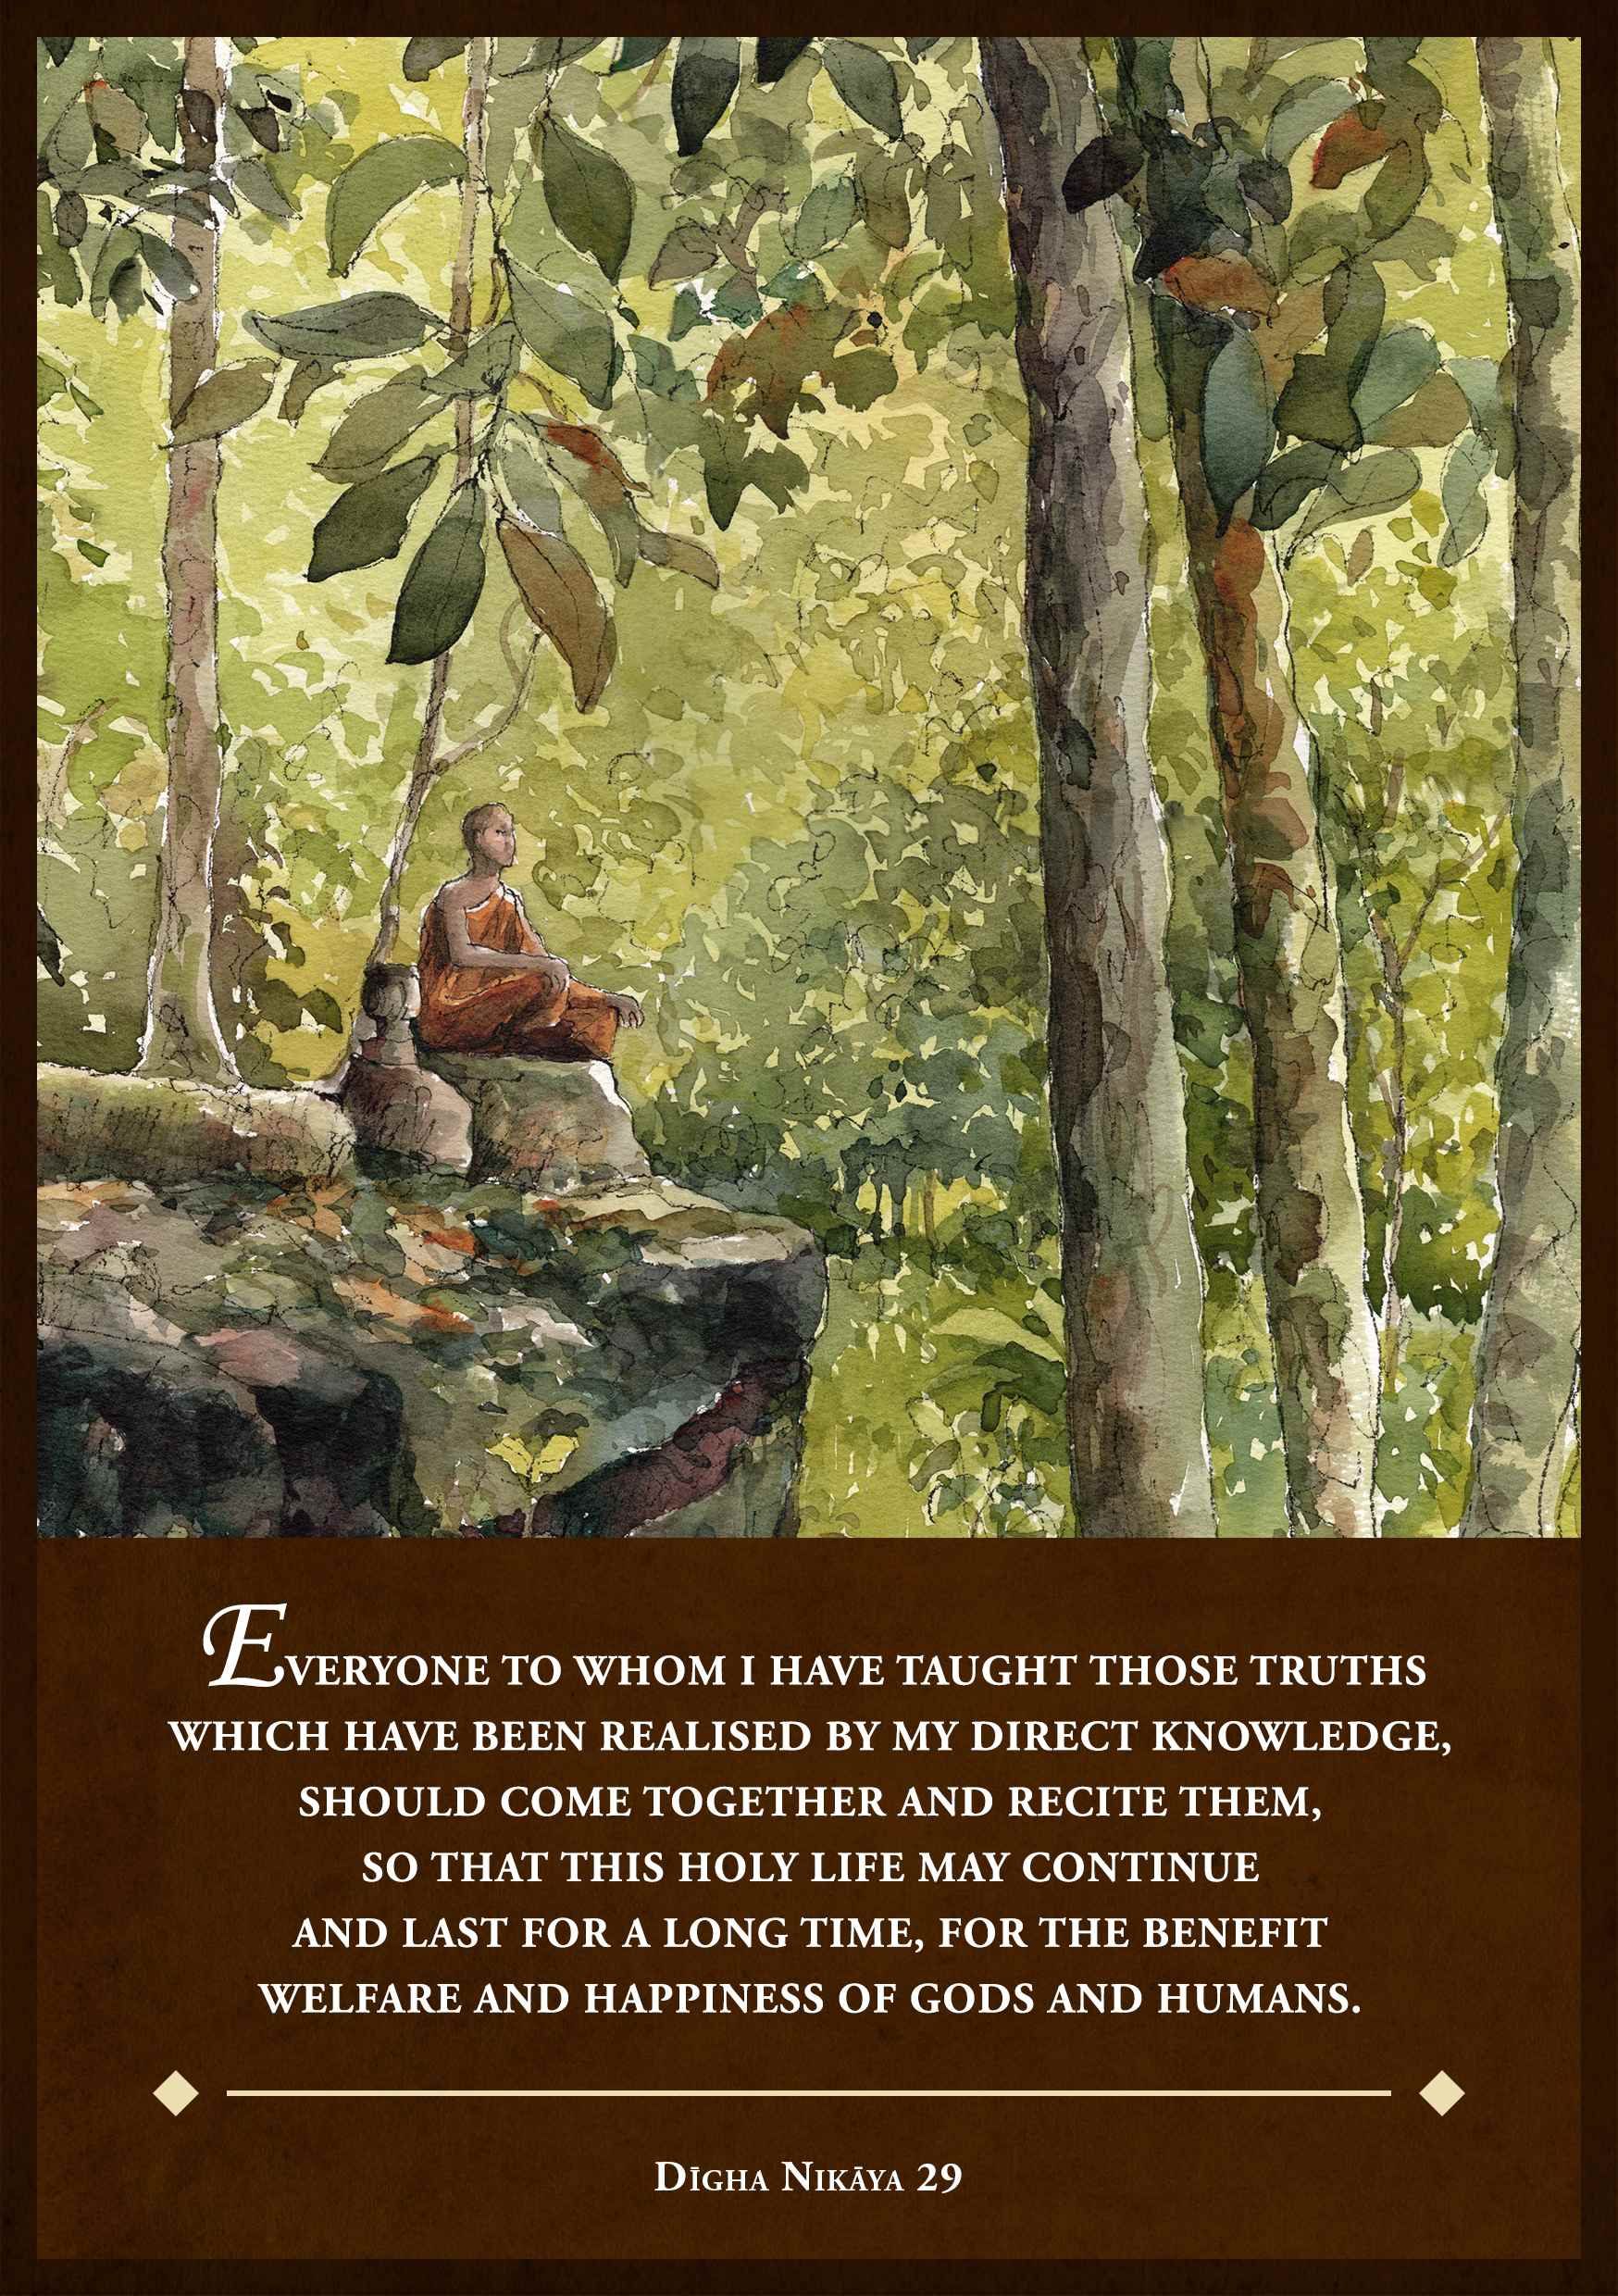
\includegraphics[height=\paperheight]{./back-cover-compressed.jpg}}
\fi

\end{document}
